\documentclass[twoside]{book}

% Packages required by doxygen
\usepackage{calc}
\usepackage{doxygen}
\usepackage{graphicx}
\usepackage[utf8]{inputenc}
\usepackage{makeidx}
\usepackage{multicol}
\usepackage{multirow}
\usepackage{textcomp}
\usepackage[table]{xcolor}

% Font selection
\usepackage[T1]{fontenc}
\usepackage{mathptmx}
\usepackage[scaled=.90]{helvet}
\usepackage{courier}
\usepackage{amssymb}
\usepackage{sectsty}
\renewcommand{\familydefault}{\sfdefault}
\allsectionsfont{%
  \fontseries{bc}\selectfont%
  \color{darkgray}%
}
\renewcommand{\DoxyLabelFont}{%
  \fontseries{bc}\selectfont%
  \color{darkgray}%
}

% Page & text layout
\usepackage{geometry}
\geometry{%
  a4paper,%
  top=2.5cm,%
  bottom=2.5cm,%
  left=2.5cm,%
  right=2.5cm%
}
\tolerance=750
\hfuzz=15pt
\hbadness=750
\setlength{\emergencystretch}{15pt}
\setlength{\parindent}{0cm}
\setlength{\parskip}{0.2cm}
\makeatletter
\renewcommand{\paragraph}{%
  \@startsection{paragraph}{4}{0ex}{-1.0ex}{1.0ex}{%
    \normalfont\normalsize\bfseries\SS@parafont%
  }%
}
\renewcommand{\subparagraph}{%
  \@startsection{subparagraph}{5}{0ex}{-1.0ex}{1.0ex}{%
    \normalfont\normalsize\bfseries\SS@subparafont%
  }%
}
\makeatother

% Headers & footers
\usepackage{fancyhdr}
\pagestyle{fancyplain}
\fancyhead[LE]{\fancyplain{}{\bfseries\thepage}}
\fancyhead[CE]{\fancyplain{}{}}
\fancyhead[RE]{\fancyplain{}{\bfseries\leftmark}}
\fancyhead[LO]{\fancyplain{}{\bfseries\rightmark}}
\fancyhead[CO]{\fancyplain{}{}}
\fancyhead[RO]{\fancyplain{}{\bfseries\thepage}}
\fancyfoot[LE]{\fancyplain{}{}}
\fancyfoot[CE]{\fancyplain{}{}}
\fancyfoot[RE]{\fancyplain{}{\bfseries\scriptsize Generated on Thu Apr 21 2016 21\-:03\-:42 for My Project by Doxygen }}
\fancyfoot[LO]{\fancyplain{}{\bfseries\scriptsize Generated on Thu Apr 21 2016 21\-:03\-:42 for My Project by Doxygen }}
\fancyfoot[CO]{\fancyplain{}{}}
\fancyfoot[RO]{\fancyplain{}{}}
\renewcommand{\footrulewidth}{0.4pt}
\renewcommand{\chaptermark}[1]{%
  \markboth{#1}{}%
}
\renewcommand{\sectionmark}[1]{%
  \markright{\thesection\ #1}%
}

% Indices & bibliography
\usepackage{natbib}
\usepackage[titles]{tocloft}
\setcounter{tocdepth}{3}
\setcounter{secnumdepth}{5}
\makeindex

% Hyperlinks (required, but should be loaded last)
\usepackage{ifpdf}
\ifpdf
  \usepackage[pdftex,pagebackref=true]{hyperref}
\else
  \usepackage[ps2pdf,pagebackref=true]{hyperref}
\fi
\hypersetup{%
  colorlinks=true,%
  linkcolor=blue,%
  citecolor=blue,%
  unicode%
}

% Custom commands
\newcommand{\clearemptydoublepage}{%
  \newpage{\pagestyle{empty}\cleardoublepage}%
}


%===== C O N T E N T S =====

\begin{document}

% Titlepage & ToC
\hypersetup{pageanchor=false}
\pagenumbering{roman}
\begin{titlepage}
\vspace*{7cm}
\begin{center}%
{\Large My Project }\\
\vspace*{1cm}
{\large Generated by Doxygen 1.8.6}\\
\vspace*{0.5cm}
{\small Thu Apr 21 2016 21:03:42}\\
\end{center}
\end{titlepage}
\clearemptydoublepage
\tableofcontents
\clearemptydoublepage
\pagenumbering{arabic}
\hypersetup{pageanchor=true}

%--- Begin generated contents ---
\chapter{Namespace Index}
\section{Namespace List}
Here is a list of all documented namespaces with brief descriptions\-:\begin{DoxyCompactList}
\item\contentsline{section}{\hyperlink{namespaceJava}{Java} }{\pageref{namespaceJava}}{}
\end{DoxyCompactList}

\chapter{Hierarchical Index}
\section{Class Hierarchy}
This inheritance list is sorted roughly, but not completely, alphabetically\+:\begin{DoxyCompactList}
\item \contentsline{section}{com.\+example.\+sel.\+lostfound.\+Category}{\pageref{classcom_1_1example_1_1sel_1_1lostfound_1_1Category}}{}
\item On\+Click\+Listener\begin{DoxyCompactList}
\item \contentsline{section}{com.\+example.\+sel.\+lostfound.\+Main\+Activity}{\pageref{classcom_1_1example_1_1sel_1_1lostfound_1_1MainActivity}}{}
\end{DoxyCompactList}
\item On\+Connection\+Failed\+Listener\begin{DoxyCompactList}
\item \contentsline{section}{com.\+example.\+sel.\+lostfound.\+Main\+Activity}{\pageref{classcom_1_1example_1_1sel_1_1lostfound_1_1MainActivity}}{}
\end{DoxyCompactList}
\item \contentsline{section}{com.\+example.\+sel.\+lostfound.\+Info\+Fragment.\+On\+Fragment\+Interaction\+Listener}{\pageref{interfacecom_1_1example_1_1sel_1_1lostfound_1_1InfoFragment_1_1OnFragmentInteractionListener}}{}
\begin{DoxyCompactList}
\item \contentsline{section}{com.\+example.\+sel.\+lostfound.\+Feed\+Activity}{\pageref{classcom_1_1example_1_1sel_1_1lostfound_1_1FeedActivity}}{}
\end{DoxyCompactList}
\item \contentsline{section}{com.\+example.\+sel.\+lostfound.\+Profile\+Fragment.\+On\+Fragment\+Interaction\+Listener}{\pageref{interfacecom_1_1example_1_1sel_1_1lostfound_1_1ProfileFragment_1_1OnFragmentInteractionListener}}{}
\begin{DoxyCompactList}
\item \contentsline{section}{com.\+example.\+sel.\+lostfound.\+Feed\+Activity}{\pageref{classcom_1_1example_1_1sel_1_1lostfound_1_1FeedActivity}}{}
\end{DoxyCompactList}
\item \contentsline{section}{com.\+example.\+sel.\+lostfound.\+Feed\+Fragment.\+On\+Fragment\+Interaction\+Listener}{\pageref{interfacecom_1_1example_1_1sel_1_1lostfound_1_1FeedFragment_1_1OnFragmentInteractionListener}}{}
\begin{DoxyCompactList}
\item \contentsline{section}{com.\+example.\+sel.\+lostfound.\+Feed\+Activity}{\pageref{classcom_1_1example_1_1sel_1_1lostfound_1_1FeedActivity}}{}
\end{DoxyCompactList}
\item \contentsline{section}{com.\+example.\+sel.\+lostfound.\+Subscribe\+Fragment.\+On\+Fragment\+Interaction\+Listener}{\pageref{interfacecom_1_1example_1_1sel_1_1lostfound_1_1SubscribeFragment_1_1OnFragmentInteractionListener}}{}
\begin{DoxyCompactList}
\item \contentsline{section}{com.\+example.\+sel.\+lostfound.\+Feed\+Activity}{\pageref{classcom_1_1example_1_1sel_1_1lostfound_1_1FeedActivity}}{}
\end{DoxyCompactList}
\item \contentsline{section}{com.\+example.\+sel.\+lostfound.\+Post\+Fragment.\+On\+Fragment\+Interaction\+Listener}{\pageref{interfacecom_1_1example_1_1sel_1_1lostfound_1_1PostFragment_1_1OnFragmentInteractionListener}}{}
\begin{DoxyCompactList}
\item \contentsline{section}{com.\+example.\+sel.\+lostfound.\+Feed\+Activity}{\pageref{classcom_1_1example_1_1sel_1_1lostfound_1_1FeedActivity}}{}
\end{DoxyCompactList}
\item On\+Navigation\+Item\+Selected\+Listener\begin{DoxyCompactList}
\item \contentsline{section}{com.\+example.\+sel.\+lostfound.\+Feed\+Activity}{\pageref{classcom_1_1example_1_1sel_1_1lostfound_1_1FeedActivity}}{}
\end{DoxyCompactList}
\item \contentsline{section}{com.\+example.\+sel.\+lostfound.\+Posts}{\pageref{classcom_1_1example_1_1sel_1_1lostfound_1_1Posts}}{}
\item \contentsline{section}{com.\+example.\+sel.\+lostfound.\+Script\+Runner.\+Script\+Finish\+Listener}{\pageref{interfacecom_1_1example_1_1sel_1_1lostfound_1_1ScriptRunner_1_1ScriptFinishListener}}{}
\item \contentsline{section}{com.\+example.\+sel.\+lostfound.\+User\+Post}{\pageref{classcom_1_1example_1_1sel_1_1lostfound_1_1UserPost}}{}
\item App\+Compat\+Activity\begin{DoxyCompactList}
\item \contentsline{section}{com.\+example.\+sel.\+lostfound.\+Feed\+Activity}{\pageref{classcom_1_1example_1_1sel_1_1lostfound_1_1FeedActivity}}{}
\item \contentsline{section}{com.\+example.\+sel.\+lostfound.\+Main\+Activity}{\pageref{classcom_1_1example_1_1sel_1_1lostfound_1_1MainActivity}}{}
\end{DoxyCompactList}
\item Array\+Adapter\begin{DoxyCompactList}
\item \contentsline{section}{com.\+example.\+sel.\+lostfound.\+Post\+Adapter}{\pageref{classcom_1_1example_1_1sel_1_1lostfound_1_1PostAdapter}}{}
\item \contentsline{section}{com.\+example.\+sel.\+lostfound.\+Spinner\+Adapter}{\pageref{classcom_1_1example_1_1sel_1_1lostfound_1_1SpinnerAdapter}}{}
\item \contentsline{section}{com.\+example.\+sel.\+lostfound.\+Subscribe\+Adapter}{\pageref{classcom_1_1example_1_1sel_1_1lostfound_1_1SubscribeAdapter}}{}
\item \contentsline{section}{com.\+example.\+sel.\+lostfound.\+User\+Post\+Adapter}{\pageref{classcom_1_1example_1_1sel_1_1lostfound_1_1UserPostAdapter}}{}
\end{DoxyCompactList}
\item Async\+Task\begin{DoxyCompactList}
\item \contentsline{section}{com.\+example.\+sel.\+lostfound.\+Backend\+Activity}{\pageref{classcom_1_1example_1_1sel_1_1lostfound_1_1BackendActivity}}{}
\item \contentsline{section}{com.\+example.\+sel.\+lostfound.\+Script\+Runner}{\pageref{classcom_1_1example_1_1sel_1_1lostfound_1_1ScriptRunner}}{}
\end{DoxyCompactList}
\item Fragment\begin{DoxyCompactList}
\item \contentsline{section}{com.\+example.\+sel.\+lostfound.\+Feed\+Fragment}{\pageref{classcom_1_1example_1_1sel_1_1lostfound_1_1FeedFragment}}{}
\item \contentsline{section}{com.\+example.\+sel.\+lostfound.\+Info\+Fragment}{\pageref{classcom_1_1example_1_1sel_1_1lostfound_1_1InfoFragment}}{}
\item \contentsline{section}{com.\+example.\+sel.\+lostfound.\+Post\+Fragment}{\pageref{classcom_1_1example_1_1sel_1_1lostfound_1_1PostFragment}}{}
\item \contentsline{section}{com.\+example.\+sel.\+lostfound.\+Profile\+Fragment}{\pageref{classcom_1_1example_1_1sel_1_1lostfound_1_1ProfileFragment}}{}
\item \contentsline{section}{com.\+example.\+sel.\+lostfound.\+Subscribe\+Fragment}{\pageref{classcom_1_1example_1_1sel_1_1lostfound_1_1SubscribeFragment}}{}
\end{DoxyCompactList}
\end{DoxyCompactList}

\chapter{Class Index}
<<<<<<< HEAD
\section{Class List}
Here are the classes, structs, unions and interfaces with brief descriptions\-:\begin{DoxyCompactList}
\item\contentsline{section}{\hyperlink{classcom_1_1example_1_1sel_1_1lostfound_1_1BackendActivity}{com.\-example.\-sel.\-lostfound.\-Backend\-Activity} \\*Backend Activity class }{\pageref{classcom_1_1example_1_1sel_1_1lostfound_1_1BackendActivity}}{}
\item\contentsline{section}{\hyperlink{classcom_1_1example_1_1sel_1_1lostfound_1_1Category}{com.\-example.\-sel.\-lostfound.\-Category} \\*\hyperlink{classcom_1_1example_1_1sel_1_1lostfound_1_1Category}{Category} class }{\pageref{classcom_1_1example_1_1sel_1_1lostfound_1_1Category}}{}
\item\contentsline{section}{\hyperlink{classcom_1_1example_1_1sel_1_1lostfound_1_1FeedActivity}{com.\-example.\-sel.\-lostfound.\-Feed\-Activity} \\*Feed Activity class }{\pageref{classcom_1_1example_1_1sel_1_1lostfound_1_1FeedActivity}}{}
\item\contentsline{section}{\hyperlink{classcom_1_1example_1_1sel_1_1lostfound_1_1FeedFragment}{com.\-example.\-sel.\-lostfound.\-Feed\-Fragment} }{\pageref{classcom_1_1example_1_1sel_1_1lostfound_1_1FeedFragment}}{}
\item\contentsline{section}{\hyperlink{classcom_1_1example_1_1sel_1_1lostfound_1_1InfoFragment}{com.\-example.\-sel.\-lostfound.\-Info\-Fragment} }{\pageref{classcom_1_1example_1_1sel_1_1lostfound_1_1InfoFragment}}{}
\item\contentsline{section}{\hyperlink{classcom_1_1example_1_1sel_1_1lostfound_1_1MainActivity}{com.\-example.\-sel.\-lostfound.\-Main\-Activity} \\*Main activity class }{\pageref{classcom_1_1example_1_1sel_1_1lostfound_1_1MainActivity}}{}
\item\contentsline{section}{\hyperlink{interfacecom_1_1example_1_1sel_1_1lostfound_1_1InfoFragment_1_1OnFragmentInteractionListener}{com.\-example.\-sel.\-lostfound.\-Info\-Fragment.\-On\-Fragment\-Interaction\-Listener} }{\pageref{interfacecom_1_1example_1_1sel_1_1lostfound_1_1InfoFragment_1_1OnFragmentInteractionListener}}{}
\item\contentsline{section}{\hyperlink{interfacecom_1_1example_1_1sel_1_1lostfound_1_1ProfileFragment_1_1OnFragmentInteractionListener}{com.\-example.\-sel.\-lostfound.\-Profile\-Fragment.\-On\-Fragment\-Interaction\-Listener} }{\pageref{interfacecom_1_1example_1_1sel_1_1lostfound_1_1ProfileFragment_1_1OnFragmentInteractionListener}}{}
\item\contentsline{section}{\hyperlink{interfacecom_1_1example_1_1sel_1_1lostfound_1_1FeedFragment_1_1OnFragmentInteractionListener}{com.\-example.\-sel.\-lostfound.\-Feed\-Fragment.\-On\-Fragment\-Interaction\-Listener} }{\pageref{interfacecom_1_1example_1_1sel_1_1lostfound_1_1FeedFragment_1_1OnFragmentInteractionListener}}{}
\item\contentsline{section}{\hyperlink{interfacecom_1_1example_1_1sel_1_1lostfound_1_1SubscribeFragment_1_1OnFragmentInteractionListener}{com.\-example.\-sel.\-lostfound.\-Subscribe\-Fragment.\-On\-Fragment\-Interaction\-Listener} }{\pageref{interfacecom_1_1example_1_1sel_1_1lostfound_1_1SubscribeFragment_1_1OnFragmentInteractionListener}}{}
\item\contentsline{section}{\hyperlink{interfacecom_1_1example_1_1sel_1_1lostfound_1_1PostFragment_1_1OnFragmentInteractionListener}{com.\-example.\-sel.\-lostfound.\-Post\-Fragment.\-On\-Fragment\-Interaction\-Listener} }{\pageref{interfacecom_1_1example_1_1sel_1_1lostfound_1_1PostFragment_1_1OnFragmentInteractionListener}}{}
=======
\section{\-Class \-List}
\-Here are the classes, structs, unions and interfaces with brief descriptions\-:\begin{DoxyCompactList}
\item\contentsline{section}{\hyperlink{classcom_1_1example_1_1sel_1_1lostfound_1_1BackendActivity}{com.\-example.\-sel.\-lostfound.\-Backend\-Activity} }{\pageref{classcom_1_1example_1_1sel_1_1lostfound_1_1BackendActivity}}{}
\item\contentsline{section}{\hyperlink{classcom_1_1example_1_1sel_1_1lostfound_1_1Category}{com.\-example.\-sel.\-lostfound.\-Category} }{\pageref{classcom_1_1example_1_1sel_1_1lostfound_1_1Category}}{}
\item\contentsline{section}{\hyperlink{classcom_1_1example_1_1sel_1_1lostfound_1_1FeedActivity}{com.\-example.\-sel.\-lostfound.\-Feed\-Activity} }{\pageref{classcom_1_1example_1_1sel_1_1lostfound_1_1FeedActivity}}{}
\item\contentsline{section}{\hyperlink{classcom_1_1example_1_1sel_1_1lostfound_1_1FeedFragment}{com.\-example.\-sel.\-lostfound.\-Feed\-Fragment} }{\pageref{classcom_1_1example_1_1sel_1_1lostfound_1_1FeedFragment}}{}
\item\contentsline{section}{\hyperlink{classcom_1_1example_1_1sel_1_1lostfound_1_1InfoFragment}{com.\-example.\-sel.\-lostfound.\-Info\-Fragment} }{\pageref{classcom_1_1example_1_1sel_1_1lostfound_1_1InfoFragment}}{}
\item\contentsline{section}{\hyperlink{classcom_1_1example_1_1sel_1_1lostfound_1_1MainActivity}{com.\-example.\-sel.\-lostfound.\-Main\-Activity} }{\pageref{classcom_1_1example_1_1sel_1_1lostfound_1_1MainActivity}}{}
\item\contentsline{section}{\hyperlink{interfacecom_1_1example_1_1sel_1_1lostfound_1_1ProfileFragment_1_1OnFragmentInteractionListener}{com.\-example.\-sel.\-lostfound.\-Profile\-Fragment.\-On\-Fragment\-Interaction\-Listener} }{\pageref{interfacecom_1_1example_1_1sel_1_1lostfound_1_1ProfileFragment_1_1OnFragmentInteractionListener}}{}
\item\contentsline{section}{\hyperlink{interfacecom_1_1example_1_1sel_1_1lostfound_1_1InfoFragment_1_1OnFragmentInteractionListener}{com.\-example.\-sel.\-lostfound.\-Info\-Fragment.\-On\-Fragment\-Interaction\-Listener} }{\pageref{interfacecom_1_1example_1_1sel_1_1lostfound_1_1InfoFragment_1_1OnFragmentInteractionListener}}{}
\item\contentsline{section}{\hyperlink{interfacecom_1_1example_1_1sel_1_1lostfound_1_1PostFragment_1_1OnFragmentInteractionListener}{com.\-example.\-sel.\-lostfound.\-Post\-Fragment.\-On\-Fragment\-Interaction\-Listener} }{\pageref{interfacecom_1_1example_1_1sel_1_1lostfound_1_1PostFragment_1_1OnFragmentInteractionListener}}{}
\item\contentsline{section}{\hyperlink{interfacecom_1_1example_1_1sel_1_1lostfound_1_1FeedFragment_1_1OnFragmentInteractionListener}{com.\-example.\-sel.\-lostfound.\-Feed\-Fragment.\-On\-Fragment\-Interaction\-Listener} }{\pageref{interfacecom_1_1example_1_1sel_1_1lostfound_1_1FeedFragment_1_1OnFragmentInteractionListener}}{}
\item\contentsline{section}{\hyperlink{interfacecom_1_1example_1_1sel_1_1lostfound_1_1SubscribeFragment_1_1OnFragmentInteractionListener}{com.\-example.\-sel.\-lostfound.\-Subscribe\-Fragment.\-On\-Fragment\-Interaction\-Listener} }{\pageref{interfacecom_1_1example_1_1sel_1_1lostfound_1_1SubscribeFragment_1_1OnFragmentInteractionListener}}{}
>>>>>>> 0bbb2bc5f31f033d772ef4573f66c50564006509
\item\contentsline{section}{\hyperlink{classcom_1_1example_1_1sel_1_1lostfound_1_1PostAdapter}{com.\-example.\-sel.\-lostfound.\-Post\-Adapter} }{\pageref{classcom_1_1example_1_1sel_1_1lostfound_1_1PostAdapter}}{}
\item\contentsline{section}{\hyperlink{classcom_1_1example_1_1sel_1_1lostfound_1_1PostFragment}{com.\-example.\-sel.\-lostfound.\-Post\-Fragment} }{\pageref{classcom_1_1example_1_1sel_1_1lostfound_1_1PostFragment}}{}
\item\contentsline{section}{\hyperlink{classcom_1_1example_1_1sel_1_1lostfound_1_1Posts}{com.\-example.\-sel.\-lostfound.\-Posts} }{\pageref{classcom_1_1example_1_1sel_1_1lostfound_1_1Posts}}{}
\item\contentsline{section}{\hyperlink{classcom_1_1example_1_1sel_1_1lostfound_1_1ProfileFragment}{com.\-example.\-sel.\-lostfound.\-Profile\-Fragment} }{\pageref{classcom_1_1example_1_1sel_1_1lostfound_1_1ProfileFragment}}{}
\item\contentsline{section}{\hyperlink{interfacecom_1_1example_1_1sel_1_1lostfound_1_1ScriptRunner_1_1ScriptFinishListener}{com.\-example.\-sel.\-lostfound.\-Script\-Runner.\-Script\-Finish\-Listener} }{\pageref{interfacecom_1_1example_1_1sel_1_1lostfound_1_1ScriptRunner_1_1ScriptFinishListener}}{}
\item\contentsline{section}{\hyperlink{classcom_1_1example_1_1sel_1_1lostfound_1_1ScriptRunner}{com.\-example.\-sel.\-lostfound.\-Script\-Runner} }{\pageref{classcom_1_1example_1_1sel_1_1lostfound_1_1ScriptRunner}}{}
\item\contentsline{section}{\hyperlink{classcom_1_1example_1_1sel_1_1lostfound_1_1SpinnerAdapter}{com.\-example.\-sel.\-lostfound.\-Spinner\-Adapter} }{\pageref{classcom_1_1example_1_1sel_1_1lostfound_1_1SpinnerAdapter}}{}
\item\contentsline{section}{\hyperlink{classcom_1_1example_1_1sel_1_1lostfound_1_1SubscribeAdapter}{com.\-example.\-sel.\-lostfound.\-Subscribe\-Adapter} }{\pageref{classcom_1_1example_1_1sel_1_1lostfound_1_1SubscribeAdapter}}{}
\item\contentsline{section}{\hyperlink{classcom_1_1example_1_1sel_1_1lostfound_1_1SubscribeFragment}{com.\-example.\-sel.\-lostfound.\-Subscribe\-Fragment} }{\pageref{classcom_1_1example_1_1sel_1_1lostfound_1_1SubscribeFragment}}{}
\item\contentsline{section}{\hyperlink{classcom_1_1example_1_1sel_1_1lostfound_1_1UserPost}{com.\-example.\-sel.\-lostfound.\-User\-Post} }{\pageref{classcom_1_1example_1_1sel_1_1lostfound_1_1UserPost}}{}
\item\contentsline{section}{\hyperlink{classcom_1_1example_1_1sel_1_1lostfound_1_1UserPostAdapter}{com.\-example.\-sel.\-lostfound.\-User\-Post\-Adapter} }{\pageref{classcom_1_1example_1_1sel_1_1lostfound_1_1UserPostAdapter}}{}
\end{DoxyCompactList}

\chapter{Namespace Documentation}
\hypertarget{namespaceJava}{}\section{Package Java}
\label{namespaceJava}\index{Java@{Java}}


\subsection{Detailed Description}
used 
\chapter{Class Documentation}
\hypertarget{classcom_1_1example_1_1sel_1_1lostfound_1_1BackendActivity}{}\section{com.\+example.\+sel.\+lostfound.\+Backend\+Activity Class Reference}
\label{classcom_1_1example_1_1sel_1_1lostfound_1_1BackendActivity}\index{com.\+example.\+sel.\+lostfound.\+Backend\+Activity@{com.\+example.\+sel.\+lostfound.\+Backend\+Activity}}
Inheritance diagram for com.\+example.\+sel.\+lostfound.\+Backend\+Activity\+:\begin{figure}[H]
\begin{center}
\leavevmode
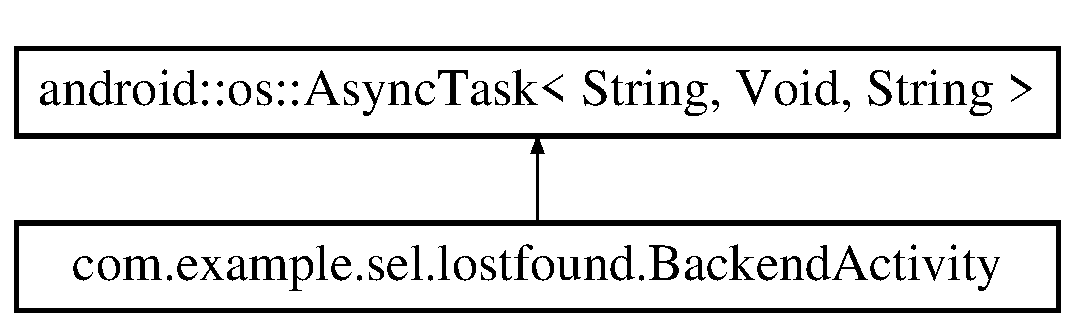
\includegraphics[height=2.000000cm]{classcom_1_1example_1_1sel_1_1lostfound_1_1BackendActivity}
\end{center}
\end{figure}
\subsection*{Protected Member Functions}
\begin{DoxyCompactItemize}
\item 
void {\bfseries on\+Pre\+Execute} ()\hypertarget{classcom_1_1example_1_1sel_1_1lostfound_1_1BackendActivity_a679cd5822b3d0b71b8a947eab9ff6c79}{}\label{classcom_1_1example_1_1sel_1_1lostfound_1_1BackendActivity_a679cd5822b3d0b71b8a947eab9ff6c79}

\item 
String \hyperlink{classcom_1_1example_1_1sel_1_1lostfound_1_1BackendActivity_a4e9c46f342ba6738cdd50c9c75fb3ec7}{do\+In\+Background} (String...\+params)
\begin{DoxyCompactList}\small\item\em function calling php file to check email \end{DoxyCompactList}\item 
void {\bfseries on\+Progress\+Update} (Void...\+values)\hypertarget{classcom_1_1example_1_1sel_1_1lostfound_1_1BackendActivity_a6a2bf0fca03b89c35cd48befe848ee8d}{}\label{classcom_1_1example_1_1sel_1_1lostfound_1_1BackendActivity_a6a2bf0fca03b89c35cd48befe848ee8d}

\item 
void \hyperlink{classcom_1_1example_1_1sel_1_1lostfound_1_1BackendActivity_aa2e67993396f2bf74577e6ff84e16b44}{on\+Post\+Execute} (String result)
\end{DoxyCompactItemize}


\subsection{Member Function Documentation}
\index{com\+::example\+::sel\+::lostfound\+::\+Backend\+Activity@{com\+::example\+::sel\+::lostfound\+::\+Backend\+Activity}!do\+In\+Background@{do\+In\+Background}}
\index{do\+In\+Background@{do\+In\+Background}!com\+::example\+::sel\+::lostfound\+::\+Backend\+Activity@{com\+::example\+::sel\+::lostfound\+::\+Backend\+Activity}}
\subsubsection[{\texorpdfstring{do\+In\+Background(\+String...\+params)}{doInBackground(String...params)}}]{\setlength{\rightskip}{0pt plus 5cm}String com.\+example.\+sel.\+lostfound.\+Backend\+Activity.\+do\+In\+Background (
\begin{DoxyParamCaption}
\item[{String...}]{params}
\end{DoxyParamCaption}
)\hspace{0.3cm}{\ttfamily [inline]}, {\ttfamily [protected]}}\hypertarget{classcom_1_1example_1_1sel_1_1lostfound_1_1BackendActivity_a4e9c46f342ba6738cdd50c9c75fb3ec7}{}\label{classcom_1_1example_1_1sel_1_1lostfound_1_1BackendActivity_a4e9c46f342ba6738cdd50c9c75fb3ec7}


function calling php file to check email 

establishes connection with webserver and validates the email which has been input 
\begin{DoxyParams}{Parameters}
{\em params} & is a string parameter \\
\hline
\end{DoxyParams}
Stores input email to the string variable

url of webserver pointing to check.\+php

adds email to the database

\begin{DoxySeeAlso}{See also}
get\+Query(params) 
\end{DoxySeeAlso}
\index{com\+::example\+::sel\+::lostfound\+::\+Backend\+Activity@{com\+::example\+::sel\+::lostfound\+::\+Backend\+Activity}!on\+Post\+Execute@{on\+Post\+Execute}}
\index{on\+Post\+Execute@{on\+Post\+Execute}!com\+::example\+::sel\+::lostfound\+::\+Backend\+Activity@{com\+::example\+::sel\+::lostfound\+::\+Backend\+Activity}}
\subsubsection[{\texorpdfstring{on\+Post\+Execute(\+String result)}{onPostExecute(String result)}}]{\setlength{\rightskip}{0pt plus 5cm}void com.\+example.\+sel.\+lostfound.\+Backend\+Activity.\+on\+Post\+Execute (
\begin{DoxyParamCaption}
\item[{String}]{result}
\end{DoxyParamCaption}
)\hspace{0.3cm}{\ttfamily [inline]}, {\ttfamily [protected]}}\hypertarget{classcom_1_1example_1_1sel_1_1lostfound_1_1BackendActivity_aa2e67993396f2bf74577e6ff84e16b44}{}\label{classcom_1_1example_1_1sel_1_1lostfound_1_1BackendActivity_aa2e67993396f2bf74577e6ff84e16b44}
Toast display function when email has already been registered 

The documentation for this class was generated from the following file\+:\begin{DoxyCompactItemize}
\item 
Backend\+Activity.\+java\end{DoxyCompactItemize}

\hypertarget{classcom_1_1example_1_1sel_1_1lostfound_1_1Category}{}\section{com.\+example.\+sel.\+lostfound.\+Category Class Reference}
\label{classcom_1_1example_1_1sel_1_1lostfound_1_1Category}\index{com.\+example.\+sel.\+lostfound.\+Category@{com.\+example.\+sel.\+lostfound.\+Category}}


\hyperlink{classcom_1_1example_1_1sel_1_1lostfound_1_1Category}{Category} class.  


\subsection*{Public Member Functions}
\begin{DoxyCompactItemize}
\item 
\hyperlink{classcom_1_1example_1_1sel_1_1lostfound_1_1Category_a01e1a68dd2639ab6bee0007cc1dcf294}{Category} (String category, String cid)
\begin{DoxyCompactList}\small\item\em A constructor with params category and cid. \end{DoxyCompactList}\item 
String \hyperlink{classcom_1_1example_1_1sel_1_1lostfound_1_1Category_a9394ecafd86528fa00554aecbc76ebdb}{get\+Cid} ()\hypertarget{classcom_1_1example_1_1sel_1_1lostfound_1_1Category_a9394ecafd86528fa00554aecbc76ebdb}{}\label{classcom_1_1example_1_1sel_1_1lostfound_1_1Category_a9394ecafd86528fa00554aecbc76ebdb}

\begin{DoxyCompactList}\small\item\em function to get category id \end{DoxyCompactList}\item 
void \hyperlink{classcom_1_1example_1_1sel_1_1lostfound_1_1Category_ae020ac053079f77939440df880c105d7}{set\+Cid} (String cid)\hypertarget{classcom_1_1example_1_1sel_1_1lostfound_1_1Category_ae020ac053079f77939440df880c105d7}{}\label{classcom_1_1example_1_1sel_1_1lostfound_1_1Category_ae020ac053079f77939440df880c105d7}

\begin{DoxyCompactList}\small\item\em function to set category id \end{DoxyCompactList}\item 
String \hyperlink{classcom_1_1example_1_1sel_1_1lostfound_1_1Category_aad1c1ed95ef449791e1e27725ed60314}{get\+Category} ()\hypertarget{classcom_1_1example_1_1sel_1_1lostfound_1_1Category_aad1c1ed95ef449791e1e27725ed60314}{}\label{classcom_1_1example_1_1sel_1_1lostfound_1_1Category_aad1c1ed95ef449791e1e27725ed60314}

\begin{DoxyCompactList}\small\item\em function to get category name \end{DoxyCompactList}\item 
void \hyperlink{classcom_1_1example_1_1sel_1_1lostfound_1_1Category_a64b466d2eed1b6eafe4d2a5785aaf7e4}{set\+Category} (String category)\hypertarget{classcom_1_1example_1_1sel_1_1lostfound_1_1Category_a64b466d2eed1b6eafe4d2a5785aaf7e4}{}\label{classcom_1_1example_1_1sel_1_1lostfound_1_1Category_a64b466d2eed1b6eafe4d2a5785aaf7e4}

\begin{DoxyCompactList}\small\item\em function to set category name \end{DoxyCompactList}\end{DoxyCompactItemize}


\subsection{Detailed Description}
\hyperlink{classcom_1_1example_1_1sel_1_1lostfound_1_1Category}{Category} class. 

Created by achu on 12-\/04-\/2016.

class implementing categories 

\subsection{Constructor \& Destructor Documentation}
\index{com\+::example\+::sel\+::lostfound\+::\+Category@{com\+::example\+::sel\+::lostfound\+::\+Category}!Category@{Category}}
\index{Category@{Category}!com\+::example\+::sel\+::lostfound\+::\+Category@{com\+::example\+::sel\+::lostfound\+::\+Category}}
\subsubsection[{\texorpdfstring{Category(\+String category, String cid)}{Category(String category, String cid)}}]{\setlength{\rightskip}{0pt plus 5cm}com.\+example.\+sel.\+lostfound.\+Category.\+Category (
\begin{DoxyParamCaption}
\item[{String}]{category, }
\item[{String}]{cid}
\end{DoxyParamCaption}
)\hspace{0.3cm}{\ttfamily [inline]}}\hypertarget{classcom_1_1example_1_1sel_1_1lostfound_1_1Category_a01e1a68dd2639ab6bee0007cc1dcf294}{}\label{classcom_1_1example_1_1sel_1_1lostfound_1_1Category_a01e1a68dd2639ab6bee0007cc1dcf294}


A constructor with params category and cid. 

\hyperlink{classcom_1_1example_1_1sel_1_1lostfound_1_1Category}{Category} id 

The documentation for this class was generated from the following file\+:\begin{DoxyCompactItemize}
\item 
Category.\+java\end{DoxyCompactItemize}

<<<<<<< HEAD
\hypertarget{classcom_1_1example_1_1sel_1_1lostfound_1_1FeedActivity}{\section{com.\-example.\-sel.\-lostfound.\-Feed\-Activity Class Reference}
\label{classcom_1_1example_1_1sel_1_1lostfound_1_1FeedActivity}\index{com.\-example.\-sel.\-lostfound.\-Feed\-Activity@{com.\-example.\-sel.\-lostfound.\-Feed\-Activity}}
}


Feed Activity class.  


Inheritance diagram for com.\-example.\-sel.\-lostfound.\-Feed\-Activity\-:\begin{figure}[H]
\begin{center}
\leavevmode
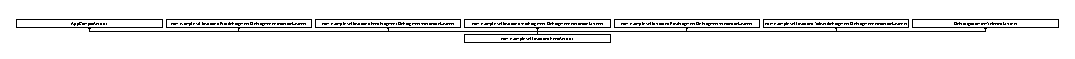
\includegraphics[height=0.347826cm]{classcom_1_1example_1_1sel_1_1lostfound_1_1FeedActivity}
\end{center}
\end{figure}
\subsection*{Public Member Functions}
\begin{DoxyCompactItemize}
\item 
void \hyperlink{classcom_1_1example_1_1sel_1_1lostfound_1_1FeedActivity_a92ef1347dacbec013be0cc6eaf19e680}{on\-Back\-Pressed} ()
\item 
boolean \hyperlink{classcom_1_1example_1_1sel_1_1lostfound_1_1FeedActivity_a11b2b6ec46e07d2248259b101dd4f699}{on\-Create\-Options\-Menu} (Menu menu)
\item 
\hypertarget{classcom_1_1example_1_1sel_1_1lostfound_1_1FeedActivity_a30ac1d8cd6a1f8f4a17546f894ee0150}{boolean {\bfseries on\-Options\-Item\-Selected} (Menu\-Item item)}\label{classcom_1_1example_1_1sel_1_1lostfound_1_1FeedActivity_a30ac1d8cd6a1f8f4a17546f894ee0150}

\item 
boolean \hyperlink{classcom_1_1example_1_1sel_1_1lostfound_1_1FeedActivity_ac1e5f59e54f8b0adfcfcd7999c7d5d3d}{on\-Navigation\-Item\-Selected} (Menu\-Item item)
\item 
\hypertarget{classcom_1_1example_1_1sel_1_1lostfound_1_1FeedActivity_a7dab67bae2a8451acea819995f6e10b8}{void {\bfseries on\-Profile\-Fragment\-Interaction} (String string)}\label{classcom_1_1example_1_1sel_1_1lostfound_1_1FeedActivity_a7dab67bae2a8451acea819995f6e10b8}

\item 
\hypertarget{classcom_1_1example_1_1sel_1_1lostfound_1_1FeedActivity_a4d16fc6e0aa78d30aa10142e5e2584ac}{void {\bfseries on\-Info\-Fragment\-Interaction} (String string)}\label{classcom_1_1example_1_1sel_1_1lostfound_1_1FeedActivity_a4d16fc6e0aa78d30aa10142e5e2584ac}

\item 
\hypertarget{classcom_1_1example_1_1sel_1_1lostfound_1_1FeedActivity_a93cd51363a21d0dd0368eca17f91aa31}{void {\bfseries on\-Post\-Fragment\-Interaction} (String string)}\label{classcom_1_1example_1_1sel_1_1lostfound_1_1FeedActivity_a93cd51363a21d0dd0368eca17f91aa31}

\item 
\hypertarget{classcom_1_1example_1_1sel_1_1lostfound_1_1FeedActivity_a387420f45593f43ed8a998fabd4e1840}{void {\bfseries on\-Feed\-Fragment\-Interaction} (String string)}\label{classcom_1_1example_1_1sel_1_1lostfound_1_1FeedActivity_a387420f45593f43ed8a998fabd4e1840}

\item 
\hypertarget{classcom_1_1example_1_1sel_1_1lostfound_1_1FeedActivity_a2933085fa5342bd11b601c37120d850e}{void {\bfseries on\-Subscribe\-Fragment\-Interaction} (String string)}\label{classcom_1_1example_1_1sel_1_1lostfound_1_1FeedActivity_a2933085fa5342bd11b601c37120d850e}

\item 
\hypertarget{classcom_1_1example_1_1sel_1_1lostfound_1_1FeedActivity_a15280442a0b2314b06299d1d57318827}{void {\bfseries on\-Fragment\-Interaction} (Uri uri)}\label{classcom_1_1example_1_1sel_1_1lostfound_1_1FeedActivity_a15280442a0b2314b06299d1d57318827}

\end{DoxyCompactItemize}
\subsection*{Protected Member Functions}
\begin{DoxyCompactItemize}
\item 
void \hyperlink{classcom_1_1example_1_1sel_1_1lostfound_1_1FeedActivity_a27dee5594c91dcb9216364c9556c4af7}{on\-Create} (Bundle saved\-Instance\-State)
\end{DoxyCompactItemize}
\subsection*{Static Protected Attributes}
\begin{DoxyCompactItemize}
\item 
static String \hyperlink{classcom_1_1example_1_1sel_1_1lostfound_1_1FeedActivity_a485e807a263274d664ce60fae23ebb45}{ptype} = \char`\"{}\char`\"{}
\end{DoxyCompactItemize}


\subsection{Detailed Description}
Feed Activity class. 

Created by Rohit G on 3/31/2016. implementing navigation bar. 

\subsection{Member Function Documentation}
\hypertarget{classcom_1_1example_1_1sel_1_1lostfound_1_1FeedActivity_a92ef1347dacbec013be0cc6eaf19e680}{\index{com\-::example\-::sel\-::lostfound\-::\-Feed\-Activity@{com\-::example\-::sel\-::lostfound\-::\-Feed\-Activity}!on\-Back\-Pressed@{on\-Back\-Pressed}}
\index{on\-Back\-Pressed@{on\-Back\-Pressed}!com::example::sel::lostfound::FeedActivity@{com\-::example\-::sel\-::lostfound\-::\-Feed\-Activity}}
\subsubsection[{on\-Back\-Pressed}]{\setlength{\rightskip}{0pt plus 5cm}void com.\-example.\-sel.\-lostfound.\-Feed\-Activity.\-on\-Back\-Pressed (
\begin{DoxyParamCaption}
{}
\end{DoxyParamCaption}
)\hspace{0.3cm}{\ttfamily [inline]}}}\label{classcom_1_1example_1_1sel_1_1lostfound_1_1FeedActivity_a92ef1347dacbec013be0cc6eaf19e680}
function implementing actions when 'back' is pressed while navigation bar is open \hypertarget{classcom_1_1example_1_1sel_1_1lostfound_1_1FeedActivity_a27dee5594c91dcb9216364c9556c4af7}{\index{com\-::example\-::sel\-::lostfound\-::\-Feed\-Activity@{com\-::example\-::sel\-::lostfound\-::\-Feed\-Activity}!on\-Create@{on\-Create}}
\index{on\-Create@{on\-Create}!com::example::sel::lostfound::FeedActivity@{com\-::example\-::sel\-::lostfound\-::\-Feed\-Activity}}
\subsubsection[{on\-Create}]{\setlength{\rightskip}{0pt plus 5cm}void com.\-example.\-sel.\-lostfound.\-Feed\-Activity.\-on\-Create (
\begin{DoxyParamCaption}
\item[{Bundle}]{saved\-Instance\-State}
\end{DoxyParamCaption}
)\hspace{0.3cm}{\ttfamily [inline]}, {\ttfamily [protected]}}}\label{classcom_1_1example_1_1sel_1_1lostfound_1_1FeedActivity_a27dee5594c91dcb9216364c9556c4af7}
function defining actions done when the activity is started or created. home screen content (showing profile initially)

display signed in message along with user's email id

opening navigation bar

$<$ display user's name on navigation bar

$<$ display user's email id on navigation bar

to display picture \hypertarget{classcom_1_1example_1_1sel_1_1lostfound_1_1FeedActivity_a11b2b6ec46e07d2248259b101dd4f699}{\index{com\-::example\-::sel\-::lostfound\-::\-Feed\-Activity@{com\-::example\-::sel\-::lostfound\-::\-Feed\-Activity}!on\-Create\-Options\-Menu@{on\-Create\-Options\-Menu}}
\index{on\-Create\-Options\-Menu@{on\-Create\-Options\-Menu}!com::example::sel::lostfound::FeedActivity@{com\-::example\-::sel\-::lostfound\-::\-Feed\-Activity}}
\subsubsection[{on\-Create\-Options\-Menu}]{\setlength{\rightskip}{0pt plus 5cm}boolean com.\-example.\-sel.\-lostfound.\-Feed\-Activity.\-on\-Create\-Options\-Menu (
\begin{DoxyParamCaption}
\item[{Menu}]{menu}
\end{DoxyParamCaption}
)\hspace{0.3cm}{\ttfamily [inline]}}}\label{classcom_1_1example_1_1sel_1_1lostfound_1_1FeedActivity_a11b2b6ec46e07d2248259b101dd4f699}
shows the options in the menu as result of opening the navigation bar \hypertarget{classcom_1_1example_1_1sel_1_1lostfound_1_1FeedActivity_ac1e5f59e54f8b0adfcfcd7999c7d5d3d}{\index{com\-::example\-::sel\-::lostfound\-::\-Feed\-Activity@{com\-::example\-::sel\-::lostfound\-::\-Feed\-Activity}!on\-Navigation\-Item\-Selected@{on\-Navigation\-Item\-Selected}}
\index{on\-Navigation\-Item\-Selected@{on\-Navigation\-Item\-Selected}!com::example::sel::lostfound::FeedActivity@{com\-::example\-::sel\-::lostfound\-::\-Feed\-Activity}}
\subsubsection[{on\-Navigation\-Item\-Selected}]{\setlength{\rightskip}{0pt plus 5cm}boolean com.\-example.\-sel.\-lostfound.\-Feed\-Activity.\-on\-Navigation\-Item\-Selected (
\begin{DoxyParamCaption}
\item[{Menu\-Item}]{item}
\end{DoxyParamCaption}
)\hspace{0.3cm}{\ttfamily [inline]}}}\label{classcom_1_1example_1_1sel_1_1lostfound_1_1FeedActivity_ac1e5f59e54f8b0adfcfcd7999c7d5d3d}
function implementing actions on selecting a particular row in navigation bar. $<$ variable id stores item id selected by user

profile page opened as result of selection of 'profile' on navigation bar

feed page opened as result of selection of 'feeds' on navigation bar

post page opened as result of selection of 'post' on navigation bar

subscribe page opened as result of selection of 'subscriptions' on navigation bar

info page opened as result of selection of Info on navigation bar

sign out activity implemented

closes the navigation bar 

\subsection{Member Data Documentation}
\hypertarget{classcom_1_1example_1_1sel_1_1lostfound_1_1FeedActivity_a485e807a263274d664ce60fae23ebb45}{\index{com\-::example\-::sel\-::lostfound\-::\-Feed\-Activity@{com\-::example\-::sel\-::lostfound\-::\-Feed\-Activity}!ptype@{ptype}}
\index{ptype@{ptype}!com::example::sel::lostfound::FeedActivity@{com\-::example\-::sel\-::lostfound\-::\-Feed\-Activity}}
\subsubsection[{ptype}]{\setlength{\rightskip}{0pt plus 5cm}String com.\-example.\-sel.\-lostfound.\-Feed\-Activity.\-ptype = \char`\"{}\char`\"{}\hspace{0.3cm}{\ttfamily [static]}, {\ttfamily [protected]}}}\label{classcom_1_1example_1_1sel_1_1lostfound_1_1FeedActivity_a485e807a263274d664ce60fae23ebb45}
variable of type string 

The documentation for this class was generated from the following file\-:\begin{DoxyCompactItemize}
\item 
Feed\-Activity.\-java\end{DoxyCompactItemize}
=======
\hypertarget{classcom_1_1example_1_1sel_1_1lostfound_1_1FeedActivity}{\section{com.\-example.\-sel.\-lostfound.\-Feed\-Activity \-Class \-Reference}
\label{classcom_1_1example_1_1sel_1_1lostfound_1_1FeedActivity}\index{com.\-example.\-sel.\-lostfound.\-Feed\-Activity@{com.\-example.\-sel.\-lostfound.\-Feed\-Activity}}
}
\-Inheritance diagram for com.\-example.\-sel.\-lostfound.\-Feed\-Activity\-:\begin{figure}[H]
\begin{center}
\leavevmode
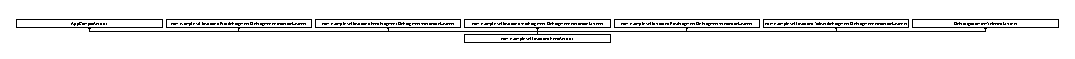
\includegraphics[height=0.486957cm]{classcom_1_1example_1_1sel_1_1lostfound_1_1FeedActivity}
\end{center}
\end{figure}
\subsection*{\-Classes}
\begin{DoxyCompactItemize}
\item 
class {\bfseries \-Download\-Image\-Task}
\end{DoxyCompactItemize}
\subsection*{\-Public \-Member \-Functions}
\begin{DoxyCompactItemize}
\item 
\hypertarget{classcom_1_1example_1_1sel_1_1lostfound_1_1FeedActivity_a92ef1347dacbec013be0cc6eaf19e680}{void {\bfseries on\-Back\-Pressed} ()}\label{classcom_1_1example_1_1sel_1_1lostfound_1_1FeedActivity_a92ef1347dacbec013be0cc6eaf19e680}

\item 
\hypertarget{classcom_1_1example_1_1sel_1_1lostfound_1_1FeedActivity_a11b2b6ec46e07d2248259b101dd4f699}{boolean {\bfseries on\-Create\-Options\-Menu} (\-Menu menu)}\label{classcom_1_1example_1_1sel_1_1lostfound_1_1FeedActivity_a11b2b6ec46e07d2248259b101dd4f699}

\item 
\hypertarget{classcom_1_1example_1_1sel_1_1lostfound_1_1FeedActivity_a30ac1d8cd6a1f8f4a17546f894ee0150}{boolean {\bfseries on\-Options\-Item\-Selected} (\-Menu\-Item item)}\label{classcom_1_1example_1_1sel_1_1lostfound_1_1FeedActivity_a30ac1d8cd6a1f8f4a17546f894ee0150}

\item 
\hypertarget{classcom_1_1example_1_1sel_1_1lostfound_1_1FeedActivity_ac1e5f59e54f8b0adfcfcd7999c7d5d3d}{boolean {\bfseries on\-Navigation\-Item\-Selected} (\-Menu\-Item item)}\label{classcom_1_1example_1_1sel_1_1lostfound_1_1FeedActivity_ac1e5f59e54f8b0adfcfcd7999c7d5d3d}

\item 
\hypertarget{classcom_1_1example_1_1sel_1_1lostfound_1_1FeedActivity_a7dab67bae2a8451acea819995f6e10b8}{void {\bfseries on\-Profile\-Fragment\-Interaction} (\-String string)}\label{classcom_1_1example_1_1sel_1_1lostfound_1_1FeedActivity_a7dab67bae2a8451acea819995f6e10b8}

\item 
\hypertarget{classcom_1_1example_1_1sel_1_1lostfound_1_1FeedActivity_a4d16fc6e0aa78d30aa10142e5e2584ac}{void {\bfseries on\-Info\-Fragment\-Interaction} (\-String string)}\label{classcom_1_1example_1_1sel_1_1lostfound_1_1FeedActivity_a4d16fc6e0aa78d30aa10142e5e2584ac}

\item 
\hypertarget{classcom_1_1example_1_1sel_1_1lostfound_1_1FeedActivity_a93cd51363a21d0dd0368eca17f91aa31}{void {\bfseries on\-Post\-Fragment\-Interaction} (\-String string)}\label{classcom_1_1example_1_1sel_1_1lostfound_1_1FeedActivity_a93cd51363a21d0dd0368eca17f91aa31}

\item 
\hypertarget{classcom_1_1example_1_1sel_1_1lostfound_1_1FeedActivity_a387420f45593f43ed8a998fabd4e1840}{void {\bfseries on\-Feed\-Fragment\-Interaction} (\-String string)}\label{classcom_1_1example_1_1sel_1_1lostfound_1_1FeedActivity_a387420f45593f43ed8a998fabd4e1840}

\item 
\hypertarget{classcom_1_1example_1_1sel_1_1lostfound_1_1FeedActivity_a2933085fa5342bd11b601c37120d850e}{void {\bfseries on\-Subscribe\-Fragment\-Interaction} (\-String string)}\label{classcom_1_1example_1_1sel_1_1lostfound_1_1FeedActivity_a2933085fa5342bd11b601c37120d850e}

\item 
\hypertarget{classcom_1_1example_1_1sel_1_1lostfound_1_1FeedActivity_a15280442a0b2314b06299d1d57318827}{void {\bfseries on\-Fragment\-Interaction} (\-Uri uri)}\label{classcom_1_1example_1_1sel_1_1lostfound_1_1FeedActivity_a15280442a0b2314b06299d1d57318827}

\end{DoxyCompactItemize}
\subsection*{\-Protected \-Member \-Functions}
\begin{DoxyCompactItemize}
\item 
\hypertarget{classcom_1_1example_1_1sel_1_1lostfound_1_1FeedActivity_a27dee5594c91dcb9216364c9556c4af7}{void {\bfseries on\-Create} (\-Bundle saved\-Instance\-State)}\label{classcom_1_1example_1_1sel_1_1lostfound_1_1FeedActivity_a27dee5594c91dcb9216364c9556c4af7}

\end{DoxyCompactItemize}
\subsection*{\-Static \-Protected \-Attributes}
\begin{DoxyCompactItemize}
\item 
\hypertarget{classcom_1_1example_1_1sel_1_1lostfound_1_1FeedActivity_a485e807a263274d664ce60fae23ebb45}{static \-String {\bfseries ptype} = \char`\"{}\char`\"{}}\label{classcom_1_1example_1_1sel_1_1lostfound_1_1FeedActivity_a485e807a263274d664ce60fae23ebb45}

\end{DoxyCompactItemize}
\subsection*{\-Package \-Attributes}
\begin{DoxyCompactItemize}
\item 
\hypertarget{classcom_1_1example_1_1sel_1_1lostfound_1_1FeedActivity_a51b8f541b1fa87bae79552e02354112c}{\-Navigation\-View {\bfseries navigation\-View} = null}\label{classcom_1_1example_1_1sel_1_1lostfound_1_1FeedActivity_a51b8f541b1fa87bae79552e02354112c}

\item 
\hypertarget{classcom_1_1example_1_1sel_1_1lostfound_1_1FeedActivity_a8513e4158e73b84a7fd07415fded1478}{\-Toolbar {\bfseries toolbar} = null}\label{classcom_1_1example_1_1sel_1_1lostfound_1_1FeedActivity_a8513e4158e73b84a7fd07415fded1478}

\item 
\hypertarget{classcom_1_1example_1_1sel_1_1lostfound_1_1FeedActivity_ad25f59821cace19c4a041b416d524e6b}{\-Text\-View {\bfseries name\-Text}}\label{classcom_1_1example_1_1sel_1_1lostfound_1_1FeedActivity_ad25f59821cace19c4a041b416d524e6b}

\item 
\hypertarget{classcom_1_1example_1_1sel_1_1lostfound_1_1FeedActivity_aba980cd82976141d8376704b9b3a4561}{\-Text\-View {\bfseries email\-Text}}\label{classcom_1_1example_1_1sel_1_1lostfound_1_1FeedActivity_aba980cd82976141d8376704b9b3a4561}

\end{DoxyCompactItemize}


\subsection{\-Detailed \-Description}
\-Created by \-Rohit \-G on 3/31/2016. 

\-The documentation for this class was generated from the following file\-:\begin{DoxyCompactItemize}
\item 
\-Feed\-Activity.\-java\end{DoxyCompactItemize}
>>>>>>> 0bbb2bc5f31f033d772ef4573f66c50564006509

\hypertarget{classcom_1_1example_1_1sel_1_1lostfound_1_1FeedFragment}{}\section{com.\+example.\+sel.\+lostfound.\+Feed\+Fragment Class Reference}
\label{classcom_1_1example_1_1sel_1_1lostfound_1_1FeedFragment}\index{com.\+example.\+sel.\+lostfound.\+Feed\+Fragment@{com.\+example.\+sel.\+lostfound.\+Feed\+Fragment}}


A class implementing fragment of feed when its clicked on navigation bar.  


Inheritance diagram for com.\+example.\+sel.\+lostfound.\+Feed\+Fragment\+:\begin{figure}[H]
\begin{center}
\leavevmode
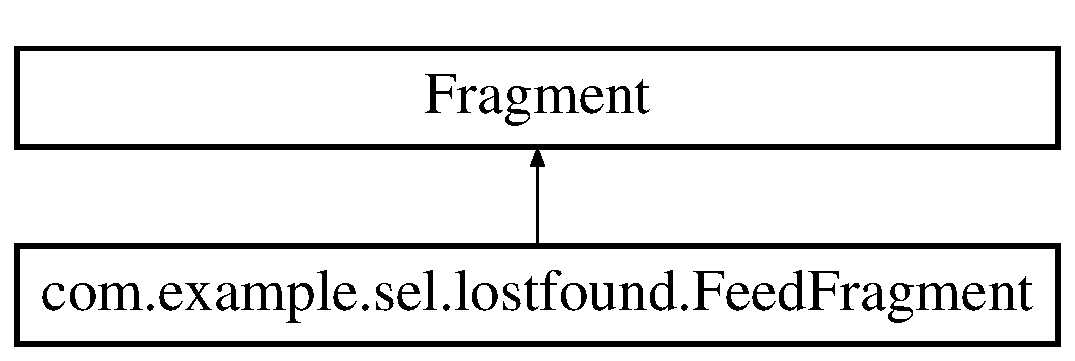
\includegraphics[height=2.000000cm]{classcom_1_1example_1_1sel_1_1lostfound_1_1FeedFragment}
\end{center}
\end{figure}
\subsection*{Classes}
\begin{DoxyCompactItemize}
\item 
interface \hyperlink{interfacecom_1_1example_1_1sel_1_1lostfound_1_1FeedFragment_1_1OnFragmentInteractionListener}{On\+Fragment\+Interaction\+Listener}
\end{DoxyCompactItemize}
\subsection*{Public Member Functions}
\begin{DoxyCompactItemize}
\item 
void \hyperlink{classcom_1_1example_1_1sel_1_1lostfound_1_1FeedFragment_a027942ee12844b17c604195b91f9948d}{on\+Create} (Bundle saved\+Instance\+State)\hypertarget{classcom_1_1example_1_1sel_1_1lostfound_1_1FeedFragment_a027942ee12844b17c604195b91f9948d}{}\label{classcom_1_1example_1_1sel_1_1lostfound_1_1FeedFragment_a027942ee12844b17c604195b91f9948d}

\begin{DoxyCompactList}\small\item\em function on clicking \textquotesingle{}Feed\textquotesingle{} on the navigation bar \end{DoxyCompactList}\item 
void \hyperlink{classcom_1_1example_1_1sel_1_1lostfound_1_1FeedFragment_abb8194bc01339ece4f650c3b7e716a5f}{on\+Activity\+Created} (Bundle saved\+Instance\+State)
\begin{DoxyCompactList}\small\item\em function on opening feed page \end{DoxyCompactList}\item 
View {\bfseries on\+Create\+View} (Layout\+Inflater inflater, View\+Group container, Bundle saved\+Instance\+State)\hypertarget{classcom_1_1example_1_1sel_1_1lostfound_1_1FeedFragment_a4e2cc79785d7392af2839c0b3900b12b}{}\label{classcom_1_1example_1_1sel_1_1lostfound_1_1FeedFragment_a4e2cc79785d7392af2839c0b3900b12b}

\item 
void {\bfseries on\+Button\+Pressed} (Uri uri)\hypertarget{classcom_1_1example_1_1sel_1_1lostfound_1_1FeedFragment_a4a39372816f2c53d6ff1b3d12be98c23}{}\label{classcom_1_1example_1_1sel_1_1lostfound_1_1FeedFragment_a4a39372816f2c53d6ff1b3d12be98c23}

\item 
void {\bfseries on\+Attach} (Context context)\hypertarget{classcom_1_1example_1_1sel_1_1lostfound_1_1FeedFragment_a63947b4cbebd081d42113ff157a2f6b0}{}\label{classcom_1_1example_1_1sel_1_1lostfound_1_1FeedFragment_a63947b4cbebd081d42113ff157a2f6b0}

\item 
void {\bfseries on\+Detach} ()\hypertarget{classcom_1_1example_1_1sel_1_1lostfound_1_1FeedFragment_a1cc06e44e371cfc7f6b0bb5da15f78f0}{}\label{classcom_1_1example_1_1sel_1_1lostfound_1_1FeedFragment_a1cc06e44e371cfc7f6b0bb5da15f78f0}

\end{DoxyCompactItemize}
\subsection*{Static Public Member Functions}
\begin{DoxyCompactItemize}
\item 
static \hyperlink{classcom_1_1example_1_1sel_1_1lostfound_1_1FeedFragment}{Feed\+Fragment} \hyperlink{classcom_1_1example_1_1sel_1_1lostfound_1_1FeedFragment_a63f279103cc59000c74087d6addb351f}{new\+Instance} (String param1, String param2)
\begin{DoxyCompactList}\small\item\em new instance of fragment \end{DoxyCompactList}\end{DoxyCompactItemize}


\subsection{Detailed Description}
A class implementing fragment of feed when its clicked on navigation bar. 

A simple \hyperlink{}{Fragment} subclass. Activities that contain this fragment must implement the \hyperlink{interfacecom_1_1example_1_1sel_1_1lostfound_1_1FeedFragment_1_1OnFragmentInteractionListener}{Feed\+Fragment.\+On\+Fragment\+Interaction\+Listener} interface to handle interaction events. Use the \hyperlink{classcom_1_1example_1_1sel_1_1lostfound_1_1FeedFragment_a63f279103cc59000c74087d6addb351f}{Feed\+Fragment\#new\+Instance} factory method to create an instance of this fragment. 

\subsection{Member Function Documentation}
\index{com\+::example\+::sel\+::lostfound\+::\+Feed\+Fragment@{com\+::example\+::sel\+::lostfound\+::\+Feed\+Fragment}!new\+Instance@{new\+Instance}}
\index{new\+Instance@{new\+Instance}!com\+::example\+::sel\+::lostfound\+::\+Feed\+Fragment@{com\+::example\+::sel\+::lostfound\+::\+Feed\+Fragment}}
\subsubsection[{\texorpdfstring{new\+Instance(\+String param1, String param2)}{newInstance(String param1, String param2)}}]{\setlength{\rightskip}{0pt plus 5cm}static {\bf Feed\+Fragment} com.\+example.\+sel.\+lostfound.\+Feed\+Fragment.\+new\+Instance (
\begin{DoxyParamCaption}
\item[{String}]{param1, }
\item[{String}]{param2}
\end{DoxyParamCaption}
)\hspace{0.3cm}{\ttfamily [inline]}, {\ttfamily [static]}}\hypertarget{classcom_1_1example_1_1sel_1_1lostfound_1_1FeedFragment_a63f279103cc59000c74087d6addb351f}{}\label{classcom_1_1example_1_1sel_1_1lostfound_1_1FeedFragment_a63f279103cc59000c74087d6addb351f}


new instance of fragment 

Use this factory method to create a new instance of this fragment using the provided parameters.


\begin{DoxyParams}{Parameters}
{\em param1} & Parameter 1. \\
\hline
{\em param2} & Parameter 2. \\
\hline
\end{DoxyParams}
\begin{DoxyReturn}{Returns}
A new instance of fragment \hyperlink{classcom_1_1example_1_1sel_1_1lostfound_1_1FeedFragment}{Feed\+Fragment}. 
\end{DoxyReturn}
\index{com\+::example\+::sel\+::lostfound\+::\+Feed\+Fragment@{com\+::example\+::sel\+::lostfound\+::\+Feed\+Fragment}!on\+Activity\+Created@{on\+Activity\+Created}}
\index{on\+Activity\+Created@{on\+Activity\+Created}!com\+::example\+::sel\+::lostfound\+::\+Feed\+Fragment@{com\+::example\+::sel\+::lostfound\+::\+Feed\+Fragment}}
\subsubsection[{\texorpdfstring{on\+Activity\+Created(\+Bundle saved\+Instance\+State)}{onActivityCreated(Bundle savedInstanceState)}}]{\setlength{\rightskip}{0pt plus 5cm}void com.\+example.\+sel.\+lostfound.\+Feed\+Fragment.\+on\+Activity\+Created (
\begin{DoxyParamCaption}
\item[{Bundle}]{saved\+Instance\+State}
\end{DoxyParamCaption}
)\hspace{0.3cm}{\ttfamily [inline]}}\hypertarget{classcom_1_1example_1_1sel_1_1lostfound_1_1FeedFragment_abb8194bc01339ece4f650c3b7e716a5f}{}\label{classcom_1_1example_1_1sel_1_1lostfound_1_1FeedFragment_abb8194bc01339ece4f650c3b7e716a5f}


function on opening feed page 

$<$list view instance

$<$ spinner for dropdown list of found or lost type

dropdown lost

dropdown found

function on selecting type in dropdown list

function on selecting type of feed you want to browse(found/lost)

Here you get the current item (a User object) that is selected by its position

display type

extracting information from database table \textquotesingle{}post\textquotesingle{}

adding a new post in the \textquotesingle{}feed\textquotesingle{} page 

The documentation for this class was generated from the following file\+:\begin{DoxyCompactItemize}
\item 
Feed\+Fragment.\+java\end{DoxyCompactItemize}

\hypertarget{classcom_1_1example_1_1sel_1_1lostfound_1_1InfoFragment}{\section{com.\-example.\-sel.\-lostfound.\-Info\-Fragment Class Reference}
\label{classcom_1_1example_1_1sel_1_1lostfound_1_1InfoFragment}\index{com.\-example.\-sel.\-lostfound.\-Info\-Fragment@{com.\-example.\-sel.\-lostfound.\-Info\-Fragment}}
}
Inheritance diagram for com.\-example.\-sel.\-lostfound.\-Info\-Fragment\-:\begin{figure}[H]
\begin{center}
\leavevmode
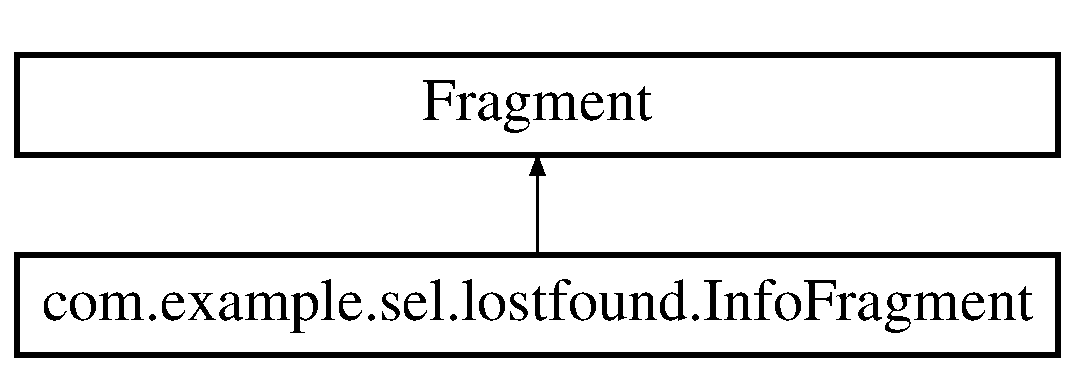
\includegraphics[height=2.000000cm]{classcom_1_1example_1_1sel_1_1lostfound_1_1InfoFragment}
\end{center}
\end{figure}
\subsection*{Classes}
\begin{DoxyCompactItemize}
\item 
interface \hyperlink{interfacecom_1_1example_1_1sel_1_1lostfound_1_1InfoFragment_1_1OnFragmentInteractionListener}{On\-Fragment\-Interaction\-Listener}
\end{DoxyCompactItemize}
\subsection*{Public Member Functions}
\begin{DoxyCompactItemize}
\item 
void \hyperlink{classcom_1_1example_1_1sel_1_1lostfound_1_1InfoFragment_a1a9382b4b0ceacfc464559a897fa7656}{on\-Create} (Bundle saved\-Instance\-State)
\begin{DoxyCompactList}\small\item\em on opening or selecting info fragment from navigation bar \end{DoxyCompactList}\item 
\hypertarget{classcom_1_1example_1_1sel_1_1lostfound_1_1InfoFragment_adb5e6a68883e5b4cb236e0e2e221d7f4}{View {\bfseries on\-Create\-View} (Layout\-Inflater inflater, View\-Group container, Bundle saved\-Instance\-State)}\label{classcom_1_1example_1_1sel_1_1lostfound_1_1InfoFragment_adb5e6a68883e5b4cb236e0e2e221d7f4}

\item 
\hypertarget{classcom_1_1example_1_1sel_1_1lostfound_1_1InfoFragment_a20ae678d3072262f318a083241372871}{void {\bfseries on\-Button\-Pressed} (Uri uri)}\label{classcom_1_1example_1_1sel_1_1lostfound_1_1InfoFragment_a20ae678d3072262f318a083241372871}

\item 
\hypertarget{classcom_1_1example_1_1sel_1_1lostfound_1_1InfoFragment_a07cb9a9ac26dec9f20abce73c04f92e1}{void {\bfseries on\-Attach} (Context context)}\label{classcom_1_1example_1_1sel_1_1lostfound_1_1InfoFragment_a07cb9a9ac26dec9f20abce73c04f92e1}

\item 
\hypertarget{classcom_1_1example_1_1sel_1_1lostfound_1_1InfoFragment_a1fff5a01de59e68f81999e2c558325ba}{void {\bfseries on\-Detach} ()}\label{classcom_1_1example_1_1sel_1_1lostfound_1_1InfoFragment_a1fff5a01de59e68f81999e2c558325ba}

\end{DoxyCompactItemize}
\subsection*{Static Public Member Functions}
\begin{DoxyCompactItemize}
\item 
static \hyperlink{classcom_1_1example_1_1sel_1_1lostfound_1_1InfoFragment}{Info\-Fragment} \hyperlink{classcom_1_1example_1_1sel_1_1lostfound_1_1InfoFragment_adb1e26f4f2a3a0f918bff5c5df58e695}{new\-Instance} (String param1, String param2)
\begin{DoxyCompactList}\small\item\em a constructor \end{DoxyCompactList}\end{DoxyCompactItemize}


\subsection{Detailed Description}
Created by Rohit G on 4/2/2016. A simple \hyperlink{}{Fragment} subclass. Activities that contain this fragment must implement the \hyperlink{interfacecom_1_1example_1_1sel_1_1lostfound_1_1InfoFragment_1_1OnFragmentInteractionListener}{Info\-Fragment.\-On\-Fragment\-Interaction\-Listener} interface to handle interaction events. Use the \hyperlink{classcom_1_1example_1_1sel_1_1lostfound_1_1InfoFragment_adb1e26f4f2a3a0f918bff5c5df58e695}{Info\-Fragment\#new\-Instance} factory method to create an instance of this fragment. A class implementing Help and F\-A\-Q fragment of navigation bar 

\subsection{Member Function Documentation}
\hypertarget{classcom_1_1example_1_1sel_1_1lostfound_1_1InfoFragment_adb1e26f4f2a3a0f918bff5c5df58e695}{\index{com\-::example\-::sel\-::lostfound\-::\-Info\-Fragment@{com\-::example\-::sel\-::lostfound\-::\-Info\-Fragment}!new\-Instance@{new\-Instance}}
\index{new\-Instance@{new\-Instance}!com::example::sel::lostfound::InfoFragment@{com\-::example\-::sel\-::lostfound\-::\-Info\-Fragment}}
\subsubsection[{new\-Instance}]{\setlength{\rightskip}{0pt plus 5cm}static {\bf Info\-Fragment} com.\-example.\-sel.\-lostfound.\-Info\-Fragment.\-new\-Instance (
\begin{DoxyParamCaption}
\item[{String}]{param1, }
\item[{String}]{param2}
\end{DoxyParamCaption}
)\hspace{0.3cm}{\ttfamily [inline]}, {\ttfamily [static]}}}\label{classcom_1_1example_1_1sel_1_1lostfound_1_1InfoFragment_adb1e26f4f2a3a0f918bff5c5df58e695}


a constructor 

Use this factory method to create a new instance of this fragment using the provided parameters.


\begin{DoxyParams}{Parameters}
{\em param1} & Parameter 1. \\
\hline
{\em param2} & Parameter 2. \\
\hline
\end{DoxyParams}
\begin{DoxyReturn}{Returns}
A new instance of fragment \hyperlink{classcom_1_1example_1_1sel_1_1lostfound_1_1InfoFragment}{Info\-Fragment}. 
\end{DoxyReturn}
\hypertarget{classcom_1_1example_1_1sel_1_1lostfound_1_1InfoFragment_a1a9382b4b0ceacfc464559a897fa7656}{\index{com\-::example\-::sel\-::lostfound\-::\-Info\-Fragment@{com\-::example\-::sel\-::lostfound\-::\-Info\-Fragment}!on\-Create@{on\-Create}}
\index{on\-Create@{on\-Create}!com::example::sel::lostfound::InfoFragment@{com\-::example\-::sel\-::lostfound\-::\-Info\-Fragment}}
\subsubsection[{on\-Create}]{\setlength{\rightskip}{0pt plus 5cm}void com.\-example.\-sel.\-lostfound.\-Info\-Fragment.\-on\-Create (
\begin{DoxyParamCaption}
\item[{Bundle}]{saved\-Instance\-State}
\end{DoxyParamCaption}
)\hspace{0.3cm}{\ttfamily [inline]}}}\label{classcom_1_1example_1_1sel_1_1lostfound_1_1InfoFragment_a1a9382b4b0ceacfc464559a897fa7656}


on opening or selecting info fragment from navigation bar 

$<$ Info action bar in navigation bar 

The documentation for this class was generated from the following file\-:\begin{DoxyCompactItemize}
\item 
Info\-Fragment.\-java\end{DoxyCompactItemize}

\hypertarget{classcom_1_1example_1_1sel_1_1lostfound_1_1MainActivity}{\section{com.\-example.\-sel.\-lostfound.\-Main\-Activity Class Reference}
\label{classcom_1_1example_1_1sel_1_1lostfound_1_1MainActivity}\index{com.\-example.\-sel.\-lostfound.\-Main\-Activity@{com.\-example.\-sel.\-lostfound.\-Main\-Activity}}
}


Main activity class.  


Inheritance diagram for com.\-example.\-sel.\-lostfound.\-Main\-Activity\-:\begin{figure}[H]
\begin{center}
\leavevmode
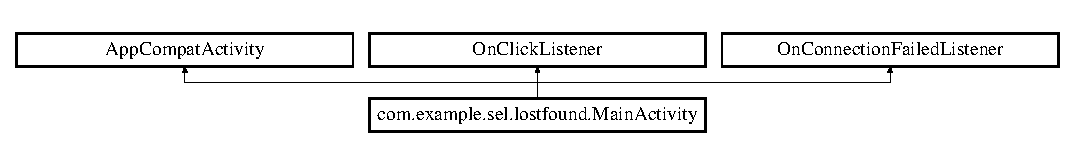
\includegraphics[height=1.542700cm]{classcom_1_1example_1_1sel_1_1lostfound_1_1MainActivity}
\end{center}
\end{figure}
\subsection*{Public Member Functions}
\begin{DoxyCompactItemize}
\item 
\hypertarget{classcom_1_1example_1_1sel_1_1lostfound_1_1MainActivity_a55b436bf176e21d22abf837dc8f2602c}{void \hyperlink{classcom_1_1example_1_1sel_1_1lostfound_1_1MainActivity_a55b436bf176e21d22abf837dc8f2602c}{is\-Signed\-In} ()}\label{classcom_1_1example_1_1sel_1_1lostfound_1_1MainActivity_a55b436bf176e21d22abf837dc8f2602c}

\begin{DoxyCompactList}\small\item\em function to sign in via google \end{DoxyCompactList}\item 
\hypertarget{classcom_1_1example_1_1sel_1_1lostfound_1_1MainActivity_af6914b0175f989ccb1c616f05a162f1a}{void \hyperlink{classcom_1_1example_1_1sel_1_1lostfound_1_1MainActivity_af6914b0175f989ccb1c616f05a162f1a}{continue\-Sign\-In} (View view)}\label{classcom_1_1example_1_1sel_1_1lostfound_1_1MainActivity_af6914b0175f989ccb1c616f05a162f1a}

\begin{DoxyCompactList}\small\item\em function to sign in into same account as previously signed in \end{DoxyCompactList}\item 
\hypertarget{classcom_1_1example_1_1sel_1_1lostfound_1_1MainActivity_a4618c5d451d4e0c2ce4562499a583ee5}{void \hyperlink{classcom_1_1example_1_1sel_1_1lostfound_1_1MainActivity_a4618c5d451d4e0c2ce4562499a583ee5}{proceed} (View view)}\label{classcom_1_1example_1_1sel_1_1lostfound_1_1MainActivity_a4618c5d451d4e0c2ce4562499a583ee5}

\begin{DoxyCompactList}\small\item\em function to proceed login after validating the email id entered \end{DoxyCompactList}\item 
\hypertarget{classcom_1_1example_1_1sel_1_1lostfound_1_1MainActivity_ac979afc8333ca7e81e7859cd383c614d}{void {\bfseries on\-Click} (View v)}\label{classcom_1_1example_1_1sel_1_1lostfound_1_1MainActivity_ac979afc8333ca7e81e7859cd383c614d}

\item 
\hypertarget{classcom_1_1example_1_1sel_1_1lostfound_1_1MainActivity_a15df38b4157a1f3a7c9dd7c8099e7495}{void \hyperlink{classcom_1_1example_1_1sel_1_1lostfound_1_1MainActivity_a15df38b4157a1f3a7c9dd7c8099e7495}{on\-Connection\-Failed} (Connection\-Result connection\-Result)}\label{classcom_1_1example_1_1sel_1_1lostfound_1_1MainActivity_a15df38b4157a1f3a7c9dd7c8099e7495}

\begin{DoxyCompactList}\small\item\em function on entering email id other than nitc email id \end{DoxyCompactList}\item 
\hypertarget{classcom_1_1example_1_1sel_1_1lostfound_1_1MainActivity_ad934ef9a9347dc67bcaf5365213f58da}{void {\bfseries on\-Activity\-Result} (int request\-Code, int result\-Code, Intent data)}\label{classcom_1_1example_1_1sel_1_1lostfound_1_1MainActivity_ad934ef9a9347dc67bcaf5365213f58da}

\end{DoxyCompactItemize}
\subsection*{Protected Member Functions}
\begin{DoxyCompactItemize}
\item 
\hypertarget{classcom_1_1example_1_1sel_1_1lostfound_1_1MainActivity_ac0ce1d56e609a8b69d6227c6d4d59f48}{void \hyperlink{classcom_1_1example_1_1sel_1_1lostfound_1_1MainActivity_ac0ce1d56e609a8b69d6227c6d4d59f48}{on\-Create} (Bundle saved\-Instance\-State)}\label{classcom_1_1example_1_1sel_1_1lostfound_1_1MainActivity_ac0ce1d56e609a8b69d6227c6d4d59f48}

\begin{DoxyCompactList}\small\item\em function implementing log in feature \end{DoxyCompactList}\end{DoxyCompactItemize}
\subsection*{Static Protected Attributes}
\begin{DoxyCompactItemize}
\item 
\hypertarget{classcom_1_1example_1_1sel_1_1lostfound_1_1MainActivity_a1a8d41b931cf85891f5fd3497d34a32a}{static String {\bfseries user\-Name}}\label{classcom_1_1example_1_1sel_1_1lostfound_1_1MainActivity_a1a8d41b931cf85891f5fd3497d34a32a}

\item 
\hypertarget{classcom_1_1example_1_1sel_1_1lostfound_1_1MainActivity_a02198420522a5b05dbc3202b74dd9a59}{static String {\bfseries user\-Email}}\label{classcom_1_1example_1_1sel_1_1lostfound_1_1MainActivity_a02198420522a5b05dbc3202b74dd9a59}

\item 
\hypertarget{classcom_1_1example_1_1sel_1_1lostfound_1_1MainActivity_a92248fd7e13b4972f457ad9791ba253c}{static Uri {\bfseries user\-Image}}\label{classcom_1_1example_1_1sel_1_1lostfound_1_1MainActivity_a92248fd7e13b4972f457ad9791ba253c}

\end{DoxyCompactItemize}


\subsection{Detailed Description}
Main activity class. 

implementing authentication of email id and log-\/in 

The documentation for this class was generated from the following file\-:\begin{DoxyCompactItemize}
\item 
Main\-Activity.\-java\end{DoxyCompactItemize}

<<<<<<< HEAD
\hypertarget{interfacecom_1_1example_1_1sel_1_1lostfound_1_1InfoFragment_1_1OnFragmentInteractionListener}{\section{com.\-example.\-sel.\-lostfound.\-Info\-Fragment.\-On\-Fragment\-Interaction\-Listener Interface Reference}
\label{interfacecom_1_1example_1_1sel_1_1lostfound_1_1InfoFragment_1_1OnFragmentInteractionListener}\index{com.\-example.\-sel.\-lostfound.\-Info\-Fragment.\-On\-Fragment\-Interaction\-Listener@{com.\-example.\-sel.\-lostfound.\-Info\-Fragment.\-On\-Fragment\-Interaction\-Listener}}
}
Inheritance diagram for com.\-example.\-sel.\-lostfound.\-Info\-Fragment.\-On\-Fragment\-Interaction\-Listener\-:\begin{figure}[H]
=======
\hypertarget{interfacecom_1_1example_1_1sel_1_1lostfound_1_1InfoFragment_1_1OnFragmentInteractionListener}{\section{com.\-example.\-sel.\-lostfound.\-Info\-Fragment.\-On\-Fragment\-Interaction\-Listener \-Interface \-Reference}
\label{interfacecom_1_1example_1_1sel_1_1lostfound_1_1InfoFragment_1_1OnFragmentInteractionListener}\index{com.\-example.\-sel.\-lostfound.\-Info\-Fragment.\-On\-Fragment\-Interaction\-Listener@{com.\-example.\-sel.\-lostfound.\-Info\-Fragment.\-On\-Fragment\-Interaction\-Listener}}
}
\-Inheritance diagram for com.\-example.\-sel.\-lostfound.\-Info\-Fragment.\-On\-Fragment\-Interaction\-Listener\-:\begin{figure}[H]
>>>>>>> 0bbb2bc5f31f033d772ef4573f66c50564006509
\begin{center}
\leavevmode
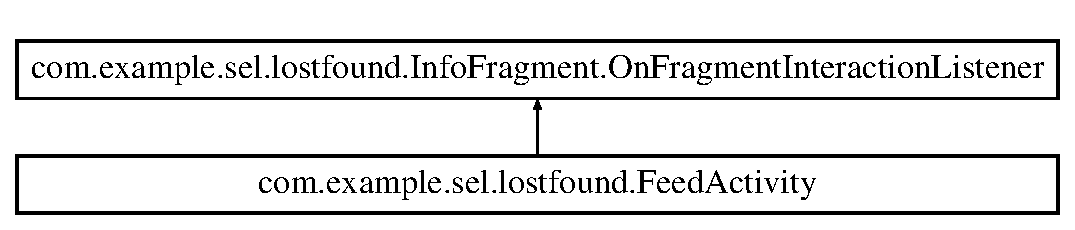
\includegraphics[height=2.000000cm]{interfacecom_1_1example_1_1sel_1_1lostfound_1_1InfoFragment_1_1OnFragmentInteractionListener}
\end{center}
\end{figure}
<<<<<<< HEAD
\subsection*{Public Member Functions}
\begin{DoxyCompactItemize}
\item 
\hypertarget{interfacecom_1_1example_1_1sel_1_1lostfound_1_1InfoFragment_1_1OnFragmentInteractionListener_a6aa219ac44d543de0564fc4d60ddb055}{void {\bfseries on\-Info\-Fragment\-Interaction} (String string)}\label{interfacecom_1_1example_1_1sel_1_1lostfound_1_1InfoFragment_1_1OnFragmentInteractionListener_a6aa219ac44d543de0564fc4d60ddb055}

\item 
\hypertarget{interfacecom_1_1example_1_1sel_1_1lostfound_1_1InfoFragment_1_1OnFragmentInteractionListener_aaee7dd0f88da8e1ff9c1213285377017}{void {\bfseries on\-Fragment\-Interaction} (Uri uri)}\label{interfacecom_1_1example_1_1sel_1_1lostfound_1_1InfoFragment_1_1OnFragmentInteractionListener_aaee7dd0f88da8e1ff9c1213285377017}
=======
\subsection*{\-Public \-Member \-Functions}
\begin{DoxyCompactItemize}
\item 
\hypertarget{interfacecom_1_1example_1_1sel_1_1lostfound_1_1InfoFragment_1_1OnFragmentInteractionListener_a6aa219ac44d543de0564fc4d60ddb055}{void {\bfseries on\-Info\-Fragment\-Interaction} (\-String string)}\label{interfacecom_1_1example_1_1sel_1_1lostfound_1_1InfoFragment_1_1OnFragmentInteractionListener_a6aa219ac44d543de0564fc4d60ddb055}

\item 
\hypertarget{interfacecom_1_1example_1_1sel_1_1lostfound_1_1InfoFragment_1_1OnFragmentInteractionListener_aaee7dd0f88da8e1ff9c1213285377017}{void {\bfseries on\-Fragment\-Interaction} (\-Uri uri)}\label{interfacecom_1_1example_1_1sel_1_1lostfound_1_1InfoFragment_1_1OnFragmentInteractionListener_aaee7dd0f88da8e1ff9c1213285377017}
>>>>>>> 0bbb2bc5f31f033d772ef4573f66c50564006509

\end{DoxyCompactItemize}


<<<<<<< HEAD
\subsection{Detailed Description}
This interface must be implemented by activities that contain this fragment to allow an interaction in this fragment to be communicated to the activity and potentially other fragments contained in that activity. 

See the Android Training lesson \href{http://developer.android.com/training/basics/fragments/communicating.html}{\tt Communicating with Other Fragments} for more information. 

The documentation for this interface was generated from the following file\-:\begin{DoxyCompactItemize}
\item 
Info\-Fragment.\-java\end{DoxyCompactItemize}
=======
\subsection{\-Detailed \-Description}
\-This interface must be implemented by activities that contain this fragment to allow an interaction in this fragment to be communicated to the activity and potentially other fragments contained in that activity. 

\-See the \-Android \-Training lesson \href{http://developer.android.com/training/basics/fragments/communicating.html}{\tt \-Communicating with \-Other \-Fragments} for more information. 

\-The documentation for this interface was generated from the following file\-:\begin{DoxyCompactItemize}
\item 
\-Info\-Fragment.\-java\end{DoxyCompactItemize}
>>>>>>> 0bbb2bc5f31f033d772ef4573f66c50564006509

<<<<<<< HEAD
\hypertarget{interfacecom_1_1example_1_1sel_1_1lostfound_1_1ProfileFragment_1_1OnFragmentInteractionListener}{\section{com.\-example.\-sel.\-lostfound.\-Profile\-Fragment.\-On\-Fragment\-Interaction\-Listener Interface Reference}
\label{interfacecom_1_1example_1_1sel_1_1lostfound_1_1ProfileFragment_1_1OnFragmentInteractionListener}\index{com.\-example.\-sel.\-lostfound.\-Profile\-Fragment.\-On\-Fragment\-Interaction\-Listener@{com.\-example.\-sel.\-lostfound.\-Profile\-Fragment.\-On\-Fragment\-Interaction\-Listener}}
}
Inheritance diagram for com.\-example.\-sel.\-lostfound.\-Profile\-Fragment.\-On\-Fragment\-Interaction\-Listener\-:\begin{figure}[H]
=======
\hypertarget{interfacecom_1_1example_1_1sel_1_1lostfound_1_1ProfileFragment_1_1OnFragmentInteractionListener}{\section{com.\-example.\-sel.\-lostfound.\-Profile\-Fragment.\-On\-Fragment\-Interaction\-Listener \-Interface \-Reference}
\label{interfacecom_1_1example_1_1sel_1_1lostfound_1_1ProfileFragment_1_1OnFragmentInteractionListener}\index{com.\-example.\-sel.\-lostfound.\-Profile\-Fragment.\-On\-Fragment\-Interaction\-Listener@{com.\-example.\-sel.\-lostfound.\-Profile\-Fragment.\-On\-Fragment\-Interaction\-Listener}}
}
\-Inheritance diagram for com.\-example.\-sel.\-lostfound.\-Profile\-Fragment.\-On\-Fragment\-Interaction\-Listener\-:\begin{figure}[H]
>>>>>>> 0bbb2bc5f31f033d772ef4573f66c50564006509
\begin{center}
\leavevmode
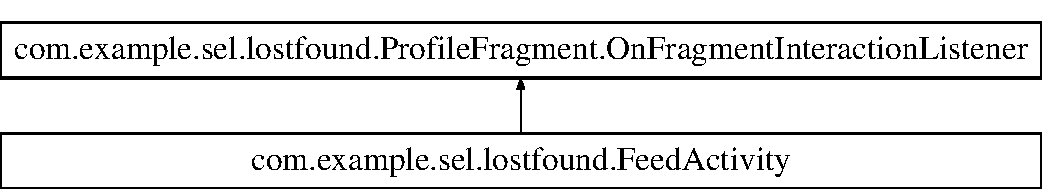
\includegraphics[height=2.000000cm]{interfacecom_1_1example_1_1sel_1_1lostfound_1_1ProfileFragment_1_1OnFragmentInteractionListener}
\end{center}
\end{figure}
<<<<<<< HEAD
\subsection*{Public Member Functions}
\begin{DoxyCompactItemize}
\item 
\hypertarget{interfacecom_1_1example_1_1sel_1_1lostfound_1_1ProfileFragment_1_1OnFragmentInteractionListener_af75f735b544a4f6c22f58e2f0ea5c671}{void {\bfseries on\-Profile\-Fragment\-Interaction} (String string)}\label{interfacecom_1_1example_1_1sel_1_1lostfound_1_1ProfileFragment_1_1OnFragmentInteractionListener_af75f735b544a4f6c22f58e2f0ea5c671}

\item 
\hypertarget{interfacecom_1_1example_1_1sel_1_1lostfound_1_1ProfileFragment_1_1OnFragmentInteractionListener_acde287647e7b1caa72e45c54814c5e3f}{void {\bfseries on\-Fragment\-Interaction} (Uri uri)}\label{interfacecom_1_1example_1_1sel_1_1lostfound_1_1ProfileFragment_1_1OnFragmentInteractionListener_acde287647e7b1caa72e45c54814c5e3f}
=======
\subsection*{\-Public \-Member \-Functions}
\begin{DoxyCompactItemize}
\item 
\hypertarget{interfacecom_1_1example_1_1sel_1_1lostfound_1_1ProfileFragment_1_1OnFragmentInteractionListener_af75f735b544a4f6c22f58e2f0ea5c671}{void {\bfseries on\-Profile\-Fragment\-Interaction} (\-String string)}\label{interfacecom_1_1example_1_1sel_1_1lostfound_1_1ProfileFragment_1_1OnFragmentInteractionListener_af75f735b544a4f6c22f58e2f0ea5c671}

\item 
\hypertarget{interfacecom_1_1example_1_1sel_1_1lostfound_1_1ProfileFragment_1_1OnFragmentInteractionListener_acde287647e7b1caa72e45c54814c5e3f}{void {\bfseries on\-Fragment\-Interaction} (\-Uri uri)}\label{interfacecom_1_1example_1_1sel_1_1lostfound_1_1ProfileFragment_1_1OnFragmentInteractionListener_acde287647e7b1caa72e45c54814c5e3f}
>>>>>>> 0bbb2bc5f31f033d772ef4573f66c50564006509

\end{DoxyCompactItemize}


<<<<<<< HEAD
\subsection{Detailed Description}
This interface must be implemented by activities that contain this fragment to allow an interaction in this fragment to be communicated to the activity and potentially other fragments contained in that activity. 

See the Android Training lesson \href{http://developer.android.com/training/basics/fragments/communicating.html}{\tt Communicating with Other Fragments} for more information. 

The documentation for this interface was generated from the following file\-:\begin{DoxyCompactItemize}
\item 
Profile\-Fragment.\-java\end{DoxyCompactItemize}
=======
\subsection{\-Detailed \-Description}
\-This interface must be implemented by activities that contain this fragment to allow an interaction in this fragment to be communicated to the activity and potentially other fragments contained in that activity. 

\-See the \-Android \-Training lesson \href{http://developer.android.com/training/basics/fragments/communicating.html}{\tt \-Communicating with \-Other \-Fragments} for more information. 

\-The documentation for this interface was generated from the following file\-:\begin{DoxyCompactItemize}
\item 
\-Profile\-Fragment.\-java\end{DoxyCompactItemize}
>>>>>>> 0bbb2bc5f31f033d772ef4573f66c50564006509

\hypertarget{interfacecom_1_1example_1_1sel_1_1lostfound_1_1FeedFragment_1_1OnFragmentInteractionListener}{\section{com.\-example.\-sel.\-lostfound.\-Feed\-Fragment.\-On\-Fragment\-Interaction\-Listener \-Interface \-Reference}
\label{interfacecom_1_1example_1_1sel_1_1lostfound_1_1FeedFragment_1_1OnFragmentInteractionListener}\index{com.\-example.\-sel.\-lostfound.\-Feed\-Fragment.\-On\-Fragment\-Interaction\-Listener@{com.\-example.\-sel.\-lostfound.\-Feed\-Fragment.\-On\-Fragment\-Interaction\-Listener}}
}
\-Inheritance diagram for com.\-example.\-sel.\-lostfound.\-Feed\-Fragment.\-On\-Fragment\-Interaction\-Listener\-:\begin{figure}[H]
\begin{center}
\leavevmode
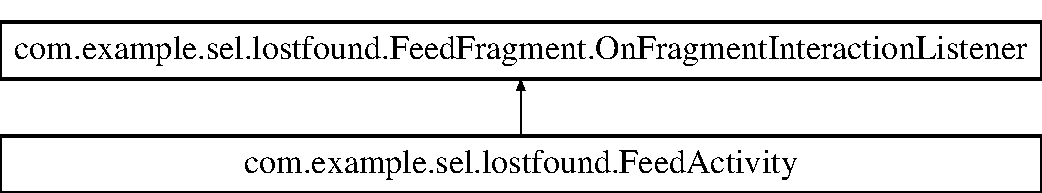
\includegraphics[height=2.000000cm]{interfacecom_1_1example_1_1sel_1_1lostfound_1_1FeedFragment_1_1OnFragmentInteractionListener}
\end{center}
\end{figure}
\subsection*{\-Public \-Member \-Functions}
\begin{DoxyCompactItemize}
\item 
\hypertarget{interfacecom_1_1example_1_1sel_1_1lostfound_1_1FeedFragment_1_1OnFragmentInteractionListener_a147ba47e242fae7f6095d672ab95d18a}{void {\bfseries on\-Feed\-Fragment\-Interaction} (\-String string)}\label{interfacecom_1_1example_1_1sel_1_1lostfound_1_1FeedFragment_1_1OnFragmentInteractionListener_a147ba47e242fae7f6095d672ab95d18a}

\item 
\hypertarget{interfacecom_1_1example_1_1sel_1_1lostfound_1_1FeedFragment_1_1OnFragmentInteractionListener_aeada926fa0dcf59d4b17dbe757d198ee}{void {\bfseries on\-Fragment\-Interaction} (\-Uri uri)}\label{interfacecom_1_1example_1_1sel_1_1lostfound_1_1FeedFragment_1_1OnFragmentInteractionListener_aeada926fa0dcf59d4b17dbe757d198ee}

\end{DoxyCompactItemize}


\subsection{\-Detailed \-Description}
\-This interface must be implemented by activities that contain this fragment to allow an interaction in this fragment to be communicated to the activity and potentially other fragments contained in that activity. 

\-See the \-Android \-Training lesson \href{http://developer.android.com/training/basics/fragments/communicating.html}{\tt \-Communicating with \-Other \-Fragments} for more information. 

\-The documentation for this interface was generated from the following file\-:\begin{DoxyCompactItemize}
\item 
\-Feed\-Fragment.\-java\end{DoxyCompactItemize}

\hypertarget{interfacecom_1_1example_1_1sel_1_1lostfound_1_1SubscribeFragment_1_1OnFragmentInteractionListener}{}\section{com.\+example.\+sel.\+lostfound.\+Subscribe\+Fragment.\+On\+Fragment\+Interaction\+Listener Interface Reference}
\label{interfacecom_1_1example_1_1sel_1_1lostfound_1_1SubscribeFragment_1_1OnFragmentInteractionListener}\index{com.\+example.\+sel.\+lostfound.\+Subscribe\+Fragment.\+On\+Fragment\+Interaction\+Listener@{com.\+example.\+sel.\+lostfound.\+Subscribe\+Fragment.\+On\+Fragment\+Interaction\+Listener}}
Inheritance diagram for com.\+example.\+sel.\+lostfound.\+Subscribe\+Fragment.\+On\+Fragment\+Interaction\+Listener\+:\begin{figure}[H]
\begin{center}
\leavevmode
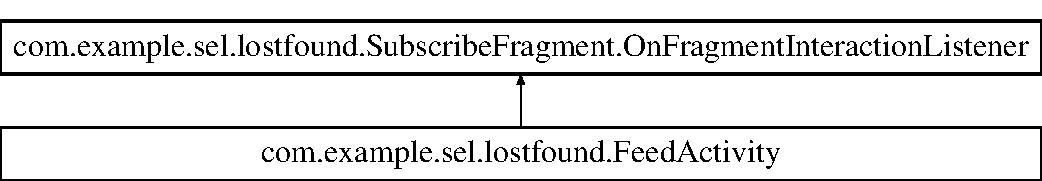
\includegraphics[height=2.000000cm]{interfacecom_1_1example_1_1sel_1_1lostfound_1_1SubscribeFragment_1_1OnFragmentInteractionListener}
\end{center}
\end{figure}
\subsection*{Public Member Functions}
\begin{DoxyCompactItemize}
\item 
void {\bfseries on\+Subscribe\+Fragment\+Interaction} (String string)\hypertarget{interfacecom_1_1example_1_1sel_1_1lostfound_1_1SubscribeFragment_1_1OnFragmentInteractionListener_a49e52bf52ac045228eda481eaa5ad3a3}{}\label{interfacecom_1_1example_1_1sel_1_1lostfound_1_1SubscribeFragment_1_1OnFragmentInteractionListener_a49e52bf52ac045228eda481eaa5ad3a3}

\item 
void {\bfseries on\+Fragment\+Interaction} (Uri uri)\hypertarget{interfacecom_1_1example_1_1sel_1_1lostfound_1_1SubscribeFragment_1_1OnFragmentInteractionListener_a419de726f221023d20f573225984783b}{}\label{interfacecom_1_1example_1_1sel_1_1lostfound_1_1SubscribeFragment_1_1OnFragmentInteractionListener_a419de726f221023d20f573225984783b}

\end{DoxyCompactItemize}


\subsection{Detailed Description}
This interface must be implemented by activities that contain this fragment to allow an interaction in this fragment to be communicated to the activity and potentially other fragments contained in that activity. 

See the Android Training lesson \href{http://developer.android.com/training/basics/fragments/communicating.html}{\tt Communicating with Other Fragments} for more information. 

The documentation for this interface was generated from the following file\+:\begin{DoxyCompactItemize}
\item 
Subscribe\+Fragment.\+java\end{DoxyCompactItemize}

<<<<<<< HEAD
\hypertarget{interfacecom_1_1example_1_1sel_1_1lostfound_1_1PostFragment_1_1OnFragmentInteractionListener}{\section{com.\-example.\-sel.\-lostfound.\-Post\-Fragment.\-On\-Fragment\-Interaction\-Listener Interface Reference}
\label{interfacecom_1_1example_1_1sel_1_1lostfound_1_1PostFragment_1_1OnFragmentInteractionListener}\index{com.\-example.\-sel.\-lostfound.\-Post\-Fragment.\-On\-Fragment\-Interaction\-Listener@{com.\-example.\-sel.\-lostfound.\-Post\-Fragment.\-On\-Fragment\-Interaction\-Listener}}
}
Inheritance diagram for com.\-example.\-sel.\-lostfound.\-Post\-Fragment.\-On\-Fragment\-Interaction\-Listener\-:\begin{figure}[H]
=======
\hypertarget{interfacecom_1_1example_1_1sel_1_1lostfound_1_1PostFragment_1_1OnFragmentInteractionListener}{\section{com.\-example.\-sel.\-lostfound.\-Post\-Fragment.\-On\-Fragment\-Interaction\-Listener \-Interface \-Reference}
\label{interfacecom_1_1example_1_1sel_1_1lostfound_1_1PostFragment_1_1OnFragmentInteractionListener}\index{com.\-example.\-sel.\-lostfound.\-Post\-Fragment.\-On\-Fragment\-Interaction\-Listener@{com.\-example.\-sel.\-lostfound.\-Post\-Fragment.\-On\-Fragment\-Interaction\-Listener}}
}
\-Inheritance diagram for com.\-example.\-sel.\-lostfound.\-Post\-Fragment.\-On\-Fragment\-Interaction\-Listener\-:\begin{figure}[H]
>>>>>>> 0bbb2bc5f31f033d772ef4573f66c50564006509
\begin{center}
\leavevmode
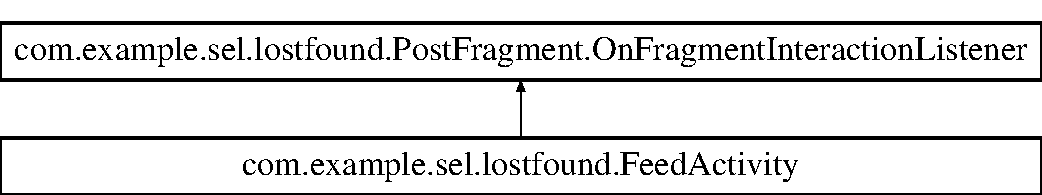
\includegraphics[height=2.000000cm]{interfacecom_1_1example_1_1sel_1_1lostfound_1_1PostFragment_1_1OnFragmentInteractionListener}
\end{center}
\end{figure}
<<<<<<< HEAD
\subsection*{Public Member Functions}
\begin{DoxyCompactItemize}
\item 
\hypertarget{interfacecom_1_1example_1_1sel_1_1lostfound_1_1PostFragment_1_1OnFragmentInteractionListener_a9ca2bef2b5bd8c3f86dd3e8f14045b17}{void {\bfseries on\-Post\-Fragment\-Interaction} (String string)}\label{interfacecom_1_1example_1_1sel_1_1lostfound_1_1PostFragment_1_1OnFragmentInteractionListener_a9ca2bef2b5bd8c3f86dd3e8f14045b17}

\item 
\hypertarget{interfacecom_1_1example_1_1sel_1_1lostfound_1_1PostFragment_1_1OnFragmentInteractionListener_a1fd1f1bbc8912c5d04c708869645dc8e}{void {\bfseries on\-Fragment\-Interaction} (Uri uri)}\label{interfacecom_1_1example_1_1sel_1_1lostfound_1_1PostFragment_1_1OnFragmentInteractionListener_a1fd1f1bbc8912c5d04c708869645dc8e}
=======
\subsection*{\-Public \-Member \-Functions}
\begin{DoxyCompactItemize}
\item 
\hypertarget{interfacecom_1_1example_1_1sel_1_1lostfound_1_1PostFragment_1_1OnFragmentInteractionListener_a9ca2bef2b5bd8c3f86dd3e8f14045b17}{void {\bfseries on\-Post\-Fragment\-Interaction} (\-String string)}\label{interfacecom_1_1example_1_1sel_1_1lostfound_1_1PostFragment_1_1OnFragmentInteractionListener_a9ca2bef2b5bd8c3f86dd3e8f14045b17}

\item 
\hypertarget{interfacecom_1_1example_1_1sel_1_1lostfound_1_1PostFragment_1_1OnFragmentInteractionListener_a1fd1f1bbc8912c5d04c708869645dc8e}{void {\bfseries on\-Fragment\-Interaction} (\-Uri uri)}\label{interfacecom_1_1example_1_1sel_1_1lostfound_1_1PostFragment_1_1OnFragmentInteractionListener_a1fd1f1bbc8912c5d04c708869645dc8e}
>>>>>>> 0bbb2bc5f31f033d772ef4573f66c50564006509

\end{DoxyCompactItemize}


<<<<<<< HEAD
\subsection{Detailed Description}
This interface must be implemented by activities that contain this fragment to allow an interaction in this fragment to be communicated to the activity and potentially other fragments contained in that activity. 

See the Android Training lesson \href{http://developer.android.com/training/basics/fragments/communicating.html}{\tt Communicating with Other Fragments} for more information. 

The documentation for this interface was generated from the following file\-:\begin{DoxyCompactItemize}
\item 
Post\-Fragment.\-java\end{DoxyCompactItemize}
=======
\subsection{\-Detailed \-Description}
\-This interface must be implemented by activities that contain this fragment to allow an interaction in this fragment to be communicated to the activity and potentially other fragments contained in that activity. 

\-See the \-Android \-Training lesson \href{http://developer.android.com/training/basics/fragments/communicating.html}{\tt \-Communicating with \-Other \-Fragments} for more information. 

\-The documentation for this interface was generated from the following file\-:\begin{DoxyCompactItemize}
\item 
\-Post\-Fragment.\-java\end{DoxyCompactItemize}
>>>>>>> 0bbb2bc5f31f033d772ef4573f66c50564006509

\hypertarget{classcom_1_1example_1_1sel_1_1lostfound_1_1PostAdapter}{}\section{com.\+example.\+sel.\+lostfound.\+Post\+Adapter Class Reference}
\label{classcom_1_1example_1_1sel_1_1lostfound_1_1PostAdapter}\index{com.\+example.\+sel.\+lostfound.\+Post\+Adapter@{com.\+example.\+sel.\+lostfound.\+Post\+Adapter}}


A class implementing functions to get data from web server and implements report use-\/case.  


Inheritance diagram for com.\+example.\+sel.\+lostfound.\+Post\+Adapter\+:\begin{figure}[H]
\begin{center}
\leavevmode
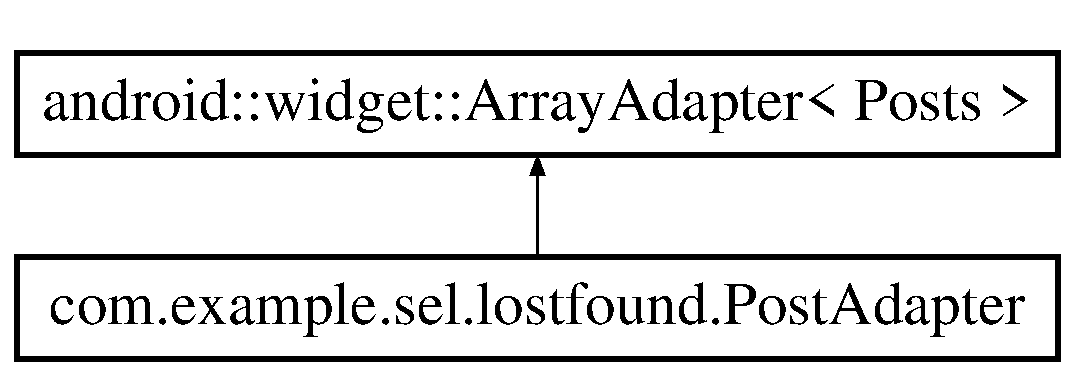
\includegraphics[height=2.000000cm]{classcom_1_1example_1_1sel_1_1lostfound_1_1PostAdapter}
\end{center}
\end{figure}
\subsection*{Classes}
\begin{DoxyCompactItemize}
\item 
class {\bfseries Post\+Holder}
\end{DoxyCompactItemize}
\subsection*{Public Member Functions}
\begin{DoxyCompactItemize}
\item 
\hyperlink{classcom_1_1example_1_1sel_1_1lostfound_1_1PostAdapter_a58de5e8d3132dd70bfd35dcb44bf80e1}{Post\+Adapter} (Context context, int resource, List$<$ \hyperlink{classcom_1_1example_1_1sel_1_1lostfound_1_1Posts}{Posts} $>$ posts)\hypertarget{classcom_1_1example_1_1sel_1_1lostfound_1_1PostAdapter_a58de5e8d3132dd70bfd35dcb44bf80e1}{}\label{classcom_1_1example_1_1sel_1_1lostfound_1_1PostAdapter_a58de5e8d3132dd70bfd35dcb44bf80e1}

\begin{DoxyCompactList}\small\item\em a constructor \end{DoxyCompactList}\item 
View \hyperlink{classcom_1_1example_1_1sel_1_1lostfound_1_1PostAdapter_aa2f3c1364857d97091ba325de3df6226}{get\+View} (int position, View convert\+View, View\+Group parent)
\begin{DoxyCompactList}\small\item\em implementing list view of posts \end{DoxyCompactList}\end{DoxyCompactItemize}


\subsection{Detailed Description}
A class implementing functions to get data from web server and implements report use-\/case. 

Created by achu on 09-\/04-\/2016. 

\subsection{Member Function Documentation}
\index{com\+::example\+::sel\+::lostfound\+::\+Post\+Adapter@{com\+::example\+::sel\+::lostfound\+::\+Post\+Adapter}!get\+View@{get\+View}}
\index{get\+View@{get\+View}!com\+::example\+::sel\+::lostfound\+::\+Post\+Adapter@{com\+::example\+::sel\+::lostfound\+::\+Post\+Adapter}}
\subsubsection[{\texorpdfstring{get\+View(int position, View convert\+View, View\+Group parent)}{getView(int position, View convertView, ViewGroup parent)}}]{\setlength{\rightskip}{0pt plus 5cm}View com.\+example.\+sel.\+lostfound.\+Post\+Adapter.\+get\+View (
\begin{DoxyParamCaption}
\item[{int}]{position, }
\item[{View}]{convert\+View, }
\item[{View\+Group}]{parent}
\end{DoxyParamCaption}
)\hspace{0.3cm}{\ttfamily [inline]}}\hypertarget{classcom_1_1example_1_1sel_1_1lostfound_1_1PostAdapter_aa2f3c1364857d97091ba325de3df6226}{}\label{classcom_1_1example_1_1sel_1_1lostfound_1_1PostAdapter_aa2f3c1364857d97091ba325de3df6226}


implementing list view of posts 

reported(reported more than thrice) posts

display posts in list format

$<$ contact button to contact the author

function to implement action on clicking contact button

new page directed consisting of compose email

report button implementation

function to update report count in database in webserver

server response via On\+Post\+Execute function 

The documentation for this class was generated from the following file\+:\begin{DoxyCompactItemize}
\item 
Post\+Adapter.\+java\end{DoxyCompactItemize}

\hypertarget{classcom_1_1example_1_1sel_1_1lostfound_1_1PostFragment}{}\section{com.\+example.\+sel.\+lostfound.\+Post\+Fragment Class Reference}
\label{classcom_1_1example_1_1sel_1_1lostfound_1_1PostFragment}\index{com.\+example.\+sel.\+lostfound.\+Post\+Fragment@{com.\+example.\+sel.\+lostfound.\+Post\+Fragment}}
Inheritance diagram for com.\+example.\+sel.\+lostfound.\+Post\+Fragment\+:\begin{figure}[H]
\begin{center}
\leavevmode
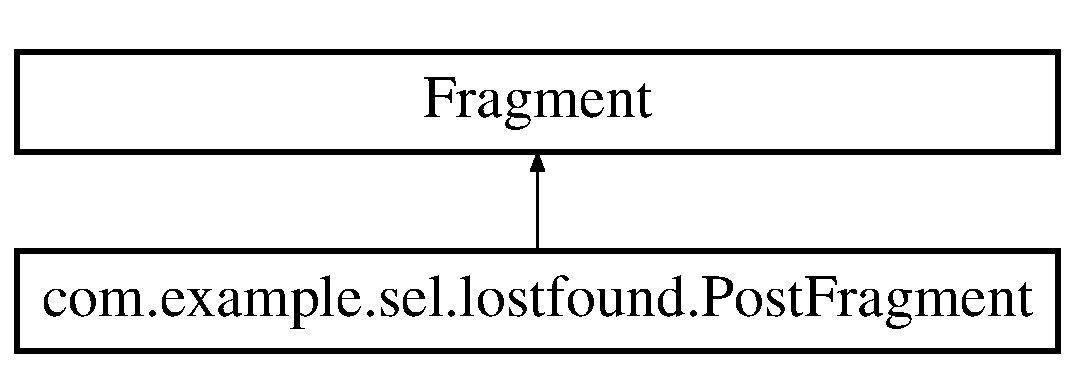
\includegraphics[height=2.000000cm]{classcom_1_1example_1_1sel_1_1lostfound_1_1PostFragment}
\end{center}
\end{figure}
\subsection*{Classes}
\begin{DoxyCompactItemize}
\item 
class {\bfseries Date\+Picker\+Fragment}
\begin{DoxyCompactList}\small\item\em a class implementing date picker \end{DoxyCompactList}\item 
interface \hyperlink{interfacecom_1_1example_1_1sel_1_1lostfound_1_1PostFragment_1_1OnFragmentInteractionListener}{On\+Fragment\+Interaction\+Listener}
\item 
class {\bfseries Time\+Picker\+Fragment}
\begin{DoxyCompactList}\small\item\em A class implementing time picker. \end{DoxyCompactList}\end{DoxyCompactItemize}
\subsection*{Public Member Functions}
\begin{DoxyCompactItemize}
\item 
void \hyperlink{classcom_1_1example_1_1sel_1_1lostfound_1_1PostFragment_a6ae53f1d4250edd39b3fab572b34a03c}{on\+Create} (Bundle saved\+Instance\+State)\hypertarget{classcom_1_1example_1_1sel_1_1lostfound_1_1PostFragment_a6ae53f1d4250edd39b3fab572b34a03c}{}\label{classcom_1_1example_1_1sel_1_1lostfound_1_1PostFragment_a6ae53f1d4250edd39b3fab572b34a03c}

\begin{DoxyCompactList}\small\item\em functions to be done after opening new instance of post fragment. \end{DoxyCompactList}\item 
View \hyperlink{classcom_1_1example_1_1sel_1_1lostfound_1_1PostFragment_a8c10184073835d28affa07720db256a4}{on\+Create\+View} (Layout\+Inflater inflater, View\+Group container, Bundle saved\+Instance\+State)
\begin{DoxyCompactList}\small\item\em function implementing task of extracting input by user into database \end{DoxyCompactList}\item 
void {\bfseries on\+Button\+Pressed} (Uri uri)\hypertarget{classcom_1_1example_1_1sel_1_1lostfound_1_1PostFragment_afba287683734ca9acaea52278c3e1eb5}{}\label{classcom_1_1example_1_1sel_1_1lostfound_1_1PostFragment_afba287683734ca9acaea52278c3e1eb5}

\item 
void {\bfseries on\+Attach} (Context context)\hypertarget{classcom_1_1example_1_1sel_1_1lostfound_1_1PostFragment_af8646c233bb3c70dbb6352f8a1c60e62}{}\label{classcom_1_1example_1_1sel_1_1lostfound_1_1PostFragment_af8646c233bb3c70dbb6352f8a1c60e62}

\item 
void {\bfseries on\+Detach} ()\hypertarget{classcom_1_1example_1_1sel_1_1lostfound_1_1PostFragment_ae96f353335b113be26870d00d3ac3b1c}{}\label{classcom_1_1example_1_1sel_1_1lostfound_1_1PostFragment_ae96f353335b113be26870d00d3ac3b1c}

\end{DoxyCompactItemize}
\subsection*{Static Public Member Functions}
\begin{DoxyCompactItemize}
\item 
static \hyperlink{classcom_1_1example_1_1sel_1_1lostfound_1_1PostFragment}{Post\+Fragment} \hyperlink{classcom_1_1example_1_1sel_1_1lostfound_1_1PostFragment_a7350f5b81aa9144d9acdeca902676773}{new\+Instance} (String param1, String param2)
\end{DoxyCompactItemize}
\subsection*{Static Public Attributes}
\begin{DoxyCompactItemize}
\item 
static Text\+View \hyperlink{classcom_1_1example_1_1sel_1_1lostfound_1_1PostFragment_ac6d98a5b689bea76cf1248a20a54d23c}{time\+Picker}
\item 
static Text\+View \hyperlink{classcom_1_1example_1_1sel_1_1lostfound_1_1PostFragment_a1c187b07da5262cf568439018a826ef9}{date\+Picker}
\end{DoxyCompactItemize}
\subsection*{Static Protected Attributes}
\begin{DoxyCompactItemize}
\item 
static String {\bfseries post\+Type} = \char`\"{}\char`\"{}\hypertarget{classcom_1_1example_1_1sel_1_1lostfound_1_1PostFragment_acb0672afa2382233136ee251bef7149b}{}\label{classcom_1_1example_1_1sel_1_1lostfound_1_1PostFragment_acb0672afa2382233136ee251bef7149b}

\item 
static Button \hyperlink{classcom_1_1example_1_1sel_1_1lostfound_1_1PostFragment_ab2d93225b515c22ccd209e1382e1a4a1}{post\+Button}
\end{DoxyCompactItemize}


\subsection{Detailed Description}
Created by Rohit G on 4/2/2016. A simple \hyperlink{}{Fragment} subclass. Activities that contain this fragment must implement the \hyperlink{interfacecom_1_1example_1_1sel_1_1lostfound_1_1PostFragment_1_1OnFragmentInteractionListener}{Post\+Fragment.\+On\+Fragment\+Interaction\+Listener} interface to handle interaction events. Use the \hyperlink{classcom_1_1example_1_1sel_1_1lostfound_1_1PostFragment_a7350f5b81aa9144d9acdeca902676773}{Post\+Fragment\#new\+Instance} factory method to create an instance of this fragment. class implementing post page 

\subsection{Member Function Documentation}
\index{com\+::example\+::sel\+::lostfound\+::\+Post\+Fragment@{com\+::example\+::sel\+::lostfound\+::\+Post\+Fragment}!new\+Instance@{new\+Instance}}
\index{new\+Instance@{new\+Instance}!com\+::example\+::sel\+::lostfound\+::\+Post\+Fragment@{com\+::example\+::sel\+::lostfound\+::\+Post\+Fragment}}
\subsubsection[{\texorpdfstring{new\+Instance(\+String param1, String param2)}{newInstance(String param1, String param2)}}]{\setlength{\rightskip}{0pt plus 5cm}static {\bf Post\+Fragment} com.\+example.\+sel.\+lostfound.\+Post\+Fragment.\+new\+Instance (
\begin{DoxyParamCaption}
\item[{String}]{param1, }
\item[{String}]{param2}
\end{DoxyParamCaption}
)\hspace{0.3cm}{\ttfamily [inline]}, {\ttfamily [static]}}\hypertarget{classcom_1_1example_1_1sel_1_1lostfound_1_1PostFragment_a7350f5b81aa9144d9acdeca902676773}{}\label{classcom_1_1example_1_1sel_1_1lostfound_1_1PostFragment_a7350f5b81aa9144d9acdeca902676773}
Use this factory method to create a new instance of this fragment using the provided parameters.


\begin{DoxyParams}{Parameters}
{\em param1} & Parameter 1. \\
\hline
{\em param2} & Parameter 2. \\
\hline
\end{DoxyParams}
\begin{DoxyReturn}{Returns}
A new instance of fragment \hyperlink{classcom_1_1example_1_1sel_1_1lostfound_1_1PostFragment}{Post\+Fragment}. function implementing a new post page 
\end{DoxyReturn}
\index{com\+::example\+::sel\+::lostfound\+::\+Post\+Fragment@{com\+::example\+::sel\+::lostfound\+::\+Post\+Fragment}!on\+Create\+View@{on\+Create\+View}}
\index{on\+Create\+View@{on\+Create\+View}!com\+::example\+::sel\+::lostfound\+::\+Post\+Fragment@{com\+::example\+::sel\+::lostfound\+::\+Post\+Fragment}}
\subsubsection[{\texorpdfstring{on\+Create\+View(\+Layout\+Inflater inflater, View\+Group container, Bundle saved\+Instance\+State)}{onCreateView(LayoutInflater inflater, ViewGroup container, Bundle savedInstanceState)}}]{\setlength{\rightskip}{0pt plus 5cm}View com.\+example.\+sel.\+lostfound.\+Post\+Fragment.\+on\+Create\+View (
\begin{DoxyParamCaption}
\item[{Layout\+Inflater}]{inflater, }
\item[{View\+Group}]{container, }
\item[{Bundle}]{saved\+Instance\+State}
\end{DoxyParamCaption}
)\hspace{0.3cm}{\ttfamily [inline]}}\hypertarget{classcom_1_1example_1_1sel_1_1lostfound_1_1PostFragment_a8c10184073835d28affa07720db256a4}{}\label{classcom_1_1example_1_1sel_1_1lostfound_1_1PostFragment_a8c10184073835d28affa07720db256a4}


function implementing task of extracting input by user into database 

$<$ post\+Type contains decision by user if found or lost item to be posted

initialisation of the variables extracting the input

fetching category list from database to be displayed using json

function to be executed on selecting a date via datepicker

function to be executed on selecting a time via timepicker

functions to be executed on clicking post button

$<$ feeding input title into the variable

$<$ feeding input description into the variable

$<$ feeding input location into the variable

function to implement posting of user input into database.

$<$ store the user email id

$<$ url of webserver

establishing connection

$<$ writing (lost/found) type into db

$<$ writing email into db

$<$ writing title into db

$<$ writing description into db

$<$ writing time into db

$<$ writing date into db

$<$ writing location into db

$<$ writing category id into db

posting lost item

$<$ post\+Type set to lost

initialisation of variables to extract user inputs

displaying categories in dropdown

parse json

Iterate the json\+Array and print the info of J\+S\+O\+N\+Objects 

\subsection{Member Data Documentation}
\index{com\+::example\+::sel\+::lostfound\+::\+Post\+Fragment@{com\+::example\+::sel\+::lostfound\+::\+Post\+Fragment}!date\+Picker@{date\+Picker}}
\index{date\+Picker@{date\+Picker}!com\+::example\+::sel\+::lostfound\+::\+Post\+Fragment@{com\+::example\+::sel\+::lostfound\+::\+Post\+Fragment}}
\subsubsection[{\texorpdfstring{date\+Picker}{datePicker}}]{\setlength{\rightskip}{0pt plus 5cm}Text\+View com.\+example.\+sel.\+lostfound.\+Post\+Fragment.\+date\+Picker\hspace{0.3cm}{\ttfamily [static]}}\hypertarget{classcom_1_1example_1_1sel_1_1lostfound_1_1PostFragment_a1c187b07da5262cf568439018a826ef9}{}\label{classcom_1_1example_1_1sel_1_1lostfound_1_1PostFragment_a1c187b07da5262cf568439018a826ef9}
Variable for storing date selected by user \index{com\+::example\+::sel\+::lostfound\+::\+Post\+Fragment@{com\+::example\+::sel\+::lostfound\+::\+Post\+Fragment}!post\+Button@{post\+Button}}
\index{post\+Button@{post\+Button}!com\+::example\+::sel\+::lostfound\+::\+Post\+Fragment@{com\+::example\+::sel\+::lostfound\+::\+Post\+Fragment}}
\subsubsection[{\texorpdfstring{post\+Button}{postButton}}]{\setlength{\rightskip}{0pt plus 5cm}Button com.\+example.\+sel.\+lostfound.\+Post\+Fragment.\+post\+Button\hspace{0.3cm}{\ttfamily [static]}, {\ttfamily [protected]}}\hypertarget{classcom_1_1example_1_1sel_1_1lostfound_1_1PostFragment_ab2d93225b515c22ccd209e1382e1a4a1}{}\label{classcom_1_1example_1_1sel_1_1lostfound_1_1PostFragment_ab2d93225b515c22ccd209e1382e1a4a1}
variable for post button \index{com\+::example\+::sel\+::lostfound\+::\+Post\+Fragment@{com\+::example\+::sel\+::lostfound\+::\+Post\+Fragment}!time\+Picker@{time\+Picker}}
\index{time\+Picker@{time\+Picker}!com\+::example\+::sel\+::lostfound\+::\+Post\+Fragment@{com\+::example\+::sel\+::lostfound\+::\+Post\+Fragment}}
\subsubsection[{\texorpdfstring{time\+Picker}{timePicker}}]{\setlength{\rightskip}{0pt plus 5cm}Text\+View com.\+example.\+sel.\+lostfound.\+Post\+Fragment.\+time\+Picker\hspace{0.3cm}{\ttfamily [static]}}\hypertarget{classcom_1_1example_1_1sel_1_1lostfound_1_1PostFragment_ac6d98a5b689bea76cf1248a20a54d23c}{}\label{classcom_1_1example_1_1sel_1_1lostfound_1_1PostFragment_ac6d98a5b689bea76cf1248a20a54d23c}
Variable for storing time selected by user 

The documentation for this class was generated from the following file\+:\begin{DoxyCompactItemize}
\item 
Post\+Fragment.\+java\end{DoxyCompactItemize}

<<<<<<< HEAD
\hypertarget{classcom_1_1example_1_1sel_1_1lostfound_1_1Posts}{\section{com.\-example.\-sel.\-lostfound.\-Posts Class Reference}
\label{classcom_1_1example_1_1sel_1_1lostfound_1_1Posts}\index{com.\-example.\-sel.\-lostfound.\-Posts@{com.\-example.\-sel.\-lostfound.\-Posts}}
}
\subsection*{Public Member Functions}
\begin{DoxyCompactItemize}
\item 
\hypertarget{classcom_1_1example_1_1sel_1_1lostfound_1_1Posts_afde73b3796b65394584d6519f8cf755d}{{\bfseries Posts} (String postid, String title, String categoryid, String date, String description, String emailid, String location, String time, int count)}\label{classcom_1_1example_1_1sel_1_1lostfound_1_1Posts_afde73b3796b65394584d6519f8cf755d}

\item 
\hypertarget{classcom_1_1example_1_1sel_1_1lostfound_1_1Posts_afff96008f7ac224ad553becca11542cd}{int {\bfseries get\-Count} ()}\label{classcom_1_1example_1_1sel_1_1lostfound_1_1Posts_afff96008f7ac224ad553becca11542cd}

\item 
\hypertarget{classcom_1_1example_1_1sel_1_1lostfound_1_1Posts_abde1342814967338d4de2e4b977bc82b}{void {\bfseries set\-Count} (int count)}\label{classcom_1_1example_1_1sel_1_1lostfound_1_1Posts_abde1342814967338d4de2e4b977bc82b}

\item 
\hypertarget{classcom_1_1example_1_1sel_1_1lostfound_1_1Posts_a34e6ab517817eb471edaba45c315fee1}{String {\bfseries get\-Postid} ()}\label{classcom_1_1example_1_1sel_1_1lostfound_1_1Posts_a34e6ab517817eb471edaba45c315fee1}

\item 
\hypertarget{classcom_1_1example_1_1sel_1_1lostfound_1_1Posts_a46ba763542f61920dd2c463a9a095ffd}{void {\bfseries set\-Postid} (String postid)}\label{classcom_1_1example_1_1sel_1_1lostfound_1_1Posts_a46ba763542f61920dd2c463a9a095ffd}

\item 
\hypertarget{classcom_1_1example_1_1sel_1_1lostfound_1_1Posts_aee612c3070e43b57cd86fd812322a481}{String {\bfseries get\-Categoryid} ()}\label{classcom_1_1example_1_1sel_1_1lostfound_1_1Posts_aee612c3070e43b57cd86fd812322a481}

\item 
\hypertarget{classcom_1_1example_1_1sel_1_1lostfound_1_1Posts_a8ed9f48dfc05aec1933853868705ce55}{void {\bfseries set\-Categoryid} (String categoryid)}\label{classcom_1_1example_1_1sel_1_1lostfound_1_1Posts_a8ed9f48dfc05aec1933853868705ce55}

\item 
\hypertarget{classcom_1_1example_1_1sel_1_1lostfound_1_1Posts_a0487ad86c8613c3301251ac8459aecc0}{String {\bfseries get\-Date} ()}\label{classcom_1_1example_1_1sel_1_1lostfound_1_1Posts_a0487ad86c8613c3301251ac8459aecc0}

\item 
\hypertarget{classcom_1_1example_1_1sel_1_1lostfound_1_1Posts_a65eea97a73221b9354dcacb8d3b33bce}{void {\bfseries set\-Date} (String date)}\label{classcom_1_1example_1_1sel_1_1lostfound_1_1Posts_a65eea97a73221b9354dcacb8d3b33bce}

\item 
\hypertarget{classcom_1_1example_1_1sel_1_1lostfound_1_1Posts_a4a7097aa0f48420402063a39878fef19}{String {\bfseries get\-Description} ()}\label{classcom_1_1example_1_1sel_1_1lostfound_1_1Posts_a4a7097aa0f48420402063a39878fef19}

\item 
\hypertarget{classcom_1_1example_1_1sel_1_1lostfound_1_1Posts_a9edef284c5945fe697c2ece14ecf24f4}{void {\bfseries set\-Description} (String description)}\label{classcom_1_1example_1_1sel_1_1lostfound_1_1Posts_a9edef284c5945fe697c2ece14ecf24f4}

\item 
\hypertarget{classcom_1_1example_1_1sel_1_1lostfound_1_1Posts_a368395dd8a1a8d8c305efd6cb5082f4e}{String {\bfseries get\-Emailid} ()}\label{classcom_1_1example_1_1sel_1_1lostfound_1_1Posts_a368395dd8a1a8d8c305efd6cb5082f4e}

\item 
\hypertarget{classcom_1_1example_1_1sel_1_1lostfound_1_1Posts_a5074560a8ec0b181f06d33102d9e6486}{void {\bfseries set\-Emailid} (String emailid)}\label{classcom_1_1example_1_1sel_1_1lostfound_1_1Posts_a5074560a8ec0b181f06d33102d9e6486}

\item 
\hypertarget{classcom_1_1example_1_1sel_1_1lostfound_1_1Posts_a17abcbb9a4e6638a2b226f11fe7dd92f}{String {\bfseries get\-Location} ()}\label{classcom_1_1example_1_1sel_1_1lostfound_1_1Posts_a17abcbb9a4e6638a2b226f11fe7dd92f}

\item 
\hypertarget{classcom_1_1example_1_1sel_1_1lostfound_1_1Posts_ad1f3c5b0c9b5fb246ea05b8373a542d6}{void {\bfseries set\-Location} (String location)}\label{classcom_1_1example_1_1sel_1_1lostfound_1_1Posts_ad1f3c5b0c9b5fb246ea05b8373a542d6}

\item 
\hypertarget{classcom_1_1example_1_1sel_1_1lostfound_1_1Posts_a0872388ed7ec381a86f048bf6a5bf5c9}{String {\bfseries get\-Time} ()}\label{classcom_1_1example_1_1sel_1_1lostfound_1_1Posts_a0872388ed7ec381a86f048bf6a5bf5c9}

\item 
\hypertarget{classcom_1_1example_1_1sel_1_1lostfound_1_1Posts_ab61e2cf2af2faf0b07bb46165befb3d0}{void {\bfseries set\-Time} (String time)}\label{classcom_1_1example_1_1sel_1_1lostfound_1_1Posts_ab61e2cf2af2faf0b07bb46165befb3d0}

\item 
\hypertarget{classcom_1_1example_1_1sel_1_1lostfound_1_1Posts_aa16203c629985858be8b80f1ed720c24}{String {\bfseries get\-Title} ()}\label{classcom_1_1example_1_1sel_1_1lostfound_1_1Posts_aa16203c629985858be8b80f1ed720c24}

\item 
\hypertarget{classcom_1_1example_1_1sel_1_1lostfound_1_1Posts_a5028297b56d5feb7d6f2b0a0fbc859ad}{void {\bfseries set\-Title} (String title)}\label{classcom_1_1example_1_1sel_1_1lostfound_1_1Posts_a5028297b56d5feb7d6f2b0a0fbc859ad}

\end{DoxyCompactItemize}


\subsection{Detailed Description}
Created by achu on 09-\/04-\/2016. 

The documentation for this class was generated from the following file\-:\begin{DoxyCompactItemize}
\item 
Posts.\-java\end{DoxyCompactItemize}
=======
\hypertarget{classcom_1_1example_1_1sel_1_1lostfound_1_1Posts}{\section{com.\-example.\-sel.\-lostfound.\-Posts \-Class \-Reference}
\label{classcom_1_1example_1_1sel_1_1lostfound_1_1Posts}\index{com.\-example.\-sel.\-lostfound.\-Posts@{com.\-example.\-sel.\-lostfound.\-Posts}}
}
\subsection*{\-Public \-Member \-Functions}
\begin{DoxyCompactItemize}
\item 
\hyperlink{classcom_1_1example_1_1sel_1_1lostfound_1_1Posts_adc28f0ba0037eb0ce8b0eaa897ebe9ac}{\-Posts} (\-String postid, \-String title, \-String categoryid, \-String date, \-String description, \-String emailid, \-String location, \-String time, int count)
\begin{DoxyCompactList}\small\item\em postid,title,description,categoryid,eamilid,time,date,location,count this argumets gets copied to respective current class instance variables. \end{DoxyCompactList}\item 
\hypertarget{classcom_1_1example_1_1sel_1_1lostfound_1_1Posts_ace0127999b83586aa9c8019f90d0681c}{int \hyperlink{classcom_1_1example_1_1sel_1_1lostfound_1_1Posts_ace0127999b83586aa9c8019f90d0681c}{get\-Count} ()}\label{classcom_1_1example_1_1sel_1_1lostfound_1_1Posts_ace0127999b83586aa9c8019f90d0681c}

\begin{DoxyCompactList}\small\item\em returns count of flags \end{DoxyCompactList}\item 
void \hyperlink{classcom_1_1example_1_1sel_1_1lostfound_1_1Posts_a4f66f3e0397b6633e77dda40e5319acc}{set\-Count} (int count)
\begin{DoxyCompactList}\small\item\em sets value of current class instance variable postid to count as in the argument \end{DoxyCompactList}\item 
\hypertarget{classcom_1_1example_1_1sel_1_1lostfound_1_1Posts_a1943a37420938d7c76fbeccef90c731a}{\-String \hyperlink{classcom_1_1example_1_1sel_1_1lostfound_1_1Posts_a1943a37420938d7c76fbeccef90c731a}{get\-Postid} ()}\label{classcom_1_1example_1_1sel_1_1lostfound_1_1Posts_a1943a37420938d7c76fbeccef90c731a}

\begin{DoxyCompactList}\small\item\em returns value of identification key of the post \end{DoxyCompactList}\item 
void \hyperlink{classcom_1_1example_1_1sel_1_1lostfound_1_1Posts_abb20418ea7603a545b7827b3a96ed562}{set\-Postid} (\-String postid)
\begin{DoxyCompactList}\small\item\em sets value of current class instance variable postid to postid as in the argument \end{DoxyCompactList}\item 
\hypertarget{classcom_1_1example_1_1sel_1_1lostfound_1_1Posts_ab813844b536aaa1b4adba98983ed31c0}{\-String \hyperlink{classcom_1_1example_1_1sel_1_1lostfound_1_1Posts_ab813844b536aaa1b4adba98983ed31c0}{get\-Categoryid} ()}\label{classcom_1_1example_1_1sel_1_1lostfound_1_1Posts_ab813844b536aaa1b4adba98983ed31c0}

\begin{DoxyCompactList}\small\item\em returns identification key of category \end{DoxyCompactList}\item 
void \hyperlink{classcom_1_1example_1_1sel_1_1lostfound_1_1Posts_a6196a14877b70e640f66b0d52f6f2fde}{set\-Categoryid} (\-String categoryid)
\begin{DoxyCompactList}\small\item\em sets value of current class instance variable categoryid to categoryid as in the argument \end{DoxyCompactList}\item 
\hypertarget{classcom_1_1example_1_1sel_1_1lostfound_1_1Posts_a36b2e08add75f9d3f49152457929710f}{\-String \hyperlink{classcom_1_1example_1_1sel_1_1lostfound_1_1Posts_a36b2e08add75f9d3f49152457929710f}{get\-Date} ()}\label{classcom_1_1example_1_1sel_1_1lostfound_1_1Posts_a36b2e08add75f9d3f49152457929710f}

\begin{DoxyCompactList}\small\item\em returns value of lost/found date \end{DoxyCompactList}\item 
void \hyperlink{classcom_1_1example_1_1sel_1_1lostfound_1_1Posts_afb4ab303bdddcd10ae0b68fba6452620}{set\-Date} (\-String date)
\begin{DoxyCompactList}\small\item\em sets value of current class instance variable date to date as in the argument \end{DoxyCompactList}\item 
\hypertarget{classcom_1_1example_1_1sel_1_1lostfound_1_1Posts_aff5ef85abebc21f81f7e375c22ae8557}{\-String \hyperlink{classcom_1_1example_1_1sel_1_1lostfound_1_1Posts_aff5ef85abebc21f81f7e375c22ae8557}{get\-Description} ()}\label{classcom_1_1example_1_1sel_1_1lostfound_1_1Posts_aff5ef85abebc21f81f7e375c22ae8557}

\begin{DoxyCompactList}\small\item\em returns description of post \end{DoxyCompactList}\item 
void \hyperlink{classcom_1_1example_1_1sel_1_1lostfound_1_1Posts_afe522ce2d830e03ee863570dafb7de5e}{set\-Description} (\-String description)
\begin{DoxyCompactList}\small\item\em sets value of current class instance variable description to description \end{DoxyCompactList}\item 
\hypertarget{classcom_1_1example_1_1sel_1_1lostfound_1_1Posts_ae345fee1fea9e5ce23ee7f237c953907}{\-String \hyperlink{classcom_1_1example_1_1sel_1_1lostfound_1_1Posts_ae345fee1fea9e5ce23ee7f237c953907}{get\-Emailid} ()}\label{classcom_1_1example_1_1sel_1_1lostfound_1_1Posts_ae345fee1fea9e5ce23ee7f237c953907}

\begin{DoxyCompactList}\small\item\em returns value of identification key of the post \end{DoxyCompactList}\item 
void \hyperlink{classcom_1_1example_1_1sel_1_1lostfound_1_1Posts_ac6e82ad0b181a7d3252fe03cabaef73c}{set\-Emailid} (\-String emailid)
\begin{DoxyCompactList}\small\item\em sets value of current class instance variable postid to emailid as in the argument \end{DoxyCompactList}\item 
\hypertarget{classcom_1_1example_1_1sel_1_1lostfound_1_1Posts_a86ee46db0162dbda5aeb4896d6ea89ea}{\-String \hyperlink{classcom_1_1example_1_1sel_1_1lostfound_1_1Posts_a86ee46db0162dbda5aeb4896d6ea89ea}{get\-Location} ()}\label{classcom_1_1example_1_1sel_1_1lostfound_1_1Posts_a86ee46db0162dbda5aeb4896d6ea89ea}

\begin{DoxyCompactList}\small\item\em returns location of the post \end{DoxyCompactList}\item 
void \hyperlink{classcom_1_1example_1_1sel_1_1lostfound_1_1Posts_a19252b7b73e18ca811227a3d7dff742d}{set\-Location} (\-String location)
\begin{DoxyCompactList}\small\item\em sets value of current class instance variable location to location as in the argument \end{DoxyCompactList}\item 
\hypertarget{classcom_1_1example_1_1sel_1_1lostfound_1_1Posts_a5d0c591e7e082a9ca0bbb828165fa0f0}{\-String \hyperlink{classcom_1_1example_1_1sel_1_1lostfound_1_1Posts_a5d0c591e7e082a9ca0bbb828165fa0f0}{get\-Time} ()}\label{classcom_1_1example_1_1sel_1_1lostfound_1_1Posts_a5d0c591e7e082a9ca0bbb828165fa0f0}

\begin{DoxyCompactList}\small\item\em returns value of lost/found time \end{DoxyCompactList}\item 
void \hyperlink{classcom_1_1example_1_1sel_1_1lostfound_1_1Posts_aad0eb829e3012993f0c65be755026688}{set\-Time} (\-String time)
\begin{DoxyCompactList}\small\item\em sets value of current class instance variable time to time as in the argument \end{DoxyCompactList}\item 
\hypertarget{classcom_1_1example_1_1sel_1_1lostfound_1_1Posts_a09ebe434b5050ffd1169ada4b6d3f5b4}{\-String \hyperlink{classcom_1_1example_1_1sel_1_1lostfound_1_1Posts_a09ebe434b5050ffd1169ada4b6d3f5b4}{get\-Title} ()}\label{classcom_1_1example_1_1sel_1_1lostfound_1_1Posts_a09ebe434b5050ffd1169ada4b6d3f5b4}

\begin{DoxyCompactList}\small\item\em returns title of the post \end{DoxyCompactList}\item 
void \hyperlink{classcom_1_1example_1_1sel_1_1lostfound_1_1Posts_a65ddfd89f1ecc7fd7280429d61856b40}{set\-Title} (\-String title)
\begin{DoxyCompactList}\small\item\em sets value of current class instance variable posttype to posttype \end{DoxyCompactList}\end{DoxyCompactItemize}


\subsection{\-Constructor \& \-Destructor \-Documentation}
\hypertarget{classcom_1_1example_1_1sel_1_1lostfound_1_1Posts_adc28f0ba0037eb0ce8b0eaa897ebe9ac}{\index{com\-::example\-::sel\-::lostfound\-::\-Posts@{com\-::example\-::sel\-::lostfound\-::\-Posts}!\-Posts@{\-Posts}}
\index{\-Posts@{\-Posts}!com::example::sel::lostfound::Posts@{com\-::example\-::sel\-::lostfound\-::\-Posts}}
\subsubsection[{\-Posts}]{\setlength{\rightskip}{0pt plus 5cm}public {\bf com\-::example\-::sel\-::lostfound.\-Posts\-::\-Posts} (
\begin{DoxyParamCaption}
\item[{\-String}]{postid, }
\item[{\-String}]{title, }
\item[{\-String}]{categoryid, }
\item[{\-String}]{date, }
\item[{\-String}]{description, }
\item[{\-String}]{emailid, }
\item[{\-String}]{location, }
\item[{\-String}]{time, }
\item[{int}]{count}
\end{DoxyParamCaption}
)\hspace{0.3cm}{\ttfamily  \mbox{[}inline\mbox{]}}}}\label{classcom_1_1example_1_1sel_1_1lostfound_1_1Posts_adc28f0ba0037eb0ce8b0eaa897ebe9ac}


postid,title,description,categoryid,eamilid,time,date,location,count this argumets gets copied to respective current class instance variables. 


\begin{DoxyParams}{\-Parameters}
{\em postid} & \\
\hline
{\em title} & \\
\hline
{\em categoryid} & \\
\hline
{\em date} & \\
\hline
{\em description} & \\
\hline
{\em emailid} & \\
\hline
{\em location} & \\
\hline
{\em time} & \\
\hline
{\em count} & \\
\hline
\end{DoxyParams}


\subsection{\-Member \-Function \-Documentation}
\hypertarget{classcom_1_1example_1_1sel_1_1lostfound_1_1Posts_a6196a14877b70e640f66b0d52f6f2fde}{\index{com\-::example\-::sel\-::lostfound\-::\-Posts@{com\-::example\-::sel\-::lostfound\-::\-Posts}!set\-Categoryid@{set\-Categoryid}}
\index{set\-Categoryid@{set\-Categoryid}!com::example::sel::lostfound::Posts@{com\-::example\-::sel\-::lostfound\-::\-Posts}}
\subsubsection[{set\-Categoryid}]{\setlength{\rightskip}{0pt plus 5cm}public void {\bf com\-::example\-::sel\-::lostfound.\-Posts\-::set\-Categoryid} (
\begin{DoxyParamCaption}
\item[{\-String}]{categoryid}
\end{DoxyParamCaption}
)\hspace{0.3cm}{\ttfamily  \mbox{[}inline\mbox{]}}}}\label{classcom_1_1example_1_1sel_1_1lostfound_1_1Posts_a6196a14877b70e640f66b0d52f6f2fde}


sets value of current class instance variable categoryid to categoryid as in the argument 


\begin{DoxyParams}{\-Parameters}
{\em categoryid} & \\
\hline
\end{DoxyParams}
\hypertarget{classcom_1_1example_1_1sel_1_1lostfound_1_1Posts_a4f66f3e0397b6633e77dda40e5319acc}{\index{com\-::example\-::sel\-::lostfound\-::\-Posts@{com\-::example\-::sel\-::lostfound\-::\-Posts}!set\-Count@{set\-Count}}
\index{set\-Count@{set\-Count}!com::example::sel::lostfound::Posts@{com\-::example\-::sel\-::lostfound\-::\-Posts}}
\subsubsection[{set\-Count}]{\setlength{\rightskip}{0pt plus 5cm}public void {\bf com\-::example\-::sel\-::lostfound.\-Posts\-::set\-Count} (
\begin{DoxyParamCaption}
\item[{int}]{count}
\end{DoxyParamCaption}
)\hspace{0.3cm}{\ttfamily  \mbox{[}inline\mbox{]}}}}\label{classcom_1_1example_1_1sel_1_1lostfound_1_1Posts_a4f66f3e0397b6633e77dda40e5319acc}


sets value of current class instance variable postid to count as in the argument 


\begin{DoxyParams}{\-Parameters}
{\em count} & \\
\hline
\end{DoxyParams}
\hypertarget{classcom_1_1example_1_1sel_1_1lostfound_1_1Posts_afb4ab303bdddcd10ae0b68fba6452620}{\index{com\-::example\-::sel\-::lostfound\-::\-Posts@{com\-::example\-::sel\-::lostfound\-::\-Posts}!set\-Date@{set\-Date}}
\index{set\-Date@{set\-Date}!com::example::sel::lostfound::Posts@{com\-::example\-::sel\-::lostfound\-::\-Posts}}
\subsubsection[{set\-Date}]{\setlength{\rightskip}{0pt plus 5cm}public void {\bf com\-::example\-::sel\-::lostfound.\-Posts\-::set\-Date} (
\begin{DoxyParamCaption}
\item[{\-String}]{date}
\end{DoxyParamCaption}
)\hspace{0.3cm}{\ttfamily  \mbox{[}inline\mbox{]}}}}\label{classcom_1_1example_1_1sel_1_1lostfound_1_1Posts_afb4ab303bdddcd10ae0b68fba6452620}


sets value of current class instance variable date to date as in the argument 


\begin{DoxyParams}{\-Parameters}
{\em date} & \\
\hline
\end{DoxyParams}
\hypertarget{classcom_1_1example_1_1sel_1_1lostfound_1_1Posts_afe522ce2d830e03ee863570dafb7de5e}{\index{com\-::example\-::sel\-::lostfound\-::\-Posts@{com\-::example\-::sel\-::lostfound\-::\-Posts}!set\-Description@{set\-Description}}
\index{set\-Description@{set\-Description}!com::example::sel::lostfound::Posts@{com\-::example\-::sel\-::lostfound\-::\-Posts}}
\subsubsection[{set\-Description}]{\setlength{\rightskip}{0pt plus 5cm}public void {\bf com\-::example\-::sel\-::lostfound.\-Posts\-::set\-Description} (
\begin{DoxyParamCaption}
\item[{\-String}]{description}
\end{DoxyParamCaption}
)\hspace{0.3cm}{\ttfamily  \mbox{[}inline\mbox{]}}}}\label{classcom_1_1example_1_1sel_1_1lostfound_1_1Posts_afe522ce2d830e03ee863570dafb7de5e}


sets value of current class instance variable description to description 


\begin{DoxyParams}{\-Parameters}
{\em description} & \\
\hline
\end{DoxyParams}
\hypertarget{classcom_1_1example_1_1sel_1_1lostfound_1_1Posts_ac6e82ad0b181a7d3252fe03cabaef73c}{\index{com\-::example\-::sel\-::lostfound\-::\-Posts@{com\-::example\-::sel\-::lostfound\-::\-Posts}!set\-Emailid@{set\-Emailid}}
\index{set\-Emailid@{set\-Emailid}!com::example::sel::lostfound::Posts@{com\-::example\-::sel\-::lostfound\-::\-Posts}}
\subsubsection[{set\-Emailid}]{\setlength{\rightskip}{0pt plus 5cm}public void {\bf com\-::example\-::sel\-::lostfound.\-Posts\-::set\-Emailid} (
\begin{DoxyParamCaption}
\item[{\-String}]{emailid}
\end{DoxyParamCaption}
)\hspace{0.3cm}{\ttfamily  \mbox{[}inline\mbox{]}}}}\label{classcom_1_1example_1_1sel_1_1lostfound_1_1Posts_ac6e82ad0b181a7d3252fe03cabaef73c}


sets value of current class instance variable postid to emailid as in the argument 


\begin{DoxyParams}{\-Parameters}
{\em emailid} & \\
\hline
\end{DoxyParams}
\hypertarget{classcom_1_1example_1_1sel_1_1lostfound_1_1Posts_a19252b7b73e18ca811227a3d7dff742d}{\index{com\-::example\-::sel\-::lostfound\-::\-Posts@{com\-::example\-::sel\-::lostfound\-::\-Posts}!set\-Location@{set\-Location}}
\index{set\-Location@{set\-Location}!com::example::sel::lostfound::Posts@{com\-::example\-::sel\-::lostfound\-::\-Posts}}
\subsubsection[{set\-Location}]{\setlength{\rightskip}{0pt plus 5cm}public void {\bf com\-::example\-::sel\-::lostfound.\-Posts\-::set\-Location} (
\begin{DoxyParamCaption}
\item[{\-String}]{location}
\end{DoxyParamCaption}
)\hspace{0.3cm}{\ttfamily  \mbox{[}inline\mbox{]}}}}\label{classcom_1_1example_1_1sel_1_1lostfound_1_1Posts_a19252b7b73e18ca811227a3d7dff742d}


sets value of current class instance variable location to location as in the argument 


\begin{DoxyParams}{\-Parameters}
{\em location} & \\
\hline
\end{DoxyParams}
\hypertarget{classcom_1_1example_1_1sel_1_1lostfound_1_1Posts_abb20418ea7603a545b7827b3a96ed562}{\index{com\-::example\-::sel\-::lostfound\-::\-Posts@{com\-::example\-::sel\-::lostfound\-::\-Posts}!set\-Postid@{set\-Postid}}
\index{set\-Postid@{set\-Postid}!com::example::sel::lostfound::Posts@{com\-::example\-::sel\-::lostfound\-::\-Posts}}
\subsubsection[{set\-Postid}]{\setlength{\rightskip}{0pt plus 5cm}public void {\bf com\-::example\-::sel\-::lostfound.\-Posts\-::set\-Postid} (
\begin{DoxyParamCaption}
\item[{\-String}]{postid}
\end{DoxyParamCaption}
)\hspace{0.3cm}{\ttfamily  \mbox{[}inline\mbox{]}}}}\label{classcom_1_1example_1_1sel_1_1lostfound_1_1Posts_abb20418ea7603a545b7827b3a96ed562}


sets value of current class instance variable postid to postid as in the argument 


\begin{DoxyParams}{\-Parameters}
{\em postid} & \\
\hline
\end{DoxyParams}
\hypertarget{classcom_1_1example_1_1sel_1_1lostfound_1_1Posts_aad0eb829e3012993f0c65be755026688}{\index{com\-::example\-::sel\-::lostfound\-::\-Posts@{com\-::example\-::sel\-::lostfound\-::\-Posts}!set\-Time@{set\-Time}}
\index{set\-Time@{set\-Time}!com::example::sel::lostfound::Posts@{com\-::example\-::sel\-::lostfound\-::\-Posts}}
\subsubsection[{set\-Time}]{\setlength{\rightskip}{0pt plus 5cm}public void {\bf com\-::example\-::sel\-::lostfound.\-Posts\-::set\-Time} (
\begin{DoxyParamCaption}
\item[{\-String}]{time}
\end{DoxyParamCaption}
)\hspace{0.3cm}{\ttfamily  \mbox{[}inline\mbox{]}}}}\label{classcom_1_1example_1_1sel_1_1lostfound_1_1Posts_aad0eb829e3012993f0c65be755026688}


sets value of current class instance variable time to time as in the argument 


\begin{DoxyParams}{\-Parameters}
{\em time} & \\
\hline
\end{DoxyParams}
\hypertarget{classcom_1_1example_1_1sel_1_1lostfound_1_1Posts_a65ddfd89f1ecc7fd7280429d61856b40}{\index{com\-::example\-::sel\-::lostfound\-::\-Posts@{com\-::example\-::sel\-::lostfound\-::\-Posts}!set\-Title@{set\-Title}}
\index{set\-Title@{set\-Title}!com::example::sel::lostfound::Posts@{com\-::example\-::sel\-::lostfound\-::\-Posts}}
\subsubsection[{set\-Title}]{\setlength{\rightskip}{0pt plus 5cm}public void {\bf com\-::example\-::sel\-::lostfound.\-Posts\-::set\-Title} (
\begin{DoxyParamCaption}
\item[{\-String}]{title}
\end{DoxyParamCaption}
)\hspace{0.3cm}{\ttfamily  \mbox{[}inline\mbox{]}}}}\label{classcom_1_1example_1_1sel_1_1lostfound_1_1Posts_a65ddfd89f1ecc7fd7280429d61856b40}


sets value of current class instance variable posttype to posttype 


\begin{DoxyParams}{\-Parameters}
{\em title} & \\
\hline
\end{DoxyParams}


\-The documentation for this class was generated from the following file\-:\begin{DoxyCompactItemize}
\item 
\-Posts.\-java\end{DoxyCompactItemize}
>>>>>>> 0bbb2bc5f31f033d772ef4573f66c50564006509

\hypertarget{classcom_1_1example_1_1sel_1_1lostfound_1_1ProfileFragment}{}\section{com.\+example.\+sel.\+lostfound.\+Profile\+Fragment Class Reference}
\label{classcom_1_1example_1_1sel_1_1lostfound_1_1ProfileFragment}\index{com.\+example.\+sel.\+lostfound.\+Profile\+Fragment@{com.\+example.\+sel.\+lostfound.\+Profile\+Fragment}}


Displays Profile Page, profile information(name, email, profile picture) and posts managed by user.  


Inheritance diagram for com.\+example.\+sel.\+lostfound.\+Profile\+Fragment\+:\begin{figure}[H]
\begin{center}
\leavevmode
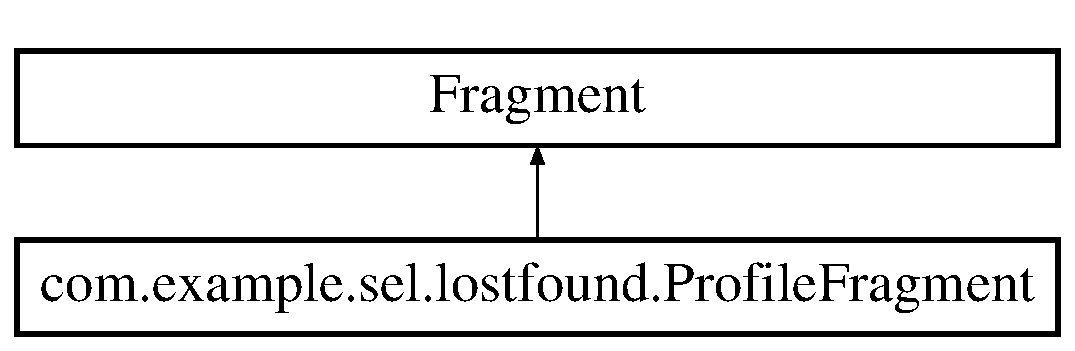
\includegraphics[height=2.000000cm]{classcom_1_1example_1_1sel_1_1lostfound_1_1ProfileFragment}
\end{center}
\end{figure}
\subsection*{Classes}
\begin{DoxyCompactItemize}
\item 
interface \hyperlink{interfacecom_1_1example_1_1sel_1_1lostfound_1_1ProfileFragment_1_1OnFragmentInteractionListener}{On\+Fragment\+Interaction\+Listener}
\end{DoxyCompactItemize}
\subsection*{Public Member Functions}
\begin{DoxyCompactItemize}
\item 
\hyperlink{classcom_1_1example_1_1sel_1_1lostfound_1_1ProfileFragment_aff25ba9b20da50fa32a808f25c0229d6}{Profile\+Fragment} ()
\begin{DoxyCompactList}\small\item\em Required empty public constructor. \end{DoxyCompactList}\item 
void \hyperlink{classcom_1_1example_1_1sel_1_1lostfound_1_1ProfileFragment_a52a51c0a57347d86da5de367f715076f}{on\+Create} (Bundle saved\+Instance\+State)
\item 
void \hyperlink{classcom_1_1example_1_1sel_1_1lostfound_1_1ProfileFragment_a1930f4c070b5d7a4204422f4e0ddc35f}{on\+Activity\+Created} (Bundle saved\+Instance\+State)
\item 
View \hyperlink{classcom_1_1example_1_1sel_1_1lostfound_1_1ProfileFragment_a7bb29240ea89cc1f9c5539dd9117765e}{on\+Create\+View} (Layout\+Inflater inflater, View\+Group container, Bundle saved\+Instance\+State)
\item 
void \hyperlink{classcom_1_1example_1_1sel_1_1lostfound_1_1ProfileFragment_a5d06af34470ca3d940361d9315cd98fb}{on\+Button\+Pressed} (Uri uri)
\item 
void \hyperlink{classcom_1_1example_1_1sel_1_1lostfound_1_1ProfileFragment_a22ef41a710d02636086eb5b6b01a2e1e}{on\+Attach} (Context context)
\item 
void \hyperlink{classcom_1_1example_1_1sel_1_1lostfound_1_1ProfileFragment_a922ba5757676d5642082baaed332dfb1}{on\+Detach} ()
\end{DoxyCompactItemize}
\subsection*{Static Public Member Functions}
\begin{DoxyCompactItemize}
\item 
static \hyperlink{classcom_1_1example_1_1sel_1_1lostfound_1_1ProfileFragment}{Profile\+Fragment} \hyperlink{classcom_1_1example_1_1sel_1_1lostfound_1_1ProfileFragment_a2a0246ef59fbd7dd833eb7db772302c6}{new\+Instance} (String param1, String param2)
\end{DoxyCompactItemize}


\subsection{Detailed Description}
Displays Profile Page, profile information(name, email, profile picture) and posts managed by user. 

\subsection{Constructor \& Destructor Documentation}
\index{com\+::example\+::sel\+::lostfound\+::\+Profile\+Fragment@{com\+::example\+::sel\+::lostfound\+::\+Profile\+Fragment}!Profile\+Fragment@{Profile\+Fragment}}
\index{Profile\+Fragment@{Profile\+Fragment}!com\+::example\+::sel\+::lostfound\+::\+Profile\+Fragment@{com\+::example\+::sel\+::lostfound\+::\+Profile\+Fragment}}
\subsubsection[{\texorpdfstring{Profile\+Fragment()}{ProfileFragment()}}]{\setlength{\rightskip}{0pt plus 5cm}com.\+example.\+sel.\+lostfound.\+Profile\+Fragment.\+Profile\+Fragment (
\begin{DoxyParamCaption}
{}
\end{DoxyParamCaption}
)\hspace{0.3cm}{\ttfamily [inline]}}\hypertarget{classcom_1_1example_1_1sel_1_1lostfound_1_1ProfileFragment_aff25ba9b20da50fa32a808f25c0229d6}{}\label{classcom_1_1example_1_1sel_1_1lostfound_1_1ProfileFragment_aff25ba9b20da50fa32a808f25c0229d6}


Required empty public constructor. 



\subsection{Member Function Documentation}
\index{com\+::example\+::sel\+::lostfound\+::\+Profile\+Fragment@{com\+::example\+::sel\+::lostfound\+::\+Profile\+Fragment}!new\+Instance@{new\+Instance}}
\index{new\+Instance@{new\+Instance}!com\+::example\+::sel\+::lostfound\+::\+Profile\+Fragment@{com\+::example\+::sel\+::lostfound\+::\+Profile\+Fragment}}
\subsubsection[{\texorpdfstring{new\+Instance(\+String param1, String param2)}{newInstance(String param1, String param2)}}]{\setlength{\rightskip}{0pt plus 5cm}static {\bf Profile\+Fragment} com.\+example.\+sel.\+lostfound.\+Profile\+Fragment.\+new\+Instance (
\begin{DoxyParamCaption}
\item[{String}]{param1, }
\item[{String}]{param2}
\end{DoxyParamCaption}
)\hspace{0.3cm}{\ttfamily [inline]}, {\ttfamily [static]}}\hypertarget{classcom_1_1example_1_1sel_1_1lostfound_1_1ProfileFragment_a2a0246ef59fbd7dd833eb7db772302c6}{}\label{classcom_1_1example_1_1sel_1_1lostfound_1_1ProfileFragment_a2a0246ef59fbd7dd833eb7db772302c6}
Use this factory method to create a new instance of this fragment using the provided parameters.


\begin{DoxyParams}{Parameters}
{\em param1} & Parameter 1. \\
\hline
{\em param2} & Parameter 2. \\
\hline
\end{DoxyParams}
\begin{DoxyReturn}{Returns}
A new instance of fragment \hyperlink{classcom_1_1example_1_1sel_1_1lostfound_1_1ProfileFragment}{Profile\+Fragment}. \textbackslash{} 
\end{DoxyReturn}
\index{com\+::example\+::sel\+::lostfound\+::\+Profile\+Fragment@{com\+::example\+::sel\+::lostfound\+::\+Profile\+Fragment}!on\+Activity\+Created@{on\+Activity\+Created}}
\index{on\+Activity\+Created@{on\+Activity\+Created}!com\+::example\+::sel\+::lostfound\+::\+Profile\+Fragment@{com\+::example\+::sel\+::lostfound\+::\+Profile\+Fragment}}
\subsubsection[{\texorpdfstring{on\+Activity\+Created(\+Bundle saved\+Instance\+State)}{onActivityCreated(Bundle savedInstanceState)}}]{\setlength{\rightskip}{0pt plus 5cm}void com.\+example.\+sel.\+lostfound.\+Profile\+Fragment.\+on\+Activity\+Created (
\begin{DoxyParamCaption}
\item[{Bundle}]{saved\+Instance\+State}
\end{DoxyParamCaption}
)\hspace{0.3cm}{\ttfamily [inline]}}\hypertarget{classcom_1_1example_1_1sel_1_1lostfound_1_1ProfileFragment_a1930f4c070b5d7a4204422f4e0ddc35f}{}\label{classcom_1_1example_1_1sel_1_1lostfound_1_1ProfileFragment_a1930f4c070b5d7a4204422f4e0ddc35f}
\textbackslash{} \index{com\+::example\+::sel\+::lostfound\+::\+Profile\+Fragment@{com\+::example\+::sel\+::lostfound\+::\+Profile\+Fragment}!on\+Attach@{on\+Attach}}
\index{on\+Attach@{on\+Attach}!com\+::example\+::sel\+::lostfound\+::\+Profile\+Fragment@{com\+::example\+::sel\+::lostfound\+::\+Profile\+Fragment}}
\subsubsection[{\texorpdfstring{on\+Attach(\+Context context)}{onAttach(Context context)}}]{\setlength{\rightskip}{0pt plus 5cm}void com.\+example.\+sel.\+lostfound.\+Profile\+Fragment.\+on\+Attach (
\begin{DoxyParamCaption}
\item[{Context}]{context}
\end{DoxyParamCaption}
)\hspace{0.3cm}{\ttfamily [inline]}}\hypertarget{classcom_1_1example_1_1sel_1_1lostfound_1_1ProfileFragment_a22ef41a710d02636086eb5b6b01a2e1e}{}\label{classcom_1_1example_1_1sel_1_1lostfound_1_1ProfileFragment_a22ef41a710d02636086eb5b6b01a2e1e}
\textbackslash{} \index{com\+::example\+::sel\+::lostfound\+::\+Profile\+Fragment@{com\+::example\+::sel\+::lostfound\+::\+Profile\+Fragment}!on\+Button\+Pressed@{on\+Button\+Pressed}}
\index{on\+Button\+Pressed@{on\+Button\+Pressed}!com\+::example\+::sel\+::lostfound\+::\+Profile\+Fragment@{com\+::example\+::sel\+::lostfound\+::\+Profile\+Fragment}}
\subsubsection[{\texorpdfstring{on\+Button\+Pressed(\+Uri uri)}{onButtonPressed(Uri uri)}}]{\setlength{\rightskip}{0pt plus 5cm}void com.\+example.\+sel.\+lostfound.\+Profile\+Fragment.\+on\+Button\+Pressed (
\begin{DoxyParamCaption}
\item[{Uri}]{uri}
\end{DoxyParamCaption}
)\hspace{0.3cm}{\ttfamily [inline]}}\hypertarget{classcom_1_1example_1_1sel_1_1lostfound_1_1ProfileFragment_a5d06af34470ca3d940361d9315cd98fb}{}\label{classcom_1_1example_1_1sel_1_1lostfound_1_1ProfileFragment_a5d06af34470ca3d940361d9315cd98fb}
\textbackslash{} \index{com\+::example\+::sel\+::lostfound\+::\+Profile\+Fragment@{com\+::example\+::sel\+::lostfound\+::\+Profile\+Fragment}!on\+Create@{on\+Create}}
\index{on\+Create@{on\+Create}!com\+::example\+::sel\+::lostfound\+::\+Profile\+Fragment@{com\+::example\+::sel\+::lostfound\+::\+Profile\+Fragment}}
\subsubsection[{\texorpdfstring{on\+Create(\+Bundle saved\+Instance\+State)}{onCreate(Bundle savedInstanceState)}}]{\setlength{\rightskip}{0pt plus 5cm}void com.\+example.\+sel.\+lostfound.\+Profile\+Fragment.\+on\+Create (
\begin{DoxyParamCaption}
\item[{Bundle}]{saved\+Instance\+State}
\end{DoxyParamCaption}
)\hspace{0.3cm}{\ttfamily [inline]}}\hypertarget{classcom_1_1example_1_1sel_1_1lostfound_1_1ProfileFragment_a52a51c0a57347d86da5de367f715076f}{}\label{classcom_1_1example_1_1sel_1_1lostfound_1_1ProfileFragment_a52a51c0a57347d86da5de367f715076f}
\textbackslash{} \index{com\+::example\+::sel\+::lostfound\+::\+Profile\+Fragment@{com\+::example\+::sel\+::lostfound\+::\+Profile\+Fragment}!on\+Create\+View@{on\+Create\+View}}
\index{on\+Create\+View@{on\+Create\+View}!com\+::example\+::sel\+::lostfound\+::\+Profile\+Fragment@{com\+::example\+::sel\+::lostfound\+::\+Profile\+Fragment}}
\subsubsection[{\texorpdfstring{on\+Create\+View(\+Layout\+Inflater inflater, View\+Group container, Bundle saved\+Instance\+State)}{onCreateView(LayoutInflater inflater, ViewGroup container, Bundle savedInstanceState)}}]{\setlength{\rightskip}{0pt plus 5cm}View com.\+example.\+sel.\+lostfound.\+Profile\+Fragment.\+on\+Create\+View (
\begin{DoxyParamCaption}
\item[{Layout\+Inflater}]{inflater, }
\item[{View\+Group}]{container, }
\item[{Bundle}]{saved\+Instance\+State}
\end{DoxyParamCaption}
)\hspace{0.3cm}{\ttfamily [inline]}}\hypertarget{classcom_1_1example_1_1sel_1_1lostfound_1_1ProfileFragment_a7bb29240ea89cc1f9c5539dd9117765e}{}\label{classcom_1_1example_1_1sel_1_1lostfound_1_1ProfileFragment_a7bb29240ea89cc1f9c5539dd9117765e}
\textbackslash{} \index{com\+::example\+::sel\+::lostfound\+::\+Profile\+Fragment@{com\+::example\+::sel\+::lostfound\+::\+Profile\+Fragment}!on\+Detach@{on\+Detach}}
\index{on\+Detach@{on\+Detach}!com\+::example\+::sel\+::lostfound\+::\+Profile\+Fragment@{com\+::example\+::sel\+::lostfound\+::\+Profile\+Fragment}}
\subsubsection[{\texorpdfstring{on\+Detach()}{onDetach()}}]{\setlength{\rightskip}{0pt plus 5cm}void com.\+example.\+sel.\+lostfound.\+Profile\+Fragment.\+on\+Detach (
\begin{DoxyParamCaption}
{}
\end{DoxyParamCaption}
)\hspace{0.3cm}{\ttfamily [inline]}}\hypertarget{classcom_1_1example_1_1sel_1_1lostfound_1_1ProfileFragment_a922ba5757676d5642082baaed332dfb1}{}\label{classcom_1_1example_1_1sel_1_1lostfound_1_1ProfileFragment_a922ba5757676d5642082baaed332dfb1}
\textbackslash{} 

The documentation for this class was generated from the following file\+:\begin{DoxyCompactItemize}
\item 
Profile\+Fragment.\+java\end{DoxyCompactItemize}

\hypertarget{interfacecom_1_1example_1_1sel_1_1lostfound_1_1ScriptRunner_1_1ScriptFinishListener}{}\section{com.\+example.\+sel.\+lostfound.\+Script\+Runner.\+Script\+Finish\+Listener Interface Reference}
\label{interfacecom_1_1example_1_1sel_1_1lostfound_1_1ScriptRunner_1_1ScriptFinishListener}\index{com.\+example.\+sel.\+lostfound.\+Script\+Runner.\+Script\+Finish\+Listener@{com.\+example.\+sel.\+lostfound.\+Script\+Runner.\+Script\+Finish\+Listener}}
\subsection*{Public Member Functions}
\begin{DoxyCompactItemize}
\item 
void {\bfseries finish} (String result, int result\+Code)\hypertarget{interfacecom_1_1example_1_1sel_1_1lostfound_1_1ScriptRunner_1_1ScriptFinishListener_a4e61bdd721e7e7e49d26ffef8d559426}{}\label{interfacecom_1_1example_1_1sel_1_1lostfound_1_1ScriptRunner_1_1ScriptFinishListener_a4e61bdd721e7e7e49d26ffef8d559426}

\end{DoxyCompactItemize}


The documentation for this interface was generated from the following file\+:\begin{DoxyCompactItemize}
\item 
Script\+Runner.\+java\end{DoxyCompactItemize}

\hypertarget{classcom_1_1example_1_1sel_1_1lostfound_1_1ScriptRunner}{\section{com.\-example.\-sel.\-lostfound.\-Script\-Runner \-Class \-Reference}
\label{classcom_1_1example_1_1sel_1_1lostfound_1_1ScriptRunner}\index{com.\-example.\-sel.\-lostfound.\-Script\-Runner@{com.\-example.\-sel.\-lostfound.\-Script\-Runner}}
}


\-Inherits \-Async\-Task$<$ String, Void, String $>$.

\subsection*{\-Classes}
\begin{DoxyCompactItemize}
\item 
interface \hyperlink{interfacecom_1_1example_1_1sel_1_1lostfound_1_1ScriptRunner_1_1ScriptFinishListener}{\-Script\-Finish\-Listener}
\end{DoxyCompactItemize}
\subsection*{\-Public \-Member \-Functions}
\begin{DoxyCompactItemize}
\item 
\hypertarget{classcom_1_1example_1_1sel_1_1lostfound_1_1ScriptRunner_a89fe364ebf708a526d2271b2aaad65dc}{{\bfseries \-Script\-Runner} (\hyperlink{interfacecom_1_1example_1_1sel_1_1lostfound_1_1ScriptRunner_1_1ScriptFinishListener}{\-Script\-Finish\-Listener} listener)}\label{classcom_1_1example_1_1sel_1_1lostfound_1_1ScriptRunner_a89fe364ebf708a526d2271b2aaad65dc}

\item 
\hypertarget{classcom_1_1example_1_1sel_1_1lostfound_1_1ScriptRunner_a9f6500f6f9fda5c4230dbbba9724b8bd}{boolean {\bfseries get\-Is\-Done} ()}\label{classcom_1_1example_1_1sel_1_1lostfound_1_1ScriptRunner_a9f6500f6f9fda5c4230dbbba9724b8bd}

\end{DoxyCompactItemize}
\subsection*{\-Static \-Public \-Attributes}
\begin{DoxyCompactItemize}
\item 
\hypertarget{classcom_1_1example_1_1sel_1_1lostfound_1_1ScriptRunner_af663271a5e699ad47264102b5445799e}{static final int {\bfseries \-S\-U\-C\-C\-E\-S\-S} = 0}\label{classcom_1_1example_1_1sel_1_1lostfound_1_1ScriptRunner_af663271a5e699ad47264102b5445799e}

\item 
\hypertarget{classcom_1_1example_1_1sel_1_1lostfound_1_1ScriptRunner_af872e324d4d349db617f9511009901a9}{static final int {\bfseries \-F\-A\-I\-L} = 1}\label{classcom_1_1example_1_1sel_1_1lostfound_1_1ScriptRunner_af872e324d4d349db617f9511009901a9}

\item 
\hypertarget{classcom_1_1example_1_1sel_1_1lostfound_1_1ScriptRunner_a6b8f5d1e77298c2f260fd7ef9502650d}{static final \-String {\bfseries \-E\-N\-D\-P\-O\-I\-N\-T} = \char`\"{}http\-://52.\-38.\-30.\-3/\char`\"{}}\label{classcom_1_1example_1_1sel_1_1lostfound_1_1ScriptRunner_a6b8f5d1e77298c2f260fd7ef9502650d}

\end{DoxyCompactItemize}
\subsection*{\-Protected \-Member \-Functions}
\begin{DoxyCompactItemize}
\item 
\hypertarget{classcom_1_1example_1_1sel_1_1lostfound_1_1ScriptRunner_a9050c944957b5b8fcacc9d2cba6f3b71}{\-String {\bfseries do\-In\-Background} (\-String...\-s)}\label{classcom_1_1example_1_1sel_1_1lostfound_1_1ScriptRunner_a9050c944957b5b8fcacc9d2cba6f3b71}

\item 
\hypertarget{classcom_1_1example_1_1sel_1_1lostfound_1_1ScriptRunner_affce5629df2ecd60a45f3c707b996955}{void {\bfseries on\-Post\-Execute} (\-String result)}\label{classcom_1_1example_1_1sel_1_1lostfound_1_1ScriptRunner_affce5629df2ecd60a45f3c707b996955}

\end{DoxyCompactItemize}


\-The documentation for this class was generated from the following file\-:\begin{DoxyCompactItemize}
\item 
\-Script\-Runner.\-java\end{DoxyCompactItemize}

\hypertarget{classcom_1_1example_1_1sel_1_1lostfound_1_1SpinnerAdapter}{}\section{com.\+example.\+sel.\+lostfound.\+Spinner\+Adapter Class Reference}
\label{classcom_1_1example_1_1sel_1_1lostfound_1_1SpinnerAdapter}\index{com.\+example.\+sel.\+lostfound.\+Spinner\+Adapter@{com.\+example.\+sel.\+lostfound.\+Spinner\+Adapter}}
Inheritance diagram for com.\+example.\+sel.\+lostfound.\+Spinner\+Adapter\+:\begin{figure}[H]
\begin{center}
\leavevmode
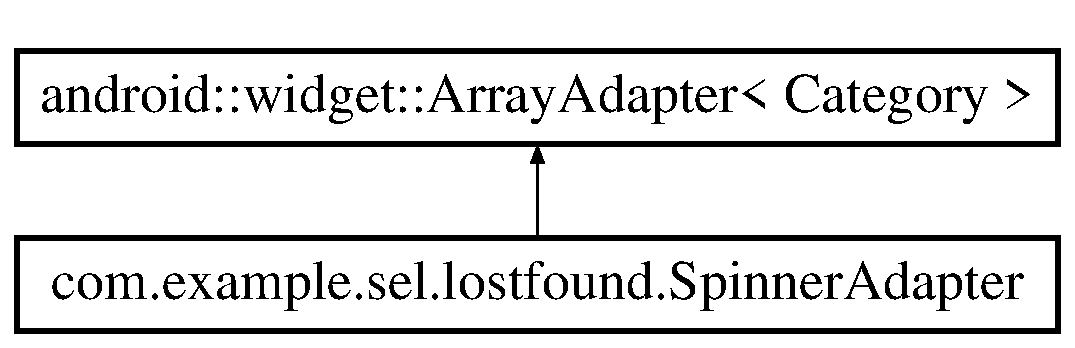
\includegraphics[height=2.000000cm]{classcom_1_1example_1_1sel_1_1lostfound_1_1SpinnerAdapter}
\end{center}
\end{figure}
\subsection*{Public Member Functions}
\begin{DoxyCompactItemize}
\item 
int {\bfseries get\+Count} ()\hypertarget{classcom_1_1example_1_1sel_1_1lostfound_1_1SpinnerAdapter_a9ee3f8a3ee4642cc4379a4fc710a4484}{}\label{classcom_1_1example_1_1sel_1_1lostfound_1_1SpinnerAdapter_a9ee3f8a3ee4642cc4379a4fc710a4484}

\item 
\hyperlink{classcom_1_1example_1_1sel_1_1lostfound_1_1Category}{Category} {\bfseries get\+Item} (int position)\hypertarget{classcom_1_1example_1_1sel_1_1lostfound_1_1SpinnerAdapter_a48949a737b70991a11fe5f45e6c0b6c1}{}\label{classcom_1_1example_1_1sel_1_1lostfound_1_1SpinnerAdapter_a48949a737b70991a11fe5f45e6c0b6c1}

\item 
long {\bfseries get\+Item\+Id} (int position)\hypertarget{classcom_1_1example_1_1sel_1_1lostfound_1_1SpinnerAdapter_a248484bdf819294d3bdc8f6db635c673}{}\label{classcom_1_1example_1_1sel_1_1lostfound_1_1SpinnerAdapter_a248484bdf819294d3bdc8f6db635c673}

\item 
{\bfseries Spinner\+Adapter} (Context context, int resource, List$<$ \hyperlink{classcom_1_1example_1_1sel_1_1lostfound_1_1Category}{Category} $>$ objects)\hypertarget{classcom_1_1example_1_1sel_1_1lostfound_1_1SpinnerAdapter_a9cbc724bbe142a941090cc9bf5b8bcb6}{}\label{classcom_1_1example_1_1sel_1_1lostfound_1_1SpinnerAdapter_a9cbc724bbe142a941090cc9bf5b8bcb6}

\item 
View {\bfseries get\+View} (int position, View convert\+View, View\+Group parent)\hypertarget{classcom_1_1example_1_1sel_1_1lostfound_1_1SpinnerAdapter_ac19132459aeaef196c367a156bb03e0e}{}\label{classcom_1_1example_1_1sel_1_1lostfound_1_1SpinnerAdapter_ac19132459aeaef196c367a156bb03e0e}

\item 
View {\bfseries get\+Drop\+Down\+View} (int position, View convert\+View, View\+Group parent)\hypertarget{classcom_1_1example_1_1sel_1_1lostfound_1_1SpinnerAdapter_a338cec7659aa976e986e4d1c843d4041}{}\label{classcom_1_1example_1_1sel_1_1lostfound_1_1SpinnerAdapter_a338cec7659aa976e986e4d1c843d4041}

\end{DoxyCompactItemize}


\subsection{Detailed Description}
Created by achu on 12-\/04-\/2016. 

The documentation for this class was generated from the following file\+:\begin{DoxyCompactItemize}
\item 
Spinner\+Adapter.\+java\end{DoxyCompactItemize}

\hypertarget{classcom_1_1example_1_1sel_1_1lostfound_1_1SubscribeAdapter}{}\section{com.\+example.\+sel.\+lostfound.\+Subscribe\+Adapter Class Reference}
\label{classcom_1_1example_1_1sel_1_1lostfound_1_1SubscribeAdapter}\index{com.\+example.\+sel.\+lostfound.\+Subscribe\+Adapter@{com.\+example.\+sel.\+lostfound.\+Subscribe\+Adapter}}
Inheritance diagram for com.\+example.\+sel.\+lostfound.\+Subscribe\+Adapter\+:\begin{figure}[H]
\begin{center}
\leavevmode
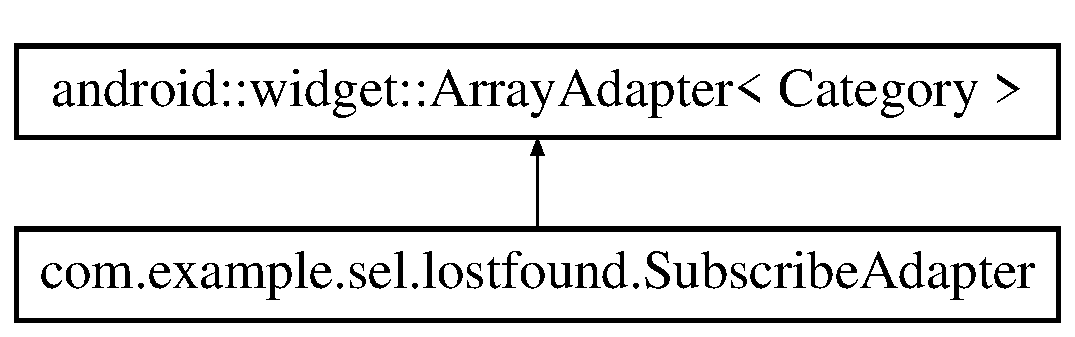
\includegraphics[height=2.000000cm]{classcom_1_1example_1_1sel_1_1lostfound_1_1SubscribeAdapter}
\end{center}
\end{figure}
\subsection*{Classes}
\begin{DoxyCompactItemize}
\item 
class {\bfseries Subscribe\+Holder}
\end{DoxyCompactItemize}
\subsection*{Public Member Functions}
\begin{DoxyCompactItemize}
\item 
{\bfseries Subscribe\+Adapter} (Context context, int resource, List$<$ \hyperlink{classcom_1_1example_1_1sel_1_1lostfound_1_1Category}{Category} $>$ objects)\hypertarget{classcom_1_1example_1_1sel_1_1lostfound_1_1SubscribeAdapter_ad5670875fa5fcc236d9c794303f04369}{}\label{classcom_1_1example_1_1sel_1_1lostfound_1_1SubscribeAdapter_ad5670875fa5fcc236d9c794303f04369}

\item 
View {\bfseries get\+View} (int position, View convert\+View, View\+Group parent)\hypertarget{classcom_1_1example_1_1sel_1_1lostfound_1_1SubscribeAdapter_a942f195e46312808aff706a8a4e15e02}{}\label{classcom_1_1example_1_1sel_1_1lostfound_1_1SubscribeAdapter_a942f195e46312808aff706a8a4e15e02}

\end{DoxyCompactItemize}


\subsection{Detailed Description}
Created by achu on 14-\/04-\/2016. 

The documentation for this class was generated from the following file\+:\begin{DoxyCompactItemize}
\item 
Subscribe\+Adapter.\+java\end{DoxyCompactItemize}

<<<<<<< HEAD
\hypertarget{classcom_1_1example_1_1sel_1_1lostfound_1_1SubscribeFragment}{\section{com.\-example.\-sel.\-lostfound.\-Subscribe\-Fragment Class Reference}
\label{classcom_1_1example_1_1sel_1_1lostfound_1_1SubscribeFragment}\index{com.\-example.\-sel.\-lostfound.\-Subscribe\-Fragment@{com.\-example.\-sel.\-lostfound.\-Subscribe\-Fragment}}
}
Inheritance diagram for com.\-example.\-sel.\-lostfound.\-Subscribe\-Fragment\-:\begin{figure}[H]
\begin{center}
\leavevmode
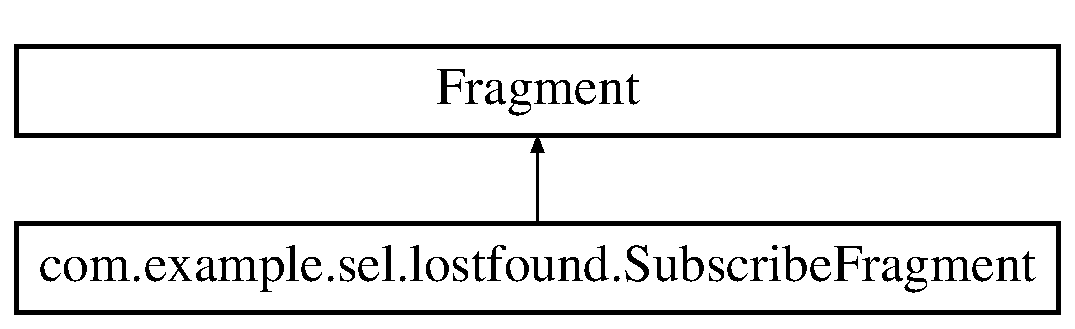
\includegraphics[height=2.000000cm]{classcom_1_1example_1_1sel_1_1lostfound_1_1SubscribeFragment}
\end{center}
\end{figure}
\subsection*{Classes}
\begin{DoxyCompactItemize}
\item 
interface \hyperlink{interfacecom_1_1example_1_1sel_1_1lostfound_1_1SubscribeFragment_1_1OnFragmentInteractionListener}{On\-Fragment\-Interaction\-Listener}
\end{DoxyCompactItemize}
\subsection*{Public Member Functions}
\begin{DoxyCompactItemize}
\item 
\hypertarget{classcom_1_1example_1_1sel_1_1lostfound_1_1SubscribeFragment_a7f0cd7584a12208f6cc9e3c8fb1fd680}{void {\bfseries on\-Create} (Bundle saved\-Instance\-State)}\label{classcom_1_1example_1_1sel_1_1lostfound_1_1SubscribeFragment_a7f0cd7584a12208f6cc9e3c8fb1fd680}

\item 
\hypertarget{classcom_1_1example_1_1sel_1_1lostfound_1_1SubscribeFragment_a6daae3059443ffda76c69cc51f2d9dec}{void {\bfseries on\-Activity\-Created} (Bundle saved\-Instance\-State)}\label{classcom_1_1example_1_1sel_1_1lostfound_1_1SubscribeFragment_a6daae3059443ffda76c69cc51f2d9dec}

\item 
\hypertarget{classcom_1_1example_1_1sel_1_1lostfound_1_1SubscribeFragment_a521224b1fa6e19b441cd064c636137f1}{View {\bfseries on\-Create\-View} (Layout\-Inflater inflater, View\-Group container, Bundle saved\-Instance\-State)}\label{classcom_1_1example_1_1sel_1_1lostfound_1_1SubscribeFragment_a521224b1fa6e19b441cd064c636137f1}

\item 
\hypertarget{classcom_1_1example_1_1sel_1_1lostfound_1_1SubscribeFragment_a018589e8d66394f7c11ec44d996fbdcf}{void {\bfseries on\-Button\-Pressed} (Uri uri)}\label{classcom_1_1example_1_1sel_1_1lostfound_1_1SubscribeFragment_a018589e8d66394f7c11ec44d996fbdcf}

\item 
\hypertarget{classcom_1_1example_1_1sel_1_1lostfound_1_1SubscribeFragment_adc31ba19040d95af6b9ab1a11677f93d}{void {\bfseries on\-Attach} (Context context)}\label{classcom_1_1example_1_1sel_1_1lostfound_1_1SubscribeFragment_adc31ba19040d95af6b9ab1a11677f93d}
=======
\hypertarget{classcom_1_1example_1_1sel_1_1lostfound_1_1SubscribeFragment}{\section{com.\-example.\-sel.\-lostfound.\-Subscribe\-Fragment \-Class \-Reference}
\label{classcom_1_1example_1_1sel_1_1lostfound_1_1SubscribeFragment}\index{com.\-example.\-sel.\-lostfound.\-Subscribe\-Fragment@{com.\-example.\-sel.\-lostfound.\-Subscribe\-Fragment}}
}


\-Inherits \-Fragment.

\subsection*{\-Classes}
\begin{DoxyCompactItemize}
\item 
interface \hyperlink{interfacecom_1_1example_1_1sel_1_1lostfound_1_1SubscribeFragment_1_1OnFragmentInteractionListener}{\-On\-Fragment\-Interaction\-Listener}
\end{DoxyCompactItemize}
\subsection*{\-Public \-Member \-Functions}
\begin{DoxyCompactItemize}
\item 
\hypertarget{classcom_1_1example_1_1sel_1_1lostfound_1_1SubscribeFragment_a7f0cd7584a12208f6cc9e3c8fb1fd680}{void {\bfseries on\-Create} (\-Bundle saved\-Instance\-State)}\label{classcom_1_1example_1_1sel_1_1lostfound_1_1SubscribeFragment_a7f0cd7584a12208f6cc9e3c8fb1fd680}

\item 
\hypertarget{classcom_1_1example_1_1sel_1_1lostfound_1_1SubscribeFragment_a6daae3059443ffda76c69cc51f2d9dec}{void {\bfseries on\-Activity\-Created} (\-Bundle saved\-Instance\-State)}\label{classcom_1_1example_1_1sel_1_1lostfound_1_1SubscribeFragment_a6daae3059443ffda76c69cc51f2d9dec}

\item 
\hypertarget{classcom_1_1example_1_1sel_1_1lostfound_1_1SubscribeFragment_a521224b1fa6e19b441cd064c636137f1}{\-View {\bfseries on\-Create\-View} (\-Layout\-Inflater inflater, \-View\-Group container, \-Bundle saved\-Instance\-State)}\label{classcom_1_1example_1_1sel_1_1lostfound_1_1SubscribeFragment_a521224b1fa6e19b441cd064c636137f1}

\item 
\hypertarget{classcom_1_1example_1_1sel_1_1lostfound_1_1SubscribeFragment_a018589e8d66394f7c11ec44d996fbdcf}{void {\bfseries on\-Button\-Pressed} (\-Uri uri)}\label{classcom_1_1example_1_1sel_1_1lostfound_1_1SubscribeFragment_a018589e8d66394f7c11ec44d996fbdcf}

\item 
\hypertarget{classcom_1_1example_1_1sel_1_1lostfound_1_1SubscribeFragment_adc31ba19040d95af6b9ab1a11677f93d}{void {\bfseries on\-Attach} (\-Context context)}\label{classcom_1_1example_1_1sel_1_1lostfound_1_1SubscribeFragment_adc31ba19040d95af6b9ab1a11677f93d}
>>>>>>> 0bbb2bc5f31f033d772ef4573f66c50564006509

\item 
\hypertarget{classcom_1_1example_1_1sel_1_1lostfound_1_1SubscribeFragment_a756f69f0e7f8f456fbbb077502d9494f}{void {\bfseries on\-Detach} ()}\label{classcom_1_1example_1_1sel_1_1lostfound_1_1SubscribeFragment_a756f69f0e7f8f456fbbb077502d9494f}

\end{DoxyCompactItemize}
<<<<<<< HEAD
\subsection*{Static Public Member Functions}
\begin{DoxyCompactItemize}
\item 
static \hyperlink{classcom_1_1example_1_1sel_1_1lostfound_1_1SubscribeFragment}{Subscribe\-Fragment} \hyperlink{classcom_1_1example_1_1sel_1_1lostfound_1_1SubscribeFragment_ac622c73212970653128ddfb06d38572a}{new\-Instance} (String param1, String param2)
\end{DoxyCompactItemize}


\subsection{Detailed Description}
Created by Rohit G on 4/2/2016. A simple \hyperlink{}{Fragment} subclass. Activities that contain this fragment must implement the \hyperlink{interfacecom_1_1example_1_1sel_1_1lostfound_1_1SubscribeFragment_1_1OnFragmentInteractionListener}{Subscribe\-Fragment.\-On\-Fragment\-Interaction\-Listener} interface to handle interaction events. Use the \hyperlink{classcom_1_1example_1_1sel_1_1lostfound_1_1SubscribeFragment_ac622c73212970653128ddfb06d38572a}{Subscribe\-Fragment\#new\-Instance} factory method to create an instance of this fragment. 

\subsection{Member Function Documentation}
\hypertarget{classcom_1_1example_1_1sel_1_1lostfound_1_1SubscribeFragment_ac622c73212970653128ddfb06d38572a}{\index{com\-::example\-::sel\-::lostfound\-::\-Subscribe\-Fragment@{com\-::example\-::sel\-::lostfound\-::\-Subscribe\-Fragment}!new\-Instance@{new\-Instance}}
\index{new\-Instance@{new\-Instance}!com::example::sel::lostfound::SubscribeFragment@{com\-::example\-::sel\-::lostfound\-::\-Subscribe\-Fragment}}
\subsubsection[{new\-Instance}]{\setlength{\rightskip}{0pt plus 5cm}static {\bf Subscribe\-Fragment} com.\-example.\-sel.\-lostfound.\-Subscribe\-Fragment.\-new\-Instance (
\begin{DoxyParamCaption}
\item[{String}]{param1, }
\item[{String}]{param2}
\end{DoxyParamCaption}
)\hspace{0.3cm}{\ttfamily [inline]}, {\ttfamily [static]}}}\label{classcom_1_1example_1_1sel_1_1lostfound_1_1SubscribeFragment_ac622c73212970653128ddfb06d38572a}
Use this factory method to create a new instance of this fragment using the provided parameters.


\begin{DoxyParams}{Parameters}
{\em param1} & Parameter 1. \\
\hline
{\em param2} & Parameter 2. \\
\hline
\end{DoxyParams}
\begin{DoxyReturn}{Returns}
A new instance of fragment \hyperlink{classcom_1_1example_1_1sel_1_1lostfound_1_1SubscribeFragment}{Subscribe\-Fragment}. 
\end{DoxyReturn}


The documentation for this class was generated from the following file\-:\begin{DoxyCompactItemize}
\item 
Subscribe\-Fragment.\-java\end{DoxyCompactItemize}
=======
\subsection*{\-Static \-Public \-Member \-Functions}
\begin{DoxyCompactItemize}
\item 
static \hyperlink{classcom_1_1example_1_1sel_1_1lostfound_1_1SubscribeFragment}{\-Subscribe\-Fragment} \hyperlink{classcom_1_1example_1_1sel_1_1lostfound_1_1SubscribeFragment_ac622c73212970653128ddfb06d38572a}{new\-Instance} (\-String param1, \-String param2)
\end{DoxyCompactItemize}
\subsection*{\-Package \-Attributes}
\begin{DoxyCompactItemize}
\item 
\hypertarget{classcom_1_1example_1_1sel_1_1lostfound_1_1SubscribeFragment_ac660e1e7a61b24c751595962f5c3495d}{\-String {\bfseries post\-Address} = \char`\"{}http\-://52.\-38.\-30.\-3/getallcat.\-php\char`\"{}}\label{classcom_1_1example_1_1sel_1_1lostfound_1_1SubscribeFragment_ac660e1e7a61b24c751595962f5c3495d}

\item 
\hypertarget{classcom_1_1example_1_1sel_1_1lostfound_1_1SubscribeFragment_a9f0d6661e6347af9b678abd1e883a602}{\-String {\bfseries post\-Address2} = \char`\"{}http\-://52.\-38.\-30.\-3/getsubscribedcat.\-php\char`\"{}}\label{classcom_1_1example_1_1sel_1_1lostfound_1_1SubscribeFragment_a9f0d6661e6347af9b678abd1e883a602}

\item 
\hypertarget{classcom_1_1example_1_1sel_1_1lostfound_1_1SubscribeFragment_afcc89336a65d7e088ce327db4927a78f}{\-Button {\bfseries subscribe\-\_\-button}}\label{classcom_1_1example_1_1sel_1_1lostfound_1_1SubscribeFragment_afcc89336a65d7e088ce327db4927a78f}

\end{DoxyCompactItemize}


\subsection{\-Detailed \-Description}
\-A simple \hyperlink{}{\-Fragment} subclass. \-Activities that contain this fragment must implement the \hyperlink{interfacecom_1_1example_1_1sel_1_1lostfound_1_1SubscribeFragment_1_1OnFragmentInteractionListener}{\-Subscribe\-Fragment.\-On\-Fragment\-Interaction\-Listener} interface to handle interaction events. \-Use the \hyperlink{classcom_1_1example_1_1sel_1_1lostfound_1_1SubscribeFragment_ac622c73212970653128ddfb06d38572a}{\-Subscribe\-Fragment\#new\-Instance} factory method to create an instance of this fragment. 

\subsection{\-Member \-Function \-Documentation}
\hypertarget{classcom_1_1example_1_1sel_1_1lostfound_1_1SubscribeFragment_ac622c73212970653128ddfb06d38572a}{\index{com\-::example\-::sel\-::lostfound\-::\-Subscribe\-Fragment@{com\-::example\-::sel\-::lostfound\-::\-Subscribe\-Fragment}!new\-Instance@{new\-Instance}}
\index{new\-Instance@{new\-Instance}!com::example::sel::lostfound::SubscribeFragment@{com\-::example\-::sel\-::lostfound\-::\-Subscribe\-Fragment}}
\subsubsection[{new\-Instance}]{\setlength{\rightskip}{0pt plus 5cm}static {\bf \-Subscribe\-Fragment} {\bf com.\-example.\-sel.\-lostfound.\-Subscribe\-Fragment.\-new\-Instance} (
\begin{DoxyParamCaption}
\item[{\-String}]{param1, }
\item[{\-String}]{param2}
\end{DoxyParamCaption}
)\hspace{0.3cm}{\ttfamily  \mbox{[}inline, static\mbox{]}}}}\label{classcom_1_1example_1_1sel_1_1lostfound_1_1SubscribeFragment_ac622c73212970653128ddfb06d38572a}
\-Use this factory method to create a new instance of this fragment using the provided parameters.


\begin{DoxyParams}{\-Parameters}
{\em param1} & \-Parameter 1. \\
\hline
{\em param2} & \-Parameter 2. \\
\hline
\end{DoxyParams}
\begin{DoxyReturn}{\-Returns}
\-A new instance of fragment \hyperlink{classcom_1_1example_1_1sel_1_1lostfound_1_1SubscribeFragment}{\-Subscribe\-Fragment}. 
\end{DoxyReturn}


\-The documentation for this class was generated from the following file\-:\begin{DoxyCompactItemize}
\item 
\-Subscribe\-Fragment.\-java\end{DoxyCompactItemize}
>>>>>>> 0bbb2bc5f31f033d772ef4573f66c50564006509

\hypertarget{classcom_1_1example_1_1sel_1_1lostfound_1_1UserPost}{\section{com.\-example.\-sel.\-lostfound.\-User\-Post Class Reference}
\label{classcom_1_1example_1_1sel_1_1lostfound_1_1UserPost}\index{com.\-example.\-sel.\-lostfound.\-User\-Post@{com.\-example.\-sel.\-lostfound.\-User\-Post}}
}
\subsection*{Public Member Functions}
\begin{DoxyCompactItemize}
\item 
\hypertarget{classcom_1_1example_1_1sel_1_1lostfound_1_1UserPost_a115af0c6a558f34125aa8bedc5edf6a1}{{\bfseries User\-Post} (String posttype, String title, String description, String categoryid, String postid, String time, String date, String location)}\label{classcom_1_1example_1_1sel_1_1lostfound_1_1UserPost_a115af0c6a558f34125aa8bedc5edf6a1}

\item 
\hypertarget{classcom_1_1example_1_1sel_1_1lostfound_1_1UserPost_abda6328cdfe66f43f6ffdf73b87d91c6}{String {\bfseries get\-Posttype} ()}\label{classcom_1_1example_1_1sel_1_1lostfound_1_1UserPost_abda6328cdfe66f43f6ffdf73b87d91c6}

\item 
\hypertarget{classcom_1_1example_1_1sel_1_1lostfound_1_1UserPost_a2123e2a801f39239ad7713e4df64d603}{void {\bfseries set\-Posttype} (String posttype)}\label{classcom_1_1example_1_1sel_1_1lostfound_1_1UserPost_a2123e2a801f39239ad7713e4df64d603}

\item 
\hypertarget{classcom_1_1example_1_1sel_1_1lostfound_1_1UserPost_a7ca77f66b088c6ffe832467a90e52dfd}{String {\bfseries get\-Title} ()}\label{classcom_1_1example_1_1sel_1_1lostfound_1_1UserPost_a7ca77f66b088c6ffe832467a90e52dfd}

\item 
\hypertarget{classcom_1_1example_1_1sel_1_1lostfound_1_1UserPost_a1ffca3ecc26e1663951a11d830af73f6}{void {\bfseries set\-Title} (String title)}\label{classcom_1_1example_1_1sel_1_1lostfound_1_1UserPost_a1ffca3ecc26e1663951a11d830af73f6}

\item 
\hypertarget{classcom_1_1example_1_1sel_1_1lostfound_1_1UserPost_a356b052bdfc18ab0ece0661ad66a86a0}{String {\bfseries get\-Description} ()}\label{classcom_1_1example_1_1sel_1_1lostfound_1_1UserPost_a356b052bdfc18ab0ece0661ad66a86a0}

\item 
\hypertarget{classcom_1_1example_1_1sel_1_1lostfound_1_1UserPost_a3e6766998b29d8bec4c76213324498fb}{void {\bfseries set\-Description} (String description)}\label{classcom_1_1example_1_1sel_1_1lostfound_1_1UserPost_a3e6766998b29d8bec4c76213324498fb}

\item 
\hypertarget{classcom_1_1example_1_1sel_1_1lostfound_1_1UserPost_ab3772d201f7f05196345d3dc66075189}{String {\bfseries get\-Categoryid} ()}\label{classcom_1_1example_1_1sel_1_1lostfound_1_1UserPost_ab3772d201f7f05196345d3dc66075189}

\item 
\hypertarget{classcom_1_1example_1_1sel_1_1lostfound_1_1UserPost_af7f8a9a859f2c03bb77328b774e4c3bd}{void {\bfseries set\-Categoryid} (String categoryid)}\label{classcom_1_1example_1_1sel_1_1lostfound_1_1UserPost_af7f8a9a859f2c03bb77328b774e4c3bd}

\item 
\hypertarget{classcom_1_1example_1_1sel_1_1lostfound_1_1UserPost_a2f81d7b48aae6ba416e59b6a087e10e7}{String {\bfseries get\-Postid} ()}\label{classcom_1_1example_1_1sel_1_1lostfound_1_1UserPost_a2f81d7b48aae6ba416e59b6a087e10e7}

\item 
\hypertarget{classcom_1_1example_1_1sel_1_1lostfound_1_1UserPost_af10fab9ab95f233876a5961a99292762}{void {\bfseries set\-Postid} (String postid)}\label{classcom_1_1example_1_1sel_1_1lostfound_1_1UserPost_af10fab9ab95f233876a5961a99292762}

\item 
\hypertarget{classcom_1_1example_1_1sel_1_1lostfound_1_1UserPost_a1cfb73a05fe449e7a4772aca1e66ec02}{String {\bfseries get\-Time} ()}\label{classcom_1_1example_1_1sel_1_1lostfound_1_1UserPost_a1cfb73a05fe449e7a4772aca1e66ec02}

\item 
\hypertarget{classcom_1_1example_1_1sel_1_1lostfound_1_1UserPost_a701f3fd781319172374f9d90c4c5c44a}{void {\bfseries set\-Time} (String time)}\label{classcom_1_1example_1_1sel_1_1lostfound_1_1UserPost_a701f3fd781319172374f9d90c4c5c44a}

\item 
\hypertarget{classcom_1_1example_1_1sel_1_1lostfound_1_1UserPost_ae25c6f2fd3481fbdb1ad9cbe43323f24}{String {\bfseries get\-Date} ()}\label{classcom_1_1example_1_1sel_1_1lostfound_1_1UserPost_ae25c6f2fd3481fbdb1ad9cbe43323f24}

\item 
\hypertarget{classcom_1_1example_1_1sel_1_1lostfound_1_1UserPost_a60b0d94eb3abc65675a53f54215af7de}{void {\bfseries set\-Date} (String date)}\label{classcom_1_1example_1_1sel_1_1lostfound_1_1UserPost_a60b0d94eb3abc65675a53f54215af7de}

\item 
\hypertarget{classcom_1_1example_1_1sel_1_1lostfound_1_1UserPost_a270d7e2d632aeaaf74c0157f8cd59dce}{String {\bfseries get\-Location} ()}\label{classcom_1_1example_1_1sel_1_1lostfound_1_1UserPost_a270d7e2d632aeaaf74c0157f8cd59dce}

\item 
\hypertarget{classcom_1_1example_1_1sel_1_1lostfound_1_1UserPost_ad5125a5c2edf33651ace995ae065ecdf}{void {\bfseries set\-Location} (String location)}\label{classcom_1_1example_1_1sel_1_1lostfound_1_1UserPost_ad5125a5c2edf33651ace995ae065ecdf}

\end{DoxyCompactItemize}


\subsection{Detailed Description}
Created by bablu on 4/14/2016. 

The documentation for this class was generated from the following file\-:\begin{DoxyCompactItemize}
\item 
User\-Post.\-java\end{DoxyCompactItemize}

\hypertarget{classcom_1_1example_1_1sel_1_1lostfound_1_1UserPostAdapter}{}\section{com.\+example.\+sel.\+lostfound.\+User\+Post\+Adapter Class Reference}
\label{classcom_1_1example_1_1sel_1_1lostfound_1_1UserPostAdapter}\index{com.\+example.\+sel.\+lostfound.\+User\+Post\+Adapter@{com.\+example.\+sel.\+lostfound.\+User\+Post\+Adapter}}
Inheritance diagram for com.\+example.\+sel.\+lostfound.\+User\+Post\+Adapter\+:\begin{figure}[H]
\begin{center}
\leavevmode
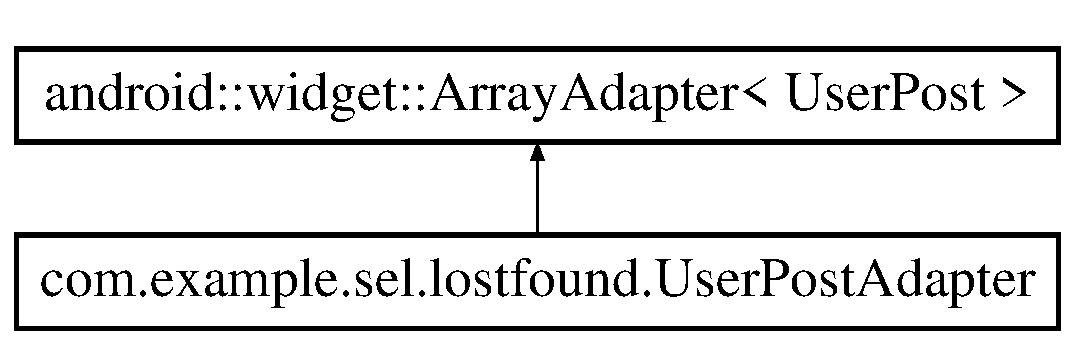
\includegraphics[height=2.000000cm]{classcom_1_1example_1_1sel_1_1lostfound_1_1UserPostAdapter}
\end{center}
\end{figure}
\subsection*{Classes}
\begin{DoxyCompactItemize}
\item 
class {\bfseries User\+Post\+Holder}
\end{DoxyCompactItemize}
\subsection*{Public Member Functions}
\begin{DoxyCompactItemize}
\item 
{\bfseries User\+Post\+Adapter} (Context context, int resource, List$<$ \hyperlink{classcom_1_1example_1_1sel_1_1lostfound_1_1UserPost}{User\+Post} $>$ objects)\hypertarget{classcom_1_1example_1_1sel_1_1lostfound_1_1UserPostAdapter_a8770784429d0552a7472193206396700}{}\label{classcom_1_1example_1_1sel_1_1lostfound_1_1UserPostAdapter_a8770784429d0552a7472193206396700}

\item 
View {\bfseries get\+View} (int position, View convert\+View, View\+Group parent)\hypertarget{classcom_1_1example_1_1sel_1_1lostfound_1_1UserPostAdapter_ab3b3a8f8ee3bb0bf9a8a863209009395}{}\label{classcom_1_1example_1_1sel_1_1lostfound_1_1UserPostAdapter_ab3b3a8f8ee3bb0bf9a8a863209009395}

\end{DoxyCompactItemize}


\subsection{Detailed Description}
Created by bablu on 4/14/2016. 

The documentation for this class was generated from the following file\+:\begin{DoxyCompactItemize}
\item 
User\+Post\+Adapter.\+java\end{DoxyCompactItemize}

%--- End generated contents ---

% Index
\newpage
\phantomsection
\addcontentsline{toc}{chapter}{Index}
\printindex

\end{document}
